\documentclass[12pt]{extarticle} 
%\usepackage{unicode-math}
\usepackage{amsmath,amsfonts,amssymb,amsthm,graphicx,xcolor,natbib,booktabs,tabularx}
%\usepackage[paperwidth=126mm,paperheight=96mm,top=5mm,bottom=5mm,right=5mm,left=5mm]{geometry}
\usepackage[margin=1cm,footskip=5mm]{geometry}
\pagenumbering{gobble}

\usepackage[inline]{enumitem}
\usepackage[BoldFont,SlantFont]{xeCJK}  
\xeCJKsetemboldenfactor{2}
\setCJKmainfont{cwTeX Q Yuan Medium}
%\setCJKmainfont{cwTeX Q Kai Medium}
%\setCJKmainfont{cwTeX Q Ming Medium}
%\setCJKmainfont[AutoFakeSlant=.1,AutoFakeBold=1]{cwTeX Q Kai Medium} 
%\setCJKfamilyfont{kaiv}[Vertical=RotatedGlyphs]{cwTeX Q Medium}
%\setmainfont{texgyrepagella-regular.otf}
%\setmathfont{texgyrepagella-math.otf}
\newcommand{\ds}{\displaystyle}
\newcommand{\ie}{\;\Longrightarrow\;}
\newcommand{\ifff}{\;\Longleftrightarrow\;}
\newcommand{\mi}{\mathrm{i}}
\DeclareMathOperator*{\dom}{dom}
\DeclareMathOperator*{\codom}{codom}
\DeclareMathOperator*{\ran}{ran}
\DeclareMathOperator*{\sgn}{sgn}
\DeclareMathOperator*{\degr}{deg}
\newcommand{\floor}[1]{\lfloor #1 \rfloor}
\newcommand{\ceil}[1]{\lceil #1 \rceil}

\newcommand{\bdiff}[2]{ \frac{\mathrm{d}}{\mathrm{d}#2} \left( #1 \right)}
\newcommand{\ddiff}[3]{ \frac{\mathrm{d}^#1#2}{\mathrm{d}{#3}^#1}}
\newcommand{\half}{\tfrac{1}{2}}
\newcommand{\diff}[2]{ \frac{\mathrm{d}\hfil#1\hfil}{\mathrm{d}#2}}
\newcommand{\difftwo}[2]{ \frac{\mathrm{d^2}\hfil#1\hfil}{\mathrm{d}{#2}^2}}

% figure --> 圖
\renewcommand{\appendixname}{附錄}
\renewcommand{\figurename}{圖}
\renewcommand{\tablename}{表}
\renewcommand{\refname}{參考文獻}

\usepackage{hyperref}
\hypersetup{
    colorlinks,
    linkcolor={red!50!black},
    citecolor={blue!60!black},
    urlcolor={blue!60!black}
    %urlcolor={blue!80!black}
}

\theoremstyle{definition}
\newtheorem*{dfn}{定義}
\newtheorem*{prp}{性質}
\newtheorem*{fact}{結論}
\newtheorem*{thm}{定理}
\newtheorem*{ex}{例}
\newtheorem*{sol}{解}
\newtheorem*{prf}{證}
\newtheorem*{rmk}{註}
\newtheorem*{exe}{習題}

%\setenumerate{label=(\roman*),itemsep=1pt,topsep=3pt}
\newcommand{\myline}{\noindent\makebox[\linewidth]{\rule{\paperwidth}{0.4pt}}}
%\newcommand{\myline}{\textcolor[RGB]{220,220,220}{\rule{\linewidth}{1pt}}}

\usepackage{pgfplots}
\usetikzlibrary{arrows.meta,angles,quotes,patterns}
% axis style, ticks, etc
\pgfplotsset{every axis/.append style={
                   label style={font=\fontsize{4}{4}\selectfont},
                   tick label style={font=\fontsize{4}{4}\selectfont}  
               },
            }
\renewcommand\tabularxcolumn[1]{m{#1}}

%%%%%%%%%%%%%%%%%%%%%%%%%%%%%%%%%%%%%%%%%%%%%%%%%%%%%%%%%%%%%%%%%%%%%

\usepackage{multicol}
\usepackage{ifthen}
\tikzstyle{vertex}=[shape=circle, minimum size=2mm, inner sep=0, fill]
\tikzstyle{opendot}=[shape=circle, minimum size=2mm, inner sep=0, fill=white, draw]
\newcommand{\myaxis}[7][help lines]{%[formatting of lines]{xlabel}{xleft}{xright}{ylabel}{yleft}{yright}
	\ifthenelse{\lengthtest{#3 pt=0 pt}}{}{
		\draw[ <-,#1] (-#3,0)--(0,0);
		}
	\ifthenelse{\lengthtest{#4 pt=0 pt}}{
		\draw[#1] (0,0)node[right]{$#2$};}{
		\draw[ ->,#1] (0,0)--(#4,0)node[right]{$#2$};
		}
	\ifthenelse{\lengthtest{#6 pt= 0 pt}}{
		}{
		\draw[ <-,#1] (0,-#6)--(0,0);}
	\ifthenelse{\lengthtest{#7 pt= 0 pt}}{
		\draw[#1] (0,0)node[above]{$#5$};
		}{
		\draw[ ->,#1] (0,0)--(0,#7)node[above]{$#5$};}
}

% colorblind-friendly palette
% mixed colours: CB sees contrasting grays
\definecolor{M1}{RGB}{0,0,0}
\definecolor{M2}{RGB}{0,73,73}
\definecolor{M3}{RGB}{0,146,146}
\definecolor{M4}{RGB}{255,109,182}
\definecolor{M5}{RGB}{255,182,119}
% cool colours: CB sees contrasting blues
\definecolor{C1}{RGB}{73,0,146}
\definecolor{C2}{RGB}{0,109,219}
\definecolor{C3}{RGB}{182,109,255}
\definecolor{C4}{RGB}{109,182,255}
\definecolor{C5}{RGB}{182,219,255}
% warm colours: CB sees contrasting yellow
\definecolor{W1}{RGB}{146,0,0}
\definecolor{W2}{RGB}{146,73,0}
\definecolor{W3}{RGB}{219,209,0}
\definecolor{W4}{RGB}{36,255,36}
\definecolor{W5}{RGB}{255,255,109}

%%%%%%%%%%%%%%%%%%%%%%%%%%%%%%%%%%%%%%%%%%%%%%%%%%%%%%%%%%%%%%%%%%%%%

\usepackage{fancyhdr}
\fancypagestyle{firststyle} {
   \fancyhf{}
   \fancyfoot[R]{\footnotesize \DTMnow}
   \renewcommand{\headrulewidth}{0pt} 
}
\usepackage{datetime2}
\graphicspath{{./integration/}}
\usepackage{xfrac}
\usepackage{nicefrac}

\begin{document}
\title{\texorpdfstring{\vspace{-16mm} 第四章\ \ 積分}{第四章\ \ 積分}} 
\author{\vspace{-5em}}
\date{\vspace{-5em}}
\maketitle
\thispagestyle{firststyle}

\section*{4.1 不定積分}

\begin{dfn}[反導函數]
  給定 $\ds F(x)$, 若 $\ds\frac{\text{d}}{\text{d}x} F(x) = f(x)$, 則稱 $F(x)$ 為 $f(x)$ 的反導函數 (antiderivative) .  
\end{dfn}

\begin{prp}若 $\ds F(x)$, $\ds G(x)$ 分別為 $f(x)$, $g(x)$ 的反導函數, $c\in\mathbb{R}$. 則
  \begin{itemize}\setlength{\itemsep}{0pt}
    \item $\ds F(x) + c$ 為 $f(x)$ 的反導函數. 
    \item $\ds c\,F(x)$ 為 $c\,f(x)$ 的反導函數. 
    \item $\ds F(x) + G(x)$ 為 $f(x) + g(x)$ 的反導函數. 
  \end{itemize}
\end{prp}

\begin{fact}
  \begin{itemize}\setlength{\itemsep}{0pt}
    \item[]
    \item $\ds\frac{\text{d}}{\text{d}x} F(x) = f(x)\ie \text{d} F(x) = f(x)\cdot\text{d}x \ie F(x) = \int f(x)\cdot\text{d}x = \int f(x)\,\text{d}x$
    \item $F(x)$ 為 $f(x)$ 的反導函數 $\ifff$ $f(x)$ 的反導函數為 $F(x)$ $\ifff$ $F(x)$ 的導函數為 $f(x)$ $\ifff$ $F(x)$ (對 $x$) 的微分為 $f(x)$ $\ifff$ $f(x)$ (對 $x$) 的 (不定) 積分為 $F(x)$ 
    \item $f(x)$ 的反導函數 $\equiv$ $f(x)$ (對 $x$) 的 (不定) 積分
    \item 基礎積分集: 以下 $\ds\alpha\ne -1$, $a\ne 0$. 
      \begin{table}[!htbp]
        \centering
        \begin{tabular}{c|cccccccc}
          \toprule
          \addlinespace[2mm]
          $\ds f(x)$ & & $\ds x^\alpha$ & $\ds\frac{1}{x}$ & $\ds e^{a x}$ & $\ds\sin ax$ & $\ds\cos ax$ & $\ds\frac{1}{\sqrt{a^2 - x^2}}$ & $\ds\frac{1}{a^2 + x^2}$ \\
          \addlinespace[2mm]
          \midrule
          \addlinespace[2mm]
          $\ds \int f(x)\,\text{d}x$ & & $\ds\frac{1}{\alpha + 1}\,x^{\alpha + 1}$ & $\ds\ln |x|$ & $\ds\frac{1}{a}\,e^{a x}$ & $\ds-\frac{1}{a}\cos ax$ & $\ds\frac{1}{a}\sin ax$ & $\ds\sin^{-1}\frac{x}{|a|}$ & $\ds\frac{1}{a}\tan^{-1}\frac{x}{a}$ \\
          \addlinespace[2mm]
          \bottomrule
        \end{tabular}
      \end{table}
    \item (Liouville) {\color{M4} $\ds e^{-x^2}$, $\ds\frac{e^x}{x}$, $\ds\frac{1}{\ln x}$, $\ds\sin(x^2)$, $\ds\cos(x^2)$, $\ds\frac{\sin x}{x}$, $\ds\frac{\cos x}{x}$, $\ds x^x$ 無 (初等函數形式之) 反導函數!}
  \end{itemize}
\end{fact}

\begin{ex}
  \setlength{\columnsep}{-7mm}
  \begin{multicols}{3}
    \begin{enumerate}\setlength{\itemsep}{0pt}
      \item $\ds\int\!\sqrt{x}\,\text{d}x = \frac{2}{3}\,x^{\frac{3}{2}} + c$
      \item $\ds\int x^\pi\,\text{d}x = \frac{1}{\pi + 1}\,x^{\pi + 1} + c$
      \item $\ds\int\!\sin\pi x\,\text{d}x = -\frac{1}{\pi}\cos\pi x + c$
      \item $\ds\int\!\cos xy\,\text{d}x = \frac{1}{y}\sin xy + c$
      \item $\ds\int e^{-2x}\,\text{d}x = -\frac{1}{2}\,e^{-2 x} + c$
      \item $\ds\int\!\frac{1}{\sqrt{\pi - x^2}}\,\text{d}x = \sin^{-1}\frac{x}{\sqrt{\pi}} + c$
      \item $\ds\int\!\frac{1}{e + u^2}\,\text{d}u = \frac{1}{\sqrt{e}}\,\tan^{-1}\frac{u}{\sqrt{e}} + c$
      \item $\ds\int\!\Big(\frac{\pi}{x} - e^{\pi x}\Big)\,\text{d}u = \pi\ln x - \frac{e^{\pi x}}{\pi} + c$
      \item $\ds\int\!\frac{3 + x^2}{1 + x^2}\,\text{d}u = x + 2\,\tan^{-1}x + c$
    \end{enumerate} 
  \end{multicols}
\end{ex}

\begin{exe} 求下列不定積分. 
  \setlength{\columnsep}{-2cm}
  \begin{multicols}{2}
    \begin{enumerate}\setlength{\itemsep}{0pt}
      \item $\ds\int\!\frac{x^3 - 1}{x^3}\,\text{d}x {\color{C2}\;= x + \frac{1}{2x^3} + c}$
      \item $\ds\int\!5 - \frac{1}{\sqrt{x}}\,\text{d}x {\color{C2}\;= 5x - 2\sqrt{x} + c}$
      \item $\ds\int\!(t - 1)(t + 1)\,\text{d}t {\color{C2}\;= \frac{t^3}{3} - t + c}$
      \item $\ds\int\!(\sqrt{x} + 1)^2\,\text{d}x {\color{C2}\;= \frac{x^2}{2} + x + \frac{4 x^{\frac{3}{2}}}{3} + c}$
      \item $\ds\int\!x\sqrt{3x}\,\text{d}x {\color{C2}\;= \frac{2\sqrt{3}}{5}\,x^{\frac{5}{2}} + c}$
      \item $\ds\int\!\frac{1}{x^3} - \frac{1}{x^5}\,\text{d}x {\color{C2}\;= \frac{-1}{2x^2} + \frac{1}{4x^4} + c}$
      \item $\ds\int\!\sec^2 x - \sec x\tan x\,\text{d}x {\color{C2}\;= \tan x - \sec x + c}$
      \item $\ds\int\!\frac{e^{3x} + 1}{e^x + 1}\,\text{d}x {\color{C2}\;= \frac{e^{2x}}{2} - e^x + x + c}$
    \end{enumerate} 
  \end{multicols}
\end{exe}

\myline

\subsection*{變數變換法}

\begin{fact}
  $\ds\frac{\text{d}}{\text{d}x}f(g(x)) = f'(g(x))\cdot g'(x) \ie \text{d}f(g(x)) = f'(g(x))\cdot g'(x)\,\text{d}x \ie f(g(x)) = \int\!f'(g(x))\cdot g'(x)\,\text{d}x$. 令 $\ds u = g(x)$, 則 $\ds\frac{\text{d}u}{\text{d}x} = g'(x)\ie \text{d} u = g'(x)\,\text{d}x$; 故 $\ds\int\!f'(g(x))\cdot g'(x)\,\text{d}x = \int\!f'(u)\,\text{d}u = f(u) + c = f(g(x)) + c$.  
\end{fact}

\begin{ex}
  求 $\ds\int\!\frac{x}{\sqrt{x + 1}}\,\text{d}x$. 
\end{ex}

\begin{sol}
  \begin{itemize}
    \item[]
    \item (解一) 令 $\ds u = x + 1$, 則 $\ds x = u - 1$, $\ds\text{d}u = \text{d}x$. 故 $\ds\int\!\frac{x}{\sqrt{x + 1}}\,\text{d}x = \int\!\frac{u - 1}{\sqrt{u}}\,\text{d}u = \int\!u^{\frac{1}{2}} - u^{-\frac{1}{2}}\,\text{d}u = \frac{2}{3}\,u^{\frac{3}{2}} - 2\sqrt{u} + c = \frac{2}{3}\,(x + 1)^{\frac{3}{2}} - 2\sqrt{x + 1} + c$. 
    \item (解二) $\ds\int\!\frac{x}{\sqrt{x + 1}}\,\text{d}x = \int\!\frac{x + 1 - 1}{\sqrt{x + 1}}\,\text{d}x = \int\!\sqrt{x + 1} - \frac{1}{\sqrt{x + 1}}\,\text{d}x$. 令 $\ds u = x + 1$, 則 $\ds\text{d}u = \text{d}x$. 故 $\ds\int\!\sqrt{x + 1} - \frac{1}{\sqrt{x + 1}}\,\text{d}x = \int\!u^{\frac{1}{2}} - u^{-\frac{1}{2}}\,\text{d}u = \frac{2}{3}\,u^{\frac{3}{2}} - 2\sqrt{u} + c = \frac{2}{3}\,(x + 1)^{\frac{3}{2}} - 2\sqrt{x + 1} + c$. 
    \item (解三) 令 $\ds u = \sqrt{x + 1}$, 則 $\ds x = u^2 - 1$, $\ds\text{d}u = \frac{1}{2\sqrt{x + 1}}\,\text{d}x$ $\ie$ $\ds\frac{1}{\sqrt{x + 1}}\,\text{d}x = 2\,\text{d}u$. 故 $\ds\int\!\frac{x}{\sqrt{x + 1}}\,\text{d}x = \int\!x\cdot\frac{1}{\sqrt{x + 1}}\,\text{d}x = \int\!(u^2 - 1)\cdot2\,\text{d}u = \frac{2}{3}\,u^3 - 2u + c = \frac{2}{3}\,(x + 1)^{\frac{3}{2}} - 2\sqrt{x + 1} + c$. 
  \end{itemize}
\end{sol}

\begin{ex}
  求 $\ds\int\!\frac{x}{x^2+1}\,\text{d}x$. 
\end{ex}

\begin{sol}
  令 $\ds u = x^2 + 1$, 則 $\ds\text{d}u = 2\,x\,\text{d}x$ $\ie$ $\ds x\,\text{d}x=\frac{1}{2}\,\text{d}u$. 故 $\ds\int\!\frac{x}{x^2+1}\,\text{d}x = \int\!\frac{1}{x^2+1}\cdot x\,\text{d}x = \int\!\frac{1}{u}\cdot\frac{1}{2}\,\text{d}u = \frac{1}{2}\ln|u| + c = \frac{1}{2}\ln(x^2 + 1) + c$. 
\end{sol}
    
\begin{ex}
  求 $\ds\int\!\frac{\sin(3\ln x)}{x}\,\text{d}x$. 
\end{ex}

\begin{sol}
  令 $\ds u = \ln x$, 則 $\ds\text{d}u = \frac{1}{x}\,\text{d}x$. 故 $\ds\int\!\frac{\sin(3\ln x)}{x}\,\text{d}x = \int\!\sin(3\ln x)\cdot\frac{1}{x}\,\text{d}x = \int\!\sin3u\cdot\text{d}u = -\frac{1}{3}\cos 3u + c = -\frac{1}{3}\cos(3\ln x) + c$.  
\end{sol}

\begin{ex}
  求 $\ds\int\!e^x\sqrt{1 + e^x}\,\text{d}x$. 
\end{ex}

\begin{sol}
  令 $u = 1 + e^x$, 則 $\ds\text{d}u = e^x\,\text{d}x$. 故 $\ds\int\!e^x\sqrt{1 + e^x}\,\text{d}x = \int\!\sqrt{1 + e^x}\cdot e^x\,\text{d}x = \int\!\sqrt{u}\cdot\text{d}u = \frac{u^{\frac{3}{2}}}{\frac{3}{2}} + c = \frac{2}{3}(1 + e^x)^{\frac{3}{2}} + c$
\end{sol}

\begin{ex}
  求 $\ds\int\!\!\frac{e^x}{\sqrt{2 - e^{2x}}}\,\text{d}x$. 
\end{ex}

\begin{sol}
  令 $u = e^x$, 則 $\ds\text{d}u = e^x\,\text{d}x$. 故 $\ds\int\!\!\frac{e^x}{\sqrt{2 - e^{2x}}}\,\text{d}x = \int\!\!\frac{1}{\sqrt{2-u^2}}\,\text{d}u = \sin^{-1}\frac{u}{\sqrt{2}} + c = \sin^{-1}\frac{e^x}{\sqrt{2}} + c$. 
\end{sol}

\begin{ex}
  求 $\ds\int\!\!\frac{1}{\sqrt{e^{2x}-1}}\,\text{d}x$. 
\end{ex}

\begin{sol}
  $\ds\int\!\!\frac{1}{\sqrt{e^{2x}-1}}\,\text{d}x = \int\!\!\frac{1}{e^x\sqrt{1 - e^{-2x}}}\,\text{d}x = \int\!\!\frac{e^{-x}}{\sqrt{1 - e^{-2x}}}\,\text{d}x$. 令 $\ds u = e^{-x}$, 則 $\ds\text{d}u = -e^{-x}\,\text{d}x \ie e^{-x}\,\text{d}x = -\text{d}u$; 故 $\ds\int\!\!\frac{e^{-x}}{\sqrt{1 - e^{-2x}}}\,\text{d}x = \int\!\!\frac{1}{\sqrt{1 - e^{-2x}}}\cdot e^{-x}\,\text{d}x = -\int\!\!\frac{1}{\sqrt{1 - u^2}}\,\text{d}u = -\sin^{-1} u + c = -\sin^{-1} e^{-x} + c$. 
\end{sol}

\begin{ex}
  求 $\ds\int\!\frac{1}{x^2 + 4x + 5}\,\text{d}x$. 
\end{ex}
\begin{sol}
  $\ds\int\!\frac{1}{x^2 + 4x + 5}\,\text{d}x = \int\!\frac{1}{(x + 2)^2 + 1}\,\text{d}x$. 令 $\ds u = x + 2$, 則 $\ds\text{d}u = \text{d}x$; 故 $\ds\int\!\frac{1}{(x + 2)^2 + 1}\,\text{d}x = \int\!\frac{1}{u^2 + 1}\,\text{d}u = \tan^{-1} u + c = \tan^{-1} (x+2) + c$. 
\end{sol}

\begin{ex}
  求 $\ds\int\!\frac{1}{\sqrt{4 + 2x - x^2}}\,\text{d}x$
\end{ex}
    
\begin{sol}
  $\ds\int\!\frac{1}{\sqrt{4 + 2x - x^2}}\,\text{d}x = \int\!\frac{1}{\sqrt{5 - (x - 1)^2}}\,\text{d}x$. 令 $u = x - 1$, 則 $\ds\text{d}u = \text{d}x$; 故 $\ds\int\!\frac{1}{\sqrt{5 - (x - 1)^2}}\,\text{d}x = \int\!\frac{1}{\sqrt{5 - u^2}}\,\text{d}u = \sin^{-1}\frac{u}{\sqrt{5}} + c = \sin^{-1}\frac{x - 1}{\sqrt{5}} + c$. 
\end{sol}

\begin{ex}
  求 $\ds\int\!\tan x\,\text{d}x$. 
\end{ex}

\begin{sol}
  $\ds\int\!\tan x\,\text{d}x = \int\!\frac{\sin x}{\cos x}\,\text{d}x$. 令 $u = \cos x$, 則 $\text{d}u = -\sin x\,\text{d}x$; 故 $\ds\int\!\frac{\sin x}{\cos x}\,\text{d}x = \int\!\frac{-1}{u}\,\text{d}u = -\ln|u| + c = -\ln|\cos x| + c = \ln|\sec x| + c$
\end{sol}

\begin{ex}
  求 $\ds\int\!\cos^5 ax\,\text{d}x$, $a\ne 0$.  
\end{ex}

\begin{sol}
  $\ds\int\!\cos^5 ax\,\text{d}x = \int(1-\sin^2 ax)^2\cos ax\,\text{d}x$. 令 $\ds u = \sin ax$, 則 $\ds\text{d}u = a\cos ax\,\text{d}x$; 故 $\ds\int(1-\sin^2 ax)^2\cos ax\,\text{d}x = \frac{1}{a}\int(1-u^2)^2\,\text{d}u = \frac{1}{a}\int(1 - 2u^2 + u^4)\,\text{d}u = \frac{1}{a}\,\Big(u - \frac{2}{3}u^3 + \frac{1}{5}u^5\Big) + c = \frac{1}{a}\,\Big(\sin ax - \frac{2}{3}\sin^3 ax + \frac{1}{5}\sin^5 ax\Big) + c$. 
\end{sol}

\begin{ex}
  求 $\ds\int\!\cos^4 ax\,\text{d}x$, $a\ne 0$. 
\end{ex}
   
\begin{sol}
  $\ds\int\!\cos^4 ax\,\text{d}x = \int\Big(\frac{1+\cos 2ax}{2}\Big)^2\,\text{d}x = \frac{1}{4}\int\!\big(1+2\cos 2ax+\cos^2 2ax\big)\,\text{d}x = \frac{1}{4}\int\!\Big(1+2\cos 2ax+\frac{1 + \cos 4ax}{2}\Big)\,\text{d}x \\= \int\!\Big(\frac{3}{8}+\frac{1}{2}\cos 2ax+\frac{1}{8}\cos 4ax\Big)\,\text{d}x = \frac{3}{8}x +\frac{1}{4a}\sin 2ax+\frac{1}{32a}\sin 4ax + c$
\end{sol}
 
\begin{ex}
  求 $\ds\int\!\sec x\,\text{d}x$. 
\end{ex}

\begin{sol}
  $\ds\int\!\sec x\,\text{d}x = \int\!\frac{\sec x\cdot(\sec x + \tan x)}{\sec x + \tan x}\,\text{d}x$. 令 $u = \sec x + \tan x$, 則 $\ds\text{d}u = (\sec^2 x + \sec x\tan x)\,\text{d}x$; 故 $\ds\int\!\frac{\sec x\cdot(\sec x + \tan x)}{\sec x + \tan x}\,\text{d}x = \int\!\frac{1}{u}\,\text{d}u = \ln|u| + c = \ln|\sec x + \tan x| + c$
\end{sol}

\begin{ex}
  令 $\ds T_1 = \int\!\frac{\sin x}{a\cos x + b\sin x}\,\text{d}x$, $\ds T_2 = \int\!\frac{\cos x}{a\cos x + b\sin x}\,\text{d}x$, $a$, $b\ne 0$, 求 $T_1$, $T_2$. 
\end{ex}

\begin{sol}
  \begin{enumerate}[label=(\alph*)]\setlength{\itemsep}{0pt}
    \item[]
    \item $\ds b T_1 + a T_2 = \int\!\frac{b\sin x}{a\cos x + b\sin x}\,\text{d}x + \int\!\frac{a\cos x}{a\cos x + b\sin x}\,\text{d}x = \int\!\frac{b\sin x + a\cos x}{a\cos x + b\sin x}\,\text{d}x = \int 1\,\text{d}x = x$. 
    \item $\ds -a T_1 + b T_2 = \int\!\frac{-a\sin x}{a\cos x + b\sin x}\,\text{d}x + \int\!\frac{b\cos x}{a\cos x + b\sin x}\,\text{d}x = \int\!\frac{-a\sin x + b\cos x}{a\cos x + b\sin x}\,\text{d}x = \int\!\frac{\text{d}u}{u} = \ln u = \ln|a\cos x + b\sin x|$ (令 $\ds u = a\cos x + b\sin x$, 則 $\ds\text{d}u = (-a\sin x + b\cos x)\,\text{d}x$) . 
  \end{enumerate}
  解 $T_1$, $T_2$ 方程式 (a), (b) 得 $\ds T_1 = \frac{bx - a\ln|a\cos x + b\sin x|}{a^2 + b^2}$, $\ds T_2 = \frac{ax + b\ln|a\cos x + b\sin x|}{a^2 + b^2}$. 
\end{sol}

\myline

\begin{exe} 以變數變換法求下列不定積分. 注意: 可能會因為常數項而跟此處答案不同. 
  %\setlength{\columnsep}{-2cm}
  \begin{multicols}{3}
    \begin{enumerate}\setlength{\itemsep}{0pt}
      \item $\ds\int\!\frac{1}{\sqrt{2 x - 1}}\,\text{d}x $%{\color{C2}\;= \sqrt{2x - 1} + c}$
      \item $\ds\int\!\sqrt{7x + 4}\,\text{d}x $%{\color{C2}\;= \frac{2}{21}\,(7x + 4)^{\frac{3}{2}} + c}$
      \item $\ds\int\!\sin(3x - 1)\,\text{d}x $%{\color{C2}\;= \frac{-\cos(3x - 1)}{3} + c}$
      \item $\ds\int\!e^{\pi x - 1}\,\text{d}x $%{\color{C2}\;= \frac{e^{\pi x - 1}}{\pi} + c}$
      \item $\ds\int\!(x^2 - 2x + 1)^{\frac{1}{3}}\,\text{d}x $%{\color{C2}\;= \frac{3}{5}\,(x - 1)^{\frac{5}{3}} + c}$
      \item $\ds\int\!\sin 3x\cos 3x\,\text{d}x $%{\color{C2}\;= \frac{\sin^2 3x}{6} + c}$
      \item $\ds\int\!\frac{\cos 3x}{\sin^2 3x}\,\text{d}x $%{\color{C2}\;= \frac{-1}{3\sin 3x} + c}$
      \item $\ds\int\!\frac{x}{\sqrt{1 + 2x^2}}\,\text{d}x $%{\color{C2}\;= \frac{\sqrt{1 + 2x^2}}{2} + c}$
      \item $\ds\int\!x^2\sqrt{1 - x}\,\text{d}x $%{\color{C2}\;= -\frac{2\,(1 - x)^{\frac{3}{2}}}{3} + \frac{4\,(1 - x)^{\frac{5}{2}}}{5} - \frac{2\,(1 - x)^{\frac{7}{2}}}{7}}$
    \end{enumerate} 
  \end{multicols}
\end{exe}

\begin{sol}
  \begin{enumerate}\setlength{\itemsep}{0pt}
    \item[]
    \item 令 $u = 2x - 1$, 則 $\ds\text{d}u = 2\,\text{d}x\ie \text{d}x = \frac{1}{2}\,\text{d}u$. 故 $\ds\int\!\frac{1}{\sqrt{2 x - 1}}\,\text{d}x = \int\!\frac{1}{\sqrt{u}}\cdot\frac{1}{2}\,\text{d}u = \sqrt{u} + c = \sqrt{2 x - 1} + c$. 
    \item 令 $u = 7x + 4$, 則 $\ds\text{d}u = 7\,\text{d}x\ie \text{d}x = \frac{1}{7}\,\text{d}u$. 故 $\ds\int\!\sqrt{7 x + 4}\,\text{d}x = \int\!\sqrt{u}\cdot\frac{1}{7}\,\text{d}u = \frac{1}{7}\cdot\frac{2}{3}\,u^{\frac{3}{2}} + c = \frac{2}{21}\,(7 x + 4)^{\frac{3}{2}} + c$. 
    \item 令 $u = 3x - 1$, 則 $\ds\text{d}u = 3\,\text{d}x\ie \text{d}x = \frac{1}{3}\,\text{d}u$. 故 $\ds\int\!\sin(3 x - 1)\,\text{d}x = \int\!\sin{u}\cdot\frac{1}{3}\,\text{d}u = -\frac{1}{3}\,\cos{u} + c = \frac{-\cos(3x - 1)}{3} + c$. 
    \item 令 $u = \pi x - 1$, 則 $\ds\text{d}u = \pi\,\text{d}x\ie \text{d}x = \frac{1}{\pi}\,\text{d}u$. 故 $\ds\int\!e^{\pi x - 1}\,\text{d}x = \int\!e^u\cdot\frac{1}{\pi}\,\text{d}u = \frac{1}{\pi}\,e^{u} + c = \frac{e^{\pi x - 1}}{\pi} + c$. 
    \item 令 $\ds u = x - 1$, 則 $\ds\text{d}u = \text{d}x$. 故 $\ds\int\!(x^2 - 2x + 1)^{\frac{1}{3}}\,\text{d}x = \int\!(x - 1)^\frac{2}{3}\,\text{d}x = \int\!u^\frac{2}{3}\,\text{d}u = \frac{3}{5}\,u^\frac{5}{3} + c = \frac{3}{5}\,(x - 1)^\frac{5}{3} + c$. 
    \item 令 $\ds u = \sin 3x$, 則 $\ds\text{d}u = 3\cos 3x\,\text{d}x\ie\cos 3x\,\text{d}x = \frac{1}{3}\,\text{d}u$. 故 $\ds\int\!\sin 3x\cos 3x\,\text{d}x = \int\!u\cdot\frac{1}{3}\,\text{d}u = \frac{1}{3}\cdot\frac{1}{2}\,u^2 + c = \frac{\sin^2 3x}{6} + c$. 
    \item 令 $\ds u = \sin 3x$, 則 $\ds\text{d}u = 3\cos 3x\,\text{d}x\ie\cos 3x\,\text{d}x = \frac{1}{3}\,\text{d}u$. 故 $\ds\int\!\frac{\cos 3x}{\sin^2 3x}\,\text{d}x = \int\!\frac{1}{u^2}\cdot\frac{1}{3}\,\text{d}u = -\frac{1}{3}\cdot\frac{1}{u} + c = -\frac{1}{3\sin 3x} + c$. 
    \item 令 $\ds u = 1 + 2x^2$, 則 $\ds\text{d}u = 4x\,\text{d}x\ie x\,\text{d}x = \frac{1}{4}\,\text{d}u$. 故 $\ds\int\!\frac{x}{\sqrt{1 + 2x^2}}\,\text{d}x = \int\!\frac{1}{\sqrt{1 + 2x^2}}\cdot x\,\text{d}x = \int\!\frac{1}{\sqrt{u}}\cdot\frac{1}{4}\,\text{d}u = \frac{1}{4}\cdot 2\,u^\frac{1}{2} + c = \frac{\sqrt{1 + 2x^2}}{2} + c$. 
    \item 令 $\ds u = \sqrt{1 - x}$, 則 $\ds u^2 = 1 - x\ie x = 1 - u^2$, $\text{d}x = -2\,u\,\text{d}u$. 故 $\ds\int\!x^2\sqrt{1 - x}\,\text{d}x = \int\!(1 - u^2)^2\cdot u\cdot(-2)\,u\,\text{d}u = -2\int\!(1 - u^2)^2\cdot u^2\,\text{d}u = -2\int\!\big(u^2 - 2u^4 + u^6\big)\,\text{d}u = -\frac{2\,u^3}{3} + \frac{4\,u^5}{5} - \frac{2\,u^7}{7} + c = -\frac{2\,(1 - x)^{\frac{3}{2}}}{3} + \frac{4\,(1 - x)^{\frac{5}{2}}}{5} - \frac{2\,(1 - x)^{\frac{7}{2}}}{7}$. 
  \end{enumerate}
\end{sol}

\myline

\begin{exe} 以變數變換法求下列不定積分, 其中 $a\ne b\ne 0$. 注意: 可能會因為常數項而跟此處答案不同. 
  %\setlength{\columnsep}{-1cm}
  \begin{multicols}{3}
    \begin{enumerate}\setlength{\itemsep}{0pt}
      \item $\ds\int\!e^{2x}\sin{e^{2x}}\,\text{d}x $%{\color{C2}\;= -\frac{1}{2}\,\cos{e^{2x}} + c}$
      \item $\ds\int\!x e^{-\frac{x^2}{2}}\,\text{d}x $%{\color{C2}\;= -e^{-\frac{x^2}{2}} + c}$
      \item $\ds\int\!\frac{\sin{\sqrt{x}}}{\sqrt{x}}\,\text{d}x $%{\color{C2}\;= -2\cos{\sqrt{x}} + c}$
      \item $\ds\int\!x^2 2^{x^3 + 1}\,\text{d}x $%{\color{C2}\;= \frac{2^{x^3 + 1}}{3\ln 2} + c}$
      \item $\ds\int\!\frac{\ln x}{x}\,\text{d}x $%{\color{C2}\;= \frac{1}{2}\,(\ln x)^2 + c}$
      \item $\ds\int\!\frac{x + 1}{\sqrt{x^2 + 2x + 3}}\,\text{d}x $%{\color{C2}\;= \sqrt{x^2 + 2x + 3} + c}$
      \item $\ds\int\!\frac{x^2}{2 + x^6}\,\text{d}x $%{\color{C2}\;= \frac{1}{3\sqrt{2}}\tan^{-1}{\frac{x^3}{\sqrt{2}}} + c}$
      \item $\ds\int\!\frac{1}{e^x + e^{-x}}\,\text{d}x $%{\color{C2}\;= \tan^{-1}{e^{x}} + c}$
      \item $\ds\int\!\frac{x + 1}{\sqrt{1 - x^2}}\,\text{d}x $%{\color{C2}\;= -\sqrt{1 - x^2} + \sin^{-1} x + c}$
      \item $\ds\int\!\frac{\sec^2 x}{\sqrt{1 - \tan^2 x}}\,\text{d}x $%{\color{C2}\;= \sin^{-1}(\tan{x}) + c}$
      \item $\ds\int\!\sin^4 x\cos^5 x\,\text{d}x $%{\color{C2}\;= \frac{\sin^5 x}{5} - \frac{2\sin^7 x}{7} + \frac{\sin^9 x}{9}}$
      \item $\ds\int\!\sin^2 x\cos^2 x\,\text{d}x $%{\color{C2}\;= \frac{x}{8} - \frac{\sin 4x}{32} + c}$
      \item $\ds\int\!\sin^{-\frac{2}{3}} x\cos^3 x\,\text{d}x $%{\color{C2}\;= 3\sin^{\frac{1}{3}}x - \frac{3}{7}\sin^{\frac{7}{3}}x + c}$
      \item $\ds\int\!\frac{\sin^3(\ln x)\cos^3(\ln x)}{x}\,\text{d}x $%{\color{C2}\;= \frac{\sin^4(\ln x)}{4} - \frac{\sin^6(\ln x)}{6} + c}$
      \item $\ds\int\!\frac{\sin^3 x}{\cos^4 x}\,\text{d}x $%{\color{C2}\;= -\frac{1}{\cos x} + \frac{1}{3\cos^3 x} + c}$
      \item $\ds\int\!\cos ax\cos bx\,\text{d}x $%{\color{C2}\;= \frac{\sin{(a-b)x}}{2(a-b)} + \frac{\sin{(a+b)x}}{2(a+b)} + c}$
      \item $\ds\int\!\sin ax\sin bx\,\text{d}x $%{\color{C2}\;= \frac{\sin{(a-b)x}}{2(a-b)} - \frac{\sin{(a+b)x}}{2(a+b)} + c}$
      \item $\ds\int\!\sin ax\cos bx\,\text{d}x $%{\color{C2}\;= -\frac{\cos{(a-b)x}}{2(a-b)} - \frac{\cos{(a+b)x}}{2(a+b)} + c}$
    \end{enumerate} 
  \end{multicols}
\end{exe}

\begin{sol}
  \begin{enumerate}\setlength{\itemsep}{0pt}
    \item[]
    \item 令 $u = e^{2x}$, 則 $\ds\text{d}u = 2e^{2x}\,\text{d}x\ie e^{2x}\,\text{d}x = \frac{1}{2}\,\text{d}u$. 故 $\ds\int e^{2x}\sin{e^{2x}}\,\text{d}x = \int\!\sin{e^{2x}}\cdot e^{2x}\,\text{d}x = \int\!\sin u\cdot\frac{1}{2}\,\text{d}u = -\frac{1}{2}\cos u + c = -\frac{1}{2}\,\cos{e^{2x}} + c$. 
    \item 令 $\ds u = \frac{x^2}{2}$, 則 $\ds\text{d}u = x\,\text{d}x$, 故 $\ds\int x e^{-\frac{x^2}{2}}\,\text{d}x = \int e^{-\frac{x^2}{2}}\cdot x\,\text{d}x = \int e^{-u}\,\text{d}u = -e^{-u} + c = -e^{-\frac{x^2}{2}} + c$
    \item 令 $\ds u = \sqrt{x}$, 則 $\ds\text{d}u = \frac{1}{2\sqrt{x}}\,\text{d}x\ie \frac{1}{\sqrt{x}}\,\text{d}x = 2\,\text{d}u$, 故 $\ds\int\!\frac{\sin{\sqrt{x}}}{\sqrt{x}}\,\text{d}x = \int\!\sin{\sqrt{x}}\cdot\frac{1}{\sqrt{x}}\,\text{d}x = \int\!\sin u\cdot 2\,\text{d}u = -2\cos u + c = -2\cos{\sqrt{x}} + c$
    \item 令 $\ds u = x^3 + 1$, 則 $\ds\text{d} u = 3 x^2\,\text{d}x\ie x^2\,\text{d}x = \frac{1}{3}\,\text{d}u$, 故 $\ds\int x^2 2^{x^3 + 1}\,\text{d}x = \int 2^{x^3 + 1}\cdot x^2\,\text{d}x = \int 2^u\cdot\frac{1}{3}\,\text{d}u = \frac{1}{3}\int e^{u\ln 2}\,\text{d}u = \frac{1}{3\ln 2}e^{u\ln 2} + c = \frac{2^{x^3 + 1}}{3\ln 2} + c$
    \item 令 $\ds u = \ln x$, 則 $\ds\text{d} u = \frac{1}{x}\,\text{d}x$, 故 $\ds\int\!\frac{\ln x}{x}\,\text{d}x = \int\!\ln x\cdot\frac{1}{x}\,\text{d}x = \int u\,\text{d}u = \frac{1}{2} u^2 + c = \frac{1}{2}\,(\ln x)^2 + c$
    \item 令 $\ds u = x^2 + 2x + 3$, 則 $\ds\text{d} u = (2 x + 2)\,\text{d}x\ie (x + 1)\,\text{d}x = \frac{1}{2}\,\text{d}u$, 故 $\ds\int\!\frac{x + 1}{\sqrt{x^2 + 2x + 3}}\,\text{d}x = \int\!\frac{1}{\sqrt{x^2 + 2x + 3}}\cdot(x + 1)\,\text{d}x = \int\!\frac{1}{\sqrt{u}}\cdot\frac{1}{2}\,\text{d}u = \sqrt{u} + c = \sqrt{x^2 + 2x + 3} + c$
    \item 令 $\ds u = x^3$, 則 $\ds\text{d} u = 3x^2\,\text{d}x\ie x^2\,\text{d}x = \frac{1}{3}\,\text{d}u$, 故 $\ds\int\!\frac{x^2}{2 + x^6}\,\text{d}x = \int\!\frac{1}{2 + x^6}\cdot x^2\,\text{d}x = \int\!\frac{1}{2 + u^2}\cdot\frac{1}{3}\,\text{d}u = \frac{1}{3\sqrt{2}}\tan^{-1}\frac{u}{\sqrt{2}} + c = \frac{1}{3\sqrt{2}}\tan^{-1}{\frac{x^3}{\sqrt{2}}} + c$
    \item $\ds\int\!\frac{1}{e^x + e^{-x}}\,\text{d}x = \int\!\frac{e^x}{e^{2x} + 1}\,\text{d}x$. 令 $\ds u = e^x$, 則 $\ds\text{d}u = e^x\,\text{d}x$, 故 $\ds\int\!\frac{e^x}{e^{2x} + 1}\,\text{d}x = \int\!\frac{1}{e^{2x} + 1}\cdot e^x\,\text{d}x = \int\!\frac{1}{u^2 + 1}\,\text{d}u = \tan^{-1}u + c = \tan^{-1}{e^{x}} + c$. 
    \item $\ds\int\!\frac{x + 1}{\sqrt{1 - x^2}}\,\text{d}x = \int\!\frac{x}{\sqrt{1 - x^2}}\,\text{d}x + \int\!\frac{1}{\sqrt{1 - x^2}}\,\text{d}x$. 令 $\ds u = \sqrt{1 - x^2}$, 則 $\ds\text{d}u = \frac{-x}{\sqrt{1 - x^2}}\,\text{d}x\ie \frac{x}{\sqrt{1 - x^2}}\,\text{d}x = -\text{d}u$, 故 $\ds\int\!\frac{x}{\sqrt{1 - x^2}}\,\text{d}x = \int-\text{d}u = -u + c = -\sqrt{1 - x^2}$, $\ds\int\!\frac{x + 1}{\sqrt{1 - x^2}}\,\text{d}x = \int\!\frac{x}{\sqrt{1 - x^2}}\,\text{d}x + \int\!\frac{1}{\sqrt{1 - x^2}}\,\text{d}x = -\sqrt{1 - x^2} + \sin^{-1}x + c$. 
    \item 令 $\ds u = \tan x$, 則 $\ds\text{d}u = \sec^2 x\,\text{d}x$, 故 $\ds\int\!\frac{\sec^2 x}{\sqrt{1 - \tan^2 x}}\,\text{d}x = \int\!\frac{1}{\sqrt{1 - \tan^2 x}}\cdot \sec^2 x\,\text{d}x = \int\!\frac{1}{\sqrt{1 - u^2}}\,\text{d}u = \sin^{-1} u + c = \sin^{-1}(\tan{x}) + c $
    \item $\ds\int\!\sin^4 x\cos^5 x\,\text{d}x = \int\!\sin^4 x\cdot\cos^4 x\cdot\cos x\,\text{d}x = \int\!\sin^4x\cdot(1 - \sin^2 x)^2\cdot\cos x\,\text{d}x = \int\!\big(\sin^4x  - 2\sin^6x + \sin^8x\big)\cdot\cos x\,\text{d}x$.  令 $\ds u = \sin x$, 則 $\ds\text{d}u = \cos x\,\text{d}x$, 故 $\ds\int\!\big(\sin^4x  - 2\sin^6x + \sin^8x\big)\cdot\cos x\,\text{d}x = \int\!\big(u^4 - 2u^6 + u^8\big)\,\text{d}u = \frac{u^5}{5} - \frac{2u^7}{7} + \frac{u^9}{9} + c = \frac{\sin^5 x}{5} - \frac{2\sin^7 x}{7} + \frac{\sin^9 x}{9} + c$
    \item $\ds\int\!\sin^2 x\cos^2 x\,\text{d}x = \int\!\frac{1 - \cos 2x}{2}\cdot\frac{1 + \cos 2x}{2}\,\text{d}x = \frac{1}{4}\int\!\big(1 - \cos^2{2x}\big)\,\text{d}x = \frac{1}{4}\int\!\Big(1 - \frac{1 + \cos 4x}{2}\Big)\,\text{d}x = \frac{1}{4}\int\!\Big(\frac{1}{2} + \frac{\cos 4x}{2}\Big)\,\text{d}x = \frac{x}{8} - \frac{\sin 4x}{32} + c$
    \item $\ds\int\!\sin^{-\frac{2}{3}} x\cos^3 x\,\text{d}x = \int\!\sin^{-\frac{2}{3}} x\cdot\cos^2 x\cdot\cos x\,\text{d}x = \int\!\sin^{-\frac{2}{3}} x\cdot(1 - \sin^2 x)\cdot\cos x\,\text{d}x = \int\!\big(\sin^{-\frac{2}{3}} x - \sin^{\frac{4}{3}} x\big)\cdot\cos x\,\text{d}x$. 令 $u = \sin x$, 則 $\ds\text{d}u = \cos x\,\text{d}x$, 故 $\ds\int\!\big(\sin^{-\frac{2}{3}} x - \sin^{\frac{4}{3}} x\big)\cdot\cos x\,\text{d}x = \int\!\big(u^{-\frac{2}{3}} - u^{\frac{4}{3}}\big)\,\text{d}u = 3u^{\frac{1}{3}} - \frac{3}{7}u^{\frac{7}{3}} + c = 3\sin^{\frac{1}{3}}x - \frac{3}{7}\sin^{\frac{7}{3}}x + c$
    \item 令 $\ds u = \ln x$, 則 $\ds\text{d}u = \frac{1}{x}\,\text{d}x$, 故 $\ds\int\!\frac{\sin^3(\ln x)\cos^3(\ln x)}{x}\,\text{d}x = \int\!\sin^3(\ln x)\cos^3(\ln x)\cdot\frac{1}{x}\,\text{d}x = \int\!\sin^3u\cos^3u\,\text{d}u = \int\!\sin^3u\cdot\cos^2u\cdot\cos u\,\text{d}u = \int\!\sin^3 u\big(1 - \sin^2 u\big)\cdot\cos u\,\text{d}u = \int\!\big(\sin^3u - \sin^5u\big)\cdot\cos u\,\text{d}u$. 令 $\ds w = \sin u$, 則 $\ds\text{d}w = \cos u\,\text{d}u$, 故 $\ds\int\!\big(\sin^3u - \sin^5u\big)\cdot\cos u\,\text{d}u = \int\!\big(w^3 - w^5\big)\,\text{d}w = \frac{w^4}{4} - \frac{w^6}{6} + c = \frac{\sin^4(\ln x)}{4} - \frac{\sin^6(\ln x)}{6} + c$
    \item $\ds\int\!\frac{\sin^3 x}{\cos^4 x}\,\text{d}x = \int\!\frac{\sin^2x\cdot\sin x}{\cos^4 x}\,\text{d}x = \int\!\frac{\sin^2x}{\cos^4 x}\cdot\sin x\,\text{d}x = \int\!\frac{1 - \cos^2 x}{\cos^4 x}\cdot\sin x\,\text{d}x = \int\!\Big(\frac{1}{\cos^4 x} - \frac{1}{\cos^2 x}\Big)\cdot\sin x\,\text{d}x$. 令 $\ds u = \cos x$, 則 $\ds\text{d}u = -\sin x\,\text{d}x\ie\sin x\,\text{d}x = -\text{d}u$, 故 $\ds\int\!\Big(\frac{1}{\cos^4 x} - \frac{1}{\cos^2 x}\Big)\cdot\sin x\,\text{d}x = \int\!\Big(\frac{1}{u^4} - \frac{1}{u^2}\Big)(-)\,\text{d}u = \int\!\Big(\frac{1}{u^2} - \frac{1}{u^4}\Big)\,\text{d}u = -\frac{1}{u} + \frac{1}{3u^3} + c = -\frac{1}{\cos x} + \frac{1}{3\cos^3 x} + c$
    \item 由積化和差公式 $\ds\cos\alpha\cos\beta = \frac{1}{2}\,\big(\cos(\alpha - \beta) + \cos(\alpha + \beta)\big)$, $\ds\int\!\cos ax\cos bx\,\text{d}x = \int\!\frac{1}{2}\,\big(\cos(ax - bx) + \cos(ax + bx)\big)\,\text{d}x = \int\!\frac{1}{2}\,\big(\cos(a - b)x + \cos(a + b)x\big)\,\text{d}x = \frac{\sin{(a-b)x}}{2(a-b)} + \frac{\sin{(a+b)x}}{2(a+b)}+ c$. 
    \item 由積化和差公式 $\ds\sin\alpha\sin\beta = \frac{1}{2}\,\big(\cos(\alpha - \beta) - \cos(\alpha + \beta)\big)$, $\ds\int\!\sin ax\sin bx\,\text{d}x = \int\!\frac{1}{2}\,\big(\cos(ax - bx) - \cos(ax + bx)\big)\,\text{d}x = \int\!\frac{1}{2}\,\big(\cos(a - b)x - \cos(a + b)x\big)\,\text{d}x = \frac{\sin{(a-b)x}}{2(a-b)} - \frac{\sin{(a+b)x}}{2(a+b)}+ c$. 
    \item 由積化和差公式 $\ds\sin\alpha\cos\beta = \frac{1}{2}\,\big(\sin(\alpha - \beta) + \sin(\alpha + \beta)\big)$, $\ds\int\!\sin ax\cos bx\,\text{d}x = \int\!\frac{1}{2}\,\big(\sin(ax - bx) + \sin(ax + bx)\big)\,\text{d}x = \int\!\frac{1}{2}\,\big(\sin(a - b)x + \sin(a + b)x\big)\,\text{d}x = -\frac{\cos{(a-b)x}}{2(a-b)} - \frac{\cos{(a+b)x}}{2(a+b)}+ c$. 
  \end{enumerate}
\end{sol}

\myline

\subsection*{部份積分法}

\begin{fact}
  $\ds\frac{\text{d}}{\text{d}x}\,(u(x)\,v(x)) = u(x)\,\frac{\text{d}v(x)}{\text{d}x} + v(x)\,\frac{\text{d}u(x)}{\text{d}x}\ie u(x)\,v(x) = \int\!u(x)\,\text{d}v(x) + \int\!v(x)\,\text{d}u(x) \\ \ie \int\!u\,\text{d}v = u\,v - \int\!v\,\text{d}u$. 
\end{fact}

\begin{ex}
  求 $\ds\int\!x e^{x}\,\text{d}x$. 
\end{ex}

\begin{sol}
  令 $u = x$, 則 $\ds\text{d}u = \text{d}x$. 令 $\ds\text{d}v = e^x\,\text{d}x$, 則 $\ds v = e^x$. 故 $\ds\int\!x e^{x}\,\text{d}x = x\cdot e^x - \int\!e^x\,\text{d}x = xe^x - e^x + c$. 
\end{sol}
    
\begin{ex}
  求 $\ds\int\!\ln x\,\text{d}x$. 
\end{ex}

\begin{sol}
  令 $\ds u = \ln x$, 則 $\ds\text{d}u = \frac{1}{x}\text{d}x$. 令 $\ds\text{d}v = \text{d}x$, 則 $v = x$. 故 $\ds\int\!\ln x\,\text{d}x = \ln x \cdot x - \int x\cdot\frac{1}{x}\,\text{d}x = x\ln x - x + c$. 
\end{sol}

\begin{ex}
  求 $\ds\int x\tan^{-1} x\,\text{d}x$. 
\end{ex}

\begin{sol}
  令 $\ds u = \tan^{-1} x$, 則 $\ds\text{d}u = \frac{1}{1 + x^2}\text{d}x$. 令 $\ds\text{d}v = x\,\text{d}x$, 則 $\ds v = \frac{x^2}{2}$. 故 $\ds\int x\tan^{-1} x\,\text{d}x = \tan^{-1} x\cdot\frac{x^2}{2} - \frac{1}{2}\int\!\frac{x^2}{1 + x^2}\,\text{d}x = \tan^{-1} x\cdot\frac{x^2}{2} - \frac{1}{2}\int\!\Big(1 - \frac{1}{1 + x^2}\Big)\,\text{d}x = \tan^{-1}x \cdot\frac{x^2}{2} - \frac{1}{2}\big(x - \tan^{-1} x\big) + c$. 
\end{sol}

\begin{ex}
  求 $\ds\int\!x^2\sin x\,\text{d}x$. 
\end{ex}

\begin{sol}
  令 $\ds u = x^2$, 則 $\ds\text{d}u = 2x\,\text{d}x$; 令 $\ds\text{d}v = \sin x\,\text{d}x$, 則 $\ds v = -\cos x$. 故 $\ds\int\!x^2\,\sin x\,\text{d}x = x^2\cdot(-\cos x) + 2 \int\!x \cos x\,\text{d}x$. 令 $\ds u = x$, 則 $\ds\text{d}u = \text{d}x$; 令 $\ds\text{d}v = \cos x\,\text{d}x$, 則 $\ds v = \sin x$. 故 $\ds\int\!x \cos x\,\text{d}x = x\cdot\sin x - \int\!\sin x\,\text{d}x = x\cdot\sin x + \cos x$. 由上, $\ds\int\!x^2\sin x\,\text{d}x = -x^2\cos x + 2 (x\sin x + \cos x) + c$. 
\end{sol}
    
\begin{ex}
  求 $\ds\int\!\sin^{-1}\!\sqrt{1 - x^2}\,\text{d}x$, $x > 0$. 
\end{ex}

\begin{sol}
  令 $\ds u = \sin^{-1}\!\sqrt{1 - x^2}$, 則 $\ds\text{d}u = \frac{1}{\sqrt{1 - \big(\sqrt{1 - x^2}\big)^2}}\cdot\frac{-x}{\sqrt{1 - x^2}}\,\text{d}x = \frac{1}{\sqrt{x^2}}\cdot\frac{-x}{\sqrt{1 - x^2}}\,\text{d}x = \frac{-1}{\sqrt{1 - x^2}}\,\text{d}x$; 令 $\ds\text{d}v = \text{d}x$, 則 $\ds v = x$. 故 $\ds\int\!\sin^{-1}\!\sqrt{1 - x^2}\,\text{d}x = x\,\sin^{-1}\!\sqrt{1 - x^2} + \int\!\frac{x}{\sqrt{1 - x^2}}\,\text{d}x = x\,\sin^{-1}\!\sqrt{1 - x^2} - \sqrt{1 - x^2}$. 
\end{sol}

\begin{ex}
  求 $\ds\int\!e^{ax}\cos bx\,\text{d}x$ 與 $\ds\int\!e^{ax}\sin bx\,\text{d}x$, $a$, $b\ne 0$. 
\end{ex}

\begin{sol}
  \begin{enumerate}[label=(\alph*)]\setlength{\itemsep}{0pt}
    \item[]
    \item 考慮 $\ds\int\!e^{ax}\cos bx\,\text{d}x$: 令 $\ds u = \cos bx$, 則 $\ds\text{d}u = -b\sin bx\,\text{d}x$; 令 $\ds\text{d}v = e^{ax}\,\text{d}x$, 則 $\ds v = \frac{1}{a}\,e^{ax}$, 故 $\ds\int\!e^{ax}\cos bx\,\text{d}x = \cos bx\cdot \frac{1}{a}e^{ax} + \frac{b}{a}\int\!e^{ax}\cdot\sin bx\,\text{d}x$. 
    \item 考慮 $\ds\int\!e^{ax}\sin bx\,\text{d}x$: 令 $\ds u = \sin bx$, 則 $\ds\text{d}u = b\cos bx\,\text{d}x$; 令 $\ds\text{d}v = e^{ax}\,\text{d}x$, 則 $\ds v = \frac{1}{a}\,e^{ax}$, 故 $\ds\int\!e^{ax}\sin bx\,\text{d}x = \sin bx\cdot \frac{1}{a}\,e^{ax} - \frac{b}{a}\int\!e^{ax}\cdot\cos bx\,\text{d}x$. 
  \end{enumerate}
  \noindent 令 $\ds X = \int\!e^{ax}\cos bx\,\text{d}x$, $\ds Y = \int\!e^{ax}\sin bx\,\text{d}x$, 由 (a)(b) $\ds X = \cos bx\cdot\frac{1}{a}e^{ax} + \frac{b}{a}\,Y$, $\ds Y = \sin bx\cdot\frac{1}{a}e^{ax} - \frac{b}{a}\,X$. 解 $X$, $Y$ 得 $\ds X = \frac{e^{ax}(a\cos bx + b\sin bx)}{a^2 + b^2}$, $\ds Y = \frac{e^{ax}(a\sin bx - b\cos bx)}{a^2 + b^2}$. 
\end{sol}

%\begin{ex}
%  求 $\ds\int\!\sec^3\theta\,\text{d}\theta$. 
%\end{ex}
%
%\begin{sol}
%  令 $\ds u = \sec\theta$, 則 $\ds\text{d}u = \sec\theta\tan\theta\,\text{d}\theta$; 令 $\ds\text{d}v = \sec^2\theta\,\text{d}\theta$, 則 $\ds v = \tan\theta$. 故 $\ds\int\!\sec^3\theta\,\text{d}\theta = \sec\theta\cdot\tan\theta - \int\!\tan\theta\cdot\sec\theta\tan\theta\,\text{d}\theta = \sec\theta\cdot\tan\theta - \int\!\tan^2\theta\cdot\sec\theta\,\text{d}\theta = \sec\theta\cdot\tan\theta - \int\!(\sec^2\theta - 1)\cdot\sec\theta\,\text{d}\theta = \sec\theta\cdot\tan\theta - \int\!\sec^3\theta\,\text{d}\theta + \int\!\sec\theta\,\text{d}\theta \ie \int\!\sec^3\theta\,\text{d}\theta = \frac{1}{2}\,\bigg(\sec\theta\cdot\tan\theta + \int\!\sec\theta\,\text{d}\theta\bigg) = \frac{1}{2}\,\big(\sec\theta\cdot\tan\theta + \ln|\sec\theta + \tan\theta|\big)$.
%\end{sol}

\subsubsection*{部份積分法: 列表}

\begin{fact}
  \begin{enumerate}\setlength{\itemsep}{0pt}
    \item[]
    \item 將要微分函數寫左邊, 積分函數寫右邊; 左邊連續微分, 右邊連續積分
    \item 依序左上連右下斜線函數相乘, 最底部水平兩邊函數相乘並積分, 符號正負相間
    \item 將上式所得項全部加總即為所求積分
  \end{enumerate}
\end{fact}

\begin{ex}
  求 $\ds\int (x + 3)\,e^{2x}\,\text{d}x$. 
\end{ex}

\begin{sol} 
  \begin{minipage}{0.45\textwidth}
    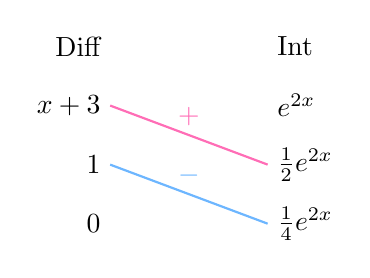
\begin{tikzpicture}[yscale=0.75]
      \draw (-1, 1) node[left]{Diff};
      \draw (1,  1) node[right]{Int};
      \draw (-1, -0) node[left]{$x+3$};
      \draw (1,  -0) node[right]{$e^{2x}$};
      \draw (-1, -1) node[left]{$1$};
      \draw (-1, -2) node[left]{$0$};
      \draw (1,  -1) node[right]{$\frac{1}{2}e^{2x}$};
      \draw (1,  -2) node[right]{$\frac{1}{4}e^{2x}$};
      \draw[thick, M4, -] (-1, -0)--(1, -1); \draw[M4] (0, -0.5) node[above]{$+$};
      \draw[thick, C4, -] (-1, -1)--(1, -2); \draw[C4] (0, -1.5) node[above]{$-$};
    \end{tikzpicture}
  \end{minipage}
  \hspace{5mm}
  \begin{minipage}{0.5\textwidth}
     $\ds\int (x + 3)\,e^{2x}\,\text{d}x = (x + 3)\,\frac{1}{2}e^{2x} - \frac{1}{4}e^{2x}$
  \end{minipage}
\end{sol}

\begin{ex}
  求 $\ds\int (x^2 - 2x)\,e^{kx}\,\text{d}x$. 
\end{ex}

\begin{sol} 
  \begin{minipage}{0.35\textwidth}
    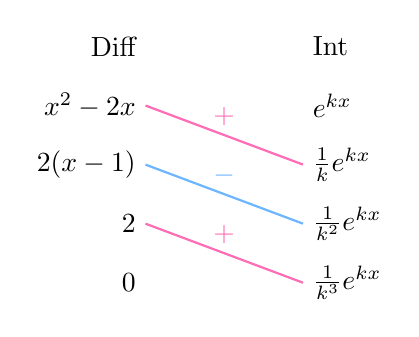
\begin{tikzpicture}[yscale=0.75]
      \draw (-1, 1) node[left]{Diff};
      \draw (1,  1) node[right]{Int};
      \draw (-1, -0) node[left]{$x^2 - 2x$};
      \draw (1,  -0) node[right]{$e^{kx}$};
      \draw (-1, -1) node[left]{$2(x - 1)$};
      \draw (-1, -2) node[left]{$2$};
      \draw (-1, -3) node[left]{$0$};
      \draw (1,  -1) node[right]{$\frac{1}{k}e^{kx}$};
      \draw (1,  -2) node[right]{$\frac{1}{k^2}e^{kx}$};
      \draw (1,  -3) node[right]{$\frac{1}{k^3}e^{kx}$};
      \draw[thick, M4, -] (-1, -0)--(1, -1); \draw[M4] (0, -0.5) node[above]{$+$};
      \draw[thick, C4, -] (-1, -1)--(1, -2); \draw[C4] (0, -1.5) node[above]{$-$};
      \draw[thick, M4, -] (-1, -2)--(1, -3); \draw[M4] (0, -2.5) node[above]{$+$};
    \end{tikzpicture}
  \end{minipage}
  \hspace{5mm}
  \begin{minipage}{0.6\textwidth}
    $\ds\int (x^2 - 2x)\,e^{kx}\,\text{d}x = (x^2 - 2x)\,\frac{1}{k}e^{kx} - 2(x-1)\frac{1}{k^2}e^{kx} + 2\frac{1}{k^3}e^{kx}$
  \end{minipage}
\end{sol}

\begin{ex}
  求 $\ds\int x^4\,\sin 2x\,\text{d}x$. 
\end{ex}

\begin{sol} 
  \begin{minipage}{0.25\textwidth}
    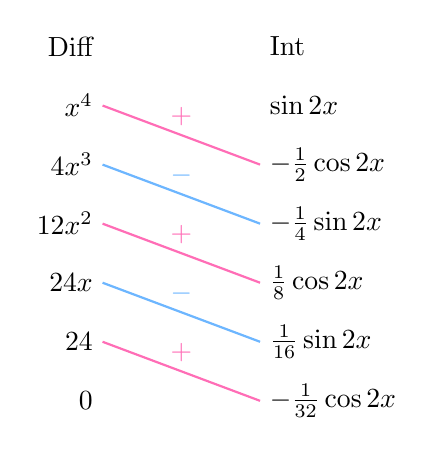
\begin{tikzpicture}[yscale=0.75]
      \draw (-1, 1) node[left]{Diff};
      \draw (1,  1) node[right]{Int};
      \draw (-1, -0) node[left]{$x^4$};
      \draw (1,  -0) node[right]{$\sin 2x$};
      \draw (-1, -1) node[left]{$4x^3$};
      \draw (-1, -2) node[left]{$12x^2$};
      \draw (-1, -3) node[left]{$24x$};
      \draw (-1, -4) node[left]{$24$};
      \draw (-1, -5) node[left]{$0$};
      \draw (1,  -1) node[right]{$-\frac{1}{2}\cos 2x$};
      \draw (1,  -2) node[right]{$-\frac{1}{4}\sin 2x$};
      \draw (1,  -3) node[right]{$\frac{1}{8}\cos 2x$};
      \draw (1,  -4) node[right]{$\frac{1}{16}\sin 2x$};
      \draw (1,  -5) node[right]{$-\frac{1}{32}\cos 2x$};
      \draw[thick, M4, -] (-1, -0)--(1, -1); \draw[M4] (0, -0.5) node[above]{$+$};
      \draw[thick, C4, -] (-1, -1)--(1, -2); \draw[C4] (0, -1.5) node[above]{$-$};
      \draw[thick, M4, -] (-1, -2)--(1, -3); \draw[M4] (0, -2.5) node[above]{$+$};
      \draw[thick, C4, -] (-1, -3)--(1, -4); \draw[C4] (0, -3.5) node[above]{$-$};
      \draw[thick, M4, -] (-1, -4)--(1, -5); \draw[M4] (0, -4.5) node[above]{$+$};
    \end{tikzpicture}
  \end{minipage}
  \hspace{5mm}
  \begin{minipage}{0.7\textwidth}
    $\ds\int x^4\,\sin 2x\,\text{d}x \\= -x^4\,\frac{1}{2}\cos 2x + 4x^3\,\frac{1}{4}\sin 2x + 12x^2\,\frac{1}{8}\cos 2x - 24x\,\frac{1}{16}\sin 2x - 24\,\frac{1}{32}\cos 2x \\= \bigg(-\frac{x^4}{2} + \frac{3x^2}{2} - \frac{3}{4}\bigg)\cos 2x\,+\,\bigg(x^3-\frac{3x}{2}\bigg)\sin 2x$
  \end{minipage}
\end{sol}

\begin{ex}
  求 $\ds\int x^5\,e^{ax}\,\text{d}x$. 
\end{ex}

\begin{sol} 
  \begin{minipage}{0.3\textwidth}
    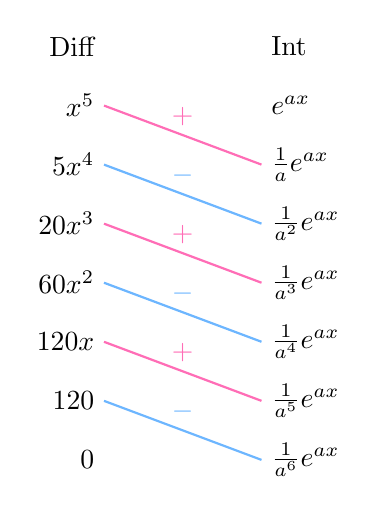
\begin{tikzpicture}[yscale=0.75]
      \draw (-1, 1) node[left]{Diff};
      \draw (1,  1) node[right]{Int};
      \draw (-1, -0) node[left]{$x^5$};
      \draw (1,  -0) node[right]{$e^{ax}$};
      \draw (-1, -1) node[left]{$5x^4$};
      \draw (-1, -2) node[left]{$20x^3$};
      \draw (-1, -3) node[left]{$60x^2$};
      \draw (-1, -4) node[left]{$120x$};
      \draw (-1, -5) node[left]{$120$};
      \draw (-1, -6) node[left]{$0$};
      \draw (1,  -1) node[right]{$\frac{1}{a}e^{ax}$};
      \draw (1,  -2) node[right]{$\frac{1}{a^2}e^{ax}$};
      \draw (1,  -3) node[right]{$\frac{1}{a^3}e^{ax}$};
      \draw (1,  -4) node[right]{$\frac{1}{a^4}e^{ax}$};
      \draw (1,  -5) node[right]{$\frac{1}{a^5}e^{ax}$};
      \draw (1,  -6) node[right]{$\frac{1}{a^6}e^{ax}$};
      \draw[thick, M4, -] (-1, -0)--(1, -1); \draw[M4] (0, -0.5) node[above]{$+$};
      \draw[thick, C4, -] (-1, -1)--(1, -2); \draw[C4] (0, -1.5) node[above]{$-$};
      \draw[thick, M4, -] (-1, -2)--(1, -3); \draw[M4] (0, -2.5) node[above]{$+$};
      \draw[thick, C4, -] (-1, -3)--(1, -4); \draw[C4] (0, -3.5) node[above]{$-$};
      \draw[thick, M4, -] (-1, -4)--(1, -5); \draw[M4] (0, -4.5) node[above]{$+$};
      \draw[thick, C4, -] (-1, -5)--(1, -6); \draw[C4] (0, -5.5) node[above]{$-$};
    \end{tikzpicture}
  \end{minipage}
  \hspace{5mm}
  \begin{minipage}{0.65\textwidth}
    $\ds\int x^5\,e^{ax}\,\text{d}x \\ = x^5\,\frac{1}{a}e^{ax} - 5x^4\,\frac{1}{a^2}e^{ax} + 20x^3\,\frac{1}{a^3}e^{ax} - 60x^2\,\frac{1}{a^4}e^{ax} + 120x\,\frac{1}{a^5}e^{ax} - 120\,\frac{1}{a^6}e^{ax} \\ = \bigg(\frac{x^5}{a}-\frac{5x^4}{a^2} + \frac{20x^3}{a^3} - \frac{60x^2}{a^4} + \frac{120x}{a^5} - \frac{120}{a^6}\bigg)\,e^{ax}$
  \end{minipage}
\end{sol}

\begin{ex}
  求 $\ds\int(\sin^{-1} x)^2\,\text{d}x$. 
\end{ex}

\begin{sol} 
  \begin{minipage}{0.35\textwidth}
    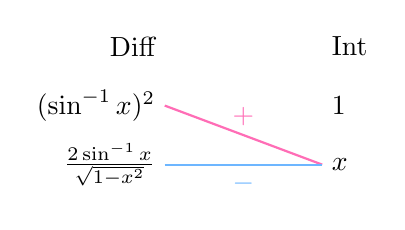
\begin{tikzpicture}[yscale=0.75]
      \draw (-1, 1) node[left]{Diff};
      \draw (1,  1) node[right]{Int};
      \draw (-1, -0) node[left]{$(\sin^{-1} x)^2$};
      \draw (1,  -0) node[right]{$1$};
      \draw (-1, -1) node[left]{$\frac{2\sin^{-1} x}{\sqrt{1-x^2}}$};
      \draw (1,  -1) node[right]{$x$};
      \draw[thick, M4, -] (-1, -0)--(1, -1); \draw[M4] (0, -0.5) node[above]{$+$};
      \draw[thick, C4, -] (-1, -1)--(1, -1); \draw[C4] (0, -1) node[below]{$-$};
    \end{tikzpicture}
    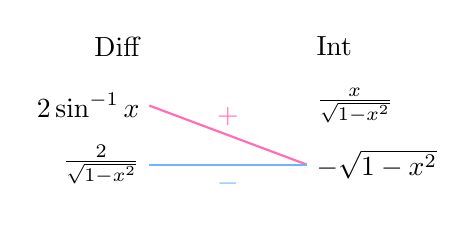
\begin{tikzpicture}[yscale=0.75]
      \draw (-1, 1) node[left]{Diff};
      \draw (1,  1) node[right]{Int};
      \draw (-1, -0) node[left]{$2\sin^{-1} x$};
      \draw (1,  -0) node[right]{$\frac{x}{\sqrt{1-x^2}}$};
      \draw (-1, -1) node[left]{$\frac{2}{\sqrt{1-x^2}}$};
      \draw (1,  -1) node[right]{$-\sqrt{1 - x^2}$};
      \draw[thick, M4, -] (-1, -0)--(1, -1); \draw[M4] (0, -0.5) node[above]{$+$};
      \draw[thick, C4, -] (-1, -1)--(1, -1); \draw[C4] (0, -1) node[below]{$-$};
    \end{tikzpicture}
  \end{minipage}
  \hspace{5mm}
  \begin{minipage}{0.6\textwidth}
    $\ds\int(\sin^{-1} x)^2\,\text{d}x = (\sin^{-1} x)^2\cdot x - \int\!\frac{2\sin^{-1} x}{\sqrt{1-x^2}}\cdot x\,\text{d}x \\= (\sin^{-1} x)^2\cdot x - \int\!2\sin^{-1} x\cdot\frac{x}{\sqrt{1-x^2}}\,\text{d}x \\= (\sin^{-1} x)^2\cdot x - \bigg(-2\sin^{-1} x\cdot\sqrt{1-x^2} + \int\!\frac{2}{\sqrt{1-x^2}}\cdot\sqrt{1-x^2}\,\text{d}x\bigg)\\ = (\sin^{-1} x)^2\cdot x + 2\sin^{-1} x\cdot\sqrt{1-x^2} - 2x$
  \end{minipage}
\end{sol}

\begin{ex}
  求 $\ds\int\!e^{ax}\cos bx\,\text{d}x$, $a$, $b\ne 0$. 
\end{ex}

\begin{sol} 
  \begin{minipage}{0.35\textwidth}
    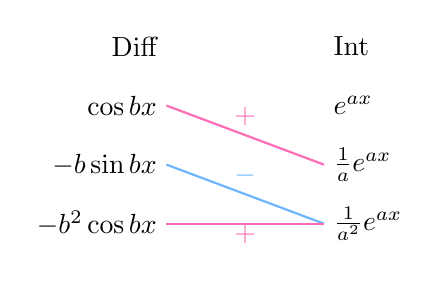
\begin{tikzpicture}[yscale=0.75]
      \draw (-1, 1) node[left]{Diff};
      \draw (1,  1) node[right]{Int};
      \draw (-1, -0) node[left]{$\cos bx$};
      \draw (1,  -0) node[right]{$e^{ax}$};
      \draw (-1, -1) node[left]{$-b\sin bx$};
      \draw (-1, -2) node[left]{$-b^2\cos bx$};
      \draw (1,  -1) node[right]{$\frac{1}{a}e^{ax}$};
      \draw (1,  -2) node[right]{$\frac{1}{a^2}e^{ax}$};
      \draw[thick, M4, -] (-1, -0)--(1, -1); \draw[M4] (0, -0.5) node[above]{$+$};
      \draw[thick, C4, -] (-1, -1)--(1, -2); \draw[C4] (0, -1.5) node[above]{$-$};
      \draw[thick, M4, -] (-1, -2)--(1, -2); \draw[M4] (0, -2.5) node[above]{$+$};
    \end{tikzpicture}
  \end{minipage}
  \hspace{5mm}
  \begin{minipage}{0.6\textwidth}
    $\ds\int\!e^{ax}\cos bx\,\text{d}x = \frac{1}{a}e^{ax}\cos bx + \frac{b}{a^2}e^{ax}\sin bx - \frac{b^2}{a^2}\int\!e^{ax}\cos bx\,\text{d}x\\ \ie\int\!e^{ax}\cos bx\,\text{d}x = \frac{e^{ax}(a\cos bx + b\sin bx)}{a^2 + b^2}$
  \end{minipage}
\end{sol}

\begin{ex}
  求 $\ds\int\!e^{ax}\sin bx\,\text{d}x$, $a$, $b\ne 0$. 
\end{ex}

\begin{sol} 
  \begin{minipage}{0.35\textwidth}
    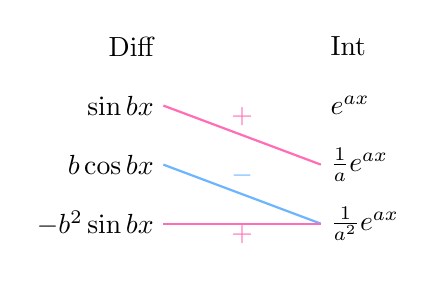
\begin{tikzpicture}[yscale=0.75]
      \draw (-1, 1) node[left]{Diff};
      \draw (1,  1) node[right]{Int};
      \draw (-1, -0) node[left]{$\sin bx$};
      \draw (1,  -0) node[right]{$e^{ax}$};
      \draw (-1, -1) node[left]{$b\cos bx$};
      \draw (-1, -2) node[left]{$-b^2\sin bx$};
      \draw (1,  -1) node[right]{$\frac{1}{a}e^{ax}$};
      \draw (1,  -2) node[right]{$\frac{1}{a^2}e^{ax}$};
      \draw[thick, M4, -] (-1, -0)--(1, -1); \draw[M4] (0, -0.5) node[above]{$+$};
      \draw[thick, C4, -] (-1, -1)--(1, -2); \draw[C4] (0, -1.5) node[above]{$-$};
      \draw[thick, M4, -] (-1, -2)--(1, -2); \draw[M4] (0, -2.5) node[above]{$+$};
    \end{tikzpicture}
  \end{minipage}
  \hspace{5mm}
  \begin{minipage}{0.6\textwidth}
    $\ds\int\!e^{ax}\sin bx\,\text{d}x = \frac{1}{a}e^{ax}\sin bx - \frac{b}{a^2}e^{ax}\cos bx - \frac{b^2}{a^2}\int\!e^{ax}\sin bx\,\text{d}x\\ \ie\int\!e^{ax}\sin bx\,\text{d}x = \frac{e^{ax}(a\sin bx - b\cos bx)}{a^2 + b^2}$
  \end{minipage}
\end{sol}

\myline

\subsubsection*{遞迴式}
\begin{ex} 
  令 $\ds I_n = \int\!\frac{1}{(x^2 + a^2)^n}\,\text{d}x$, $n\in\mathbb{N}$, 則 $\ds I_{n + 1} = \frac{x}{2na^2(x^2 + a^2)^n} + \frac{2n - 1}{2na^2}I_n$.
\end{ex}

\begin{sol}
  令 $\ds u = \frac{1}{(x^2 + a^2)^n}$, 則 $\ds\text{d}u = -2n\,\frac{x}{(x^2 + a^2)^{n + 1}}\,\text{d}x$; $\ds\text{d}v = \text{d}x$, 則 $\ds v = x$. 故 $\ds I_n = \int\!\frac{1}{(x^2 + a^2)^n}\,\text{d}x = \frac{x}{(x^2 + a^2)^n} + 2n\int\!\frac{x^2}{(x^2 + a^2)^{n + 1}}\,\text{d}x = \frac{x}{(x^2 + a^2)^n} + 2n\int\frac{(x^2 + a^2 - a^2)}{(x^2 + a^2)^{n + 1}}\,\text{d}x = \frac{x}{(x^2 + a^2)^n} + 2n I_n - 2na^2 I_{n + 1}\ie 2na^2 I_{n + 1} = \frac{x}{(x^2 + a^2)^n} + (2n - 1)I_n\ie I_{n + 1} = \frac{x}{2na^2(x^2 + a^2)^n} + \frac{2n - 1}{2na^2}I_n$.  
\end{sol}

\begin{rmk}[使用例]
  $\ds I_1 = \frac{1}{a}\tan^{-1}\frac{x}{a}$, $\ds I_2 = \frac{1}{2a^2}\,I_1 + \frac{x}{2a^2(x^2+a^2)} = \frac{1}{2a^3}\tan^{-1}\frac{x}{a} + \frac{x}{2a^2(x^2+a^2)}$, $\ds I_3 = \frac{3}{4a^2}\,I_2 + \frac{x}{4a^2(x^2+a^2)^2} = \frac{3}{4a^2}\bigg(\frac{1}{2a^3}\tan^{-1}\frac{x}{a} + \frac{x}{2a^2(x^2+a^2)}\bigg) + \frac{x}{4a^2(x^2+a^2)^2} = \frac{3}{8a^5}\tan^{-1}\frac{x}{a} + \frac{3x}{8a^4(x^2+a^2)} + \frac{x}{4a^2(x^2+a^2)^2}$.
\end{rmk}

\begin{ex} 
  令 $\ds J_n = \int\!\sin^n\!x\,\text{d}x$, $n\in\mathbb{N}$, $n\geqslant 2$, 則 $\ds J_n = \frac{-\sin^{n - 1}\!x\cos x}{n} + \frac{n - 1}{n}\,J_{n - 2}$. 
\end{ex}

\begin{sol}
  令 $\ds u = \sin^{n-1}\!x$, 則 $\ds\text{d}u = (n - 1)\,\sin^{n - 2}\!x\,\cos x\,\text{d}x$; $\ds\text{d}v = \sin x\,\text{d}x$, 則 $\ds v = -\cos x$. 故 $\ds J_n = \int\!\sin^n\!x\,\text{d}x = -\sin^{n - 1}\!x\cdot\cos x + (n - 1)\,\int\!\cos x\cdot\sin^{n - 2}\!x\cos x\,\text{d}x = -\sin^{n - 1}\!x\cos x + (n - 1)\,\int\!\sin^{n - 2}\!x\cos^2\!x\,\text{d}x = -\sin^{n - 1}\!x\cos x + (n - 1)\,\int\!\sin^{n - 2}\!x\cdot(1 - \sin^2\!x)\,\text{d}x = -\sin^{n - 1}\!x\cos x + (n - 1)\,\int\!\sin^{n - 2}\!x\,\text{d}x - (n - 1)\,\int\!\sin^n\!x\,\text{d}x = -\sin^{n - 1}\!x\cos x + (n - 1) J_{n - 2} + (1 - n)J_n\ie n J_n = -\sin^{n - 1}\!x\cos x + (n - 1) J_{n - 2} \ie J_n = \frac{-\sin^{n - 1}\!x\cos x}{n} + \frac{n - 1}{n}\,J_{n - 2}$.  
\end{sol}

\begin{rmk}[使用例]
  $\ds J_2 = \frac{-\sin x\cos x}{2} + \frac{1}{2}\,J_0 = \frac{-\sin x\cos x}{2} + \frac{x}{2}$, $\ds J_3 = \frac{-\sin^2\!x\cos x}{3} + \frac{2}{3}\,J_1 = \frac{-\sin^2\!x\cos x}{3} - \frac{2\cos x}{3}$, $\ds J_4 = \frac{-\sin^3\!x\cos x}{4} + \frac{3}{4}\,J_2 = \frac{-\sin^3\!x\cos x}{4} + \frac{3\sin x\cos x}{8} - \frac{3x}{8}$.
\end{rmk}

\begin{ex} 
  令 $\ds K_n = \int\!\sec^{2n+1}\!\theta\,\text{d}\theta$, $n\in\mathbb{N}$, $n\geqslant 1$, 則 $\ds K_n = \frac{\sec^{2n - 1}\theta\tan\theta}{2n} + \frac{2n - 1}{2n}\,K_{n - 1}$. 
\end{ex}

\begin{sol}
  令 $\ds u = \sec^{2n - 1}\!\theta$, 則 $\ds\text{d}u = (2n - 1)\sec^{2n - 2}\theta\cdot\sec\theta\tan\theta\,\text{d}\theta = (2n - 1)\sec^{2n - 1}\theta\tan\theta\,\text{d}\theta$; 令 $\ds\text{d}v = \sec^2\theta\,\text{d}\theta$, 則 $\ds v = \tan\theta$. 故 $\ds K_n = \int\!\sec^{2n + 1}\!\theta\,\text{d}\theta = \sec^{2n - 1}\!\theta\cdot\tan\theta - \int\!\tan\theta\cdot(2n - 1)\sec^{2n - 1}\theta\tan\theta\,\text{d}\theta = \sec^{2n -1}\!\theta\tan\theta - (2n - 1)\int\!\tan^2\theta\cdot\sec^{2n - 1}\theta\,\text{d}\theta = \sec^{2n - 1}\!\theta\tan\theta - (2n - 1)\int\!(\sec^2\theta - 1)\cdot\sec^{2n - 1}\!\theta\,\text{d}\theta = \sec^{2n - 1}\!\theta\tan\theta - (2n - 1)\int\!\sec^{2n + 1}\theta\,\text{d}\theta + (2n - 1)\int\!\sec^{2 n - 1}\!\theta\,\text{d}\theta \ie K_n = \sec^{2n - 1}\!\theta\tan\theta - (2n - 1)K_n + (2n - 1)K_{n - 1} \ie K_n = \frac{\sec^{2n - 1}\!\theta\tan\theta}{2n} + \frac{2n - 1}{2n}K_{n - 1}$.
\end{sol}

\begin{rmk}[使用例]
  $\ds K_0 = \int\!\sec\theta\,\text{d}\theta = \ln|\sec\theta + \tan\theta|$, $\ds\int\!\sec^3\!\theta\,\text{d}\theta = K_1 = \frac{\sec\theta\tan\theta}{2} + \frac{1}{2}\,K_0 = \frac{1}{2}\,\big(\sec\theta\tan\theta + \ln|\sec\theta + \tan\theta|\big)$, $\ds \int\!\sec^5\!\theta\,\text{d}\theta = K_2 = \frac{\sec^3\!\theta\tan\theta}{4} + \frac{3}{4}\,K_1 = \frac{\sec^3\!\theta\tan\theta}{4} + \frac{3}{8}\,\big(\sec\theta\tan\theta + \ln|\sec\theta + \tan\theta|\big)$. 
\end{rmk}

\myline

\begin{exe} 以部份積分法求下列不定積分. 注意: 可能會因為常數項而跟此處答案不同.
  %\setlength{\columnsep}{-2cm}
  \begin{multicols}{3}
    \begin{enumerate}\setlength{\itemsep}{0pt}
      \item $\ds\int\frac{\sin^{-1}x}{x^2}\,\text{d}x $%{\color{C2}\;= - \frac{\sin^{-1}x}{x} - \ln\Big|\frac{1 - \sqrt{1 - x^2}}{x}\Big| + c}$
      \item $\ds\int\ln(x + \sqrt{1 + x^2})\,\text{d}x $%{\color{C2}\;= x\,\ln(x + \sqrt{1 + x^2}) - \sqrt{1 + x^2} + c}$
      \item $\ds\int x^3\ln x\,\text{d}x $%{\color{C2}\;= \frac{x^4}{4}\ln x -\frac{x^4}{16} + c}$
      \item $\ds\int x(\ln x)^3\,\text{d}x $%{\color{C2}\;= \frac{x^2}{2}\Big((\ln x)^3 -\frac{3(\ln x)^2}{2} + \frac{3\ln x}{2} - \frac{3}{4} \Big) + c}$
      \item $\ds\int x^2\tan^{-1} x\,\text{d}x $%{\color{C2}\;= \frac{x^3}{3}\tan^{-1} x - \frac{x^2}{6} + \frac{\ln(1 + x^2)}{6} + c}$
      \item $\ds\int\!\frac{x e^x}{(x + 1)^2}\,\text{d}x $%{\color{C2}\;= \frac{e^x}{x + 1} + c}$
      \item $\ds\int x^5 e^{-x^2}\,\text{d}x $%{\color{C2}\;= -\frac{1}{2}e^{-x^2}(x^4 + 2x^2 + 2) + c}$
      \item $\ds\int x e^{\sqrt{x}}\,\text{d}x $%{\color{C2}\;= 2\,e^{\sqrt{x}}\,\big(x\sqrt{x} - 3x + 6\sqrt{x} - 6\big) + c}$
      %\item $\ds\int(\sin^{-1} x)^2\,\text{d}x $%{\color{C2}\;= x\,(\sin^{-1} x)^2 + 2\sqrt{1 - x^2}\,\sin^{-1} x - 2x + c}$
      \item $\ds\int(2x^2 + 1)e^{x^2}\,\text{d}x$%{\color{C2}\;= xe^{x^2}$
      \item $\ds\int\!\sin(\ln x)\,\text{d}x $%{\color{C2}\;= \frac{x\,(\sin(\ln x) - \cos(\ln x))}{2} + c}$
      \item $\ds\int\!x^2\ln\frac{1 - x}{1 + x}\,\text{d}x $%{\color{C2}\;= \frac{x^3}{3}\ln\frac{1 - x}{1 + x} - \frac{x^2 + \ln(x^2 - 1)}{3} + c}$
      \item $\ds\int\!\frac{\ln x}{\sqrt{1 + x}}\,\text{d}x $%{\color{C2}\;= \ln x\cdot 2\sqrt{1 + x} - 4\sqrt{1+x} - 2\ln(\sqrt{1 + x}-1) + 2\ln(\sqrt{1+x} + 1) + c}$
    \end{enumerate}
  \end{multicols}
\end{exe}

\begin{sol}
  \begin{enumerate}\setlength{\itemsep}{0pt}
    \item[]
    \item 令 $\ds u = \sin^{-1}x$, 則 $\ds\text{d}u = \frac{1}{\sqrt{1 - x^2}}\,\text{d}x$; $\ds\text{d}v = \frac{1}{x^2}\,\text{d}x$, 則 $\ds v = \frac{-1}{x}$. 故 $\ds\int\frac{\sin^{-1}x}{x^2}\,\text{d}x = \sin^{-1}x\cdot\frac{-1}{x} - \int\!\frac{-1}{x}\cdot\frac{1}{\sqrt{1 - x^2}}\,\text{d}x = -\frac{\sin^{-1}x}{x} + \int\!\frac{1}{x\sqrt{1 - x^2}}\,\text{d}x$. 令 $\ds w = \sqrt{1 - x^2}$, 則 $-x^2 = w^2 - 1$, $\ds\text{d}w = \frac{-x}{\sqrt{1 - x^2}}\,\text{d}x$. 故 $\ds\int\!\frac{1}{x\sqrt{1 - x^2}}\,\text{d}x = \int\!\frac{1}{-x^2}\cdot\frac{-x}{\sqrt{1 - x^2}}\,\text{d}x = \int\frac{1}{w^2 - 1}\,\text{d}w = \frac{1}{2}\int\Big(\frac{1}{w - 1} - \frac{1}{w + 1}\Big)\,\text{d}w = \frac{1}{2}\big(\ln|w - 1| - \ln|w + 1|\big) = \frac{1}{2}\ln\Big|\frac{w - 1}{w + 1}\Big| = \frac{1}{2}\ln\bigg|\frac{\sqrt{1 - x^2} - 1}{\sqrt{1 - x^2} + 1}\bigg| = \frac{1}{2}\ln\bigg|\frac{1 - \sqrt{1 - x^2}}{1 + \sqrt{1 - x^2}}\bigg| = \frac{1}{2}\ln\bigg|\frac{1 - \sqrt{1 - x^2}}{1 + \sqrt{1 - x^2}}\cdot\frac{1 - \sqrt{1 - x^2}}{1 - \sqrt{1 - x^2}}\bigg| = \frac{1}{2}\ln\bigg|\frac{(1 - \sqrt{1 - x^2})^2}{x^2}\bigg| = \ln\bigg|\frac{1 - \sqrt{1 - x^2}}{x}\bigg|$. \\以上, $\ds\int\frac{\sin^{-1}x}{x^2}\,\text{d}x = - \frac{\sin^{-1}x}{x} + \int\!\frac{1}{x\sqrt{1 - x^2}}\,\text{d}x = - \frac{\sin^{-1}x}{x} + \ln\bigg|\frac{1 - \sqrt{1 - x^2}}{x}\bigg| + c$.
    \item 令 $\ds u = \ln(x + \sqrt{1 + x^2})$, 則 $\ds\text{d}u = \frac{1}{x + \sqrt{1 + x^2}}\cdot\big(x + \sqrt{1 + x^2}\big)'\,\text{d}x = \frac{1}{x + \sqrt{1 + x^2}}\cdot\Big(1 + \frac{x}{\sqrt{1 + x^2}}\Big)\,\text{d}x = \frac{1}{\sqrt{1 + x^2}}\,\text{d}x$; $\ds\text{d}v = \text{d}x$, 則 $\ds v = x$. 故 $\ds\int\ln(x + \sqrt{1 + x^2})\,\text{d}x = \ln(x + \sqrt{1 + x^2})\cdot x - \int\!x\cdot\frac{1}{\sqrt{1 + x^2}}\,\text{d}x = \ln(x + \sqrt{1 + x^2})\,x - \sqrt{1 + x^2} + c$.
    \item 令 $\ds u = \ln x$, 則 $\ds\text{d}u = \frac{1}{x}\,\text{d}x$; $\ds\text{d}v = x^3\,\text{d}x$, 則 $\ds v = \frac{x^4}{4}$.  故 $\ds\int x^3\ln x\,\text{d}x = \ln x\cdot\frac{x^4}{4} - \int\!\frac{x^4}{4}\cdot\frac{1}{x}\,\text{d}x = \ln x\cdot\frac{x^4}{4} - \int\!\frac{x^3}{4}\,\text{d}x = \ln x\cdot\frac{x^4}{4} - \frac{x^4}{16} + c$.   
    \item 令 $\ds u = (\ln x)^3$, 則 $\ds\text{d}u = 3(\ln x)^2\cdot\frac{1}{x}\,\text{d}x$; $\ds\text{d}v = x\,\text{d}x$, 則 $\ds v = \frac{x^2}{2}$.  故 $\ds\int x(\ln x)^3\,\text{d}x = (\ln x)^3\cdot\frac{x^2}{2} - \int\!\frac{x^2}{2}\cdot 3(\ln x)^2\cdot\frac{1}{x}\,\text{d}x = (\ln x)^3\cdot\frac{x^2}{2} - \frac{3}{2}\int x(\ln x)^2\,\text{d}x$. 令 $\ds u = (\ln x)^2$, 則 $\ds\text{d}u = 2\,\ln x\cdot\frac{1}{x}\,\text{d}x$; $\ds\text{d}v = x\,\text{d}x$, 則 $\ds v = \frac{x^2}{2}$.  故 $\ds\int x(\ln x)^2\,\text{d}x = (\ln x)^2\cdot\frac{x^2}{2} - \int\!\frac{x^2}{2}\cdot 2\ln x\cdot\frac{1}{x}\,\text{d}x = (\ln x)^2\cdot\frac{x^2}{2} - \int x\ln x\,\text{d}x$. 令 $\ds u = \ln x$, 則 $\ds\text{d}u = \frac{1}{x}\,\text{d}x$; $\ds\text{d}v = x\,\text{d}x$, 則 $\ds v = \frac{x^2}{2}$. 故 $\ds\int x\ln x\,\text{d}x = \ln x\cdot\frac{x^2}{2} - \int\!\frac{x^2}{2}\cdot\frac{1}{x}\,\text{d}x = \ln x\cdot\frac{x^2}{2} - \frac{1}{2}\int x\,\text{d}x = \ln x\cdot\frac{x^2}{2} - \frac{x^2}{4}$. 以上, $\ds\int x(\ln x)^3\,\text{d}x = (\ln x)^3\cdot\frac{x^2}{2} - \frac{3}{2}\Big((\ln x)^2\cdot\frac{x^2}{2} - \big(\ln x\cdot\frac{x^2}{2} - \frac{x^2}{4}\big)\Big) = \frac{x^2}{2}\big((\ln x)^3 - \frac{3(\ln x)^2}{2} + \frac{3\ln x}{2} - \frac{3}{4}\big) + c$
    \item 令 $\ds u = \tan^{-1} x$, 則 $\ds\text{d}u = \frac{1}{1 + x^2}\,\text{d}x$; $\ds\text{d}v = x^2\,\text{d}x$, 則 $\ds v = \frac{x^3}{3}$.  故 $\ds\int x^2\tan^{-1} x\,\text{d}x = \tan^{-1}x\cdot\frac{x^3}{3} - \int\!\frac{x^3}{3}\cdot\frac{1}{x^2 + 1}\,\text{d}x$. 又 $\ds\int\!\frac{x^3}{3}\cdot\frac{1}{x^2 + 1}\,\text{d}x = \frac{1}{3}\int\!\frac{(x^3 + x) - x}{x^2 + 1}\,\text{d}x = \frac{1}{3}\int\!\frac{x(x^2 + 1) - x}{x^2 + 1}\,\text{d}x = \frac{1}{3}\int\!\big(x - \frac{x}{x^2 + 1}\big)\,\text{d}x$. 令 $\ds w = x^2 + 1$, 則 $\ds\text{d}w = 2x\,\text{d}x\ie x\,\text{d}x = \frac{1}{2}\,\text{d}w$, 故 $\ds\int\!\frac{x}{x^2 + 1}\,\text{d}x = \int\!\frac{1}{x^2 + 1}\cdot x\,\text{d}x = \int\!\frac{1}{w}\cdot\frac{1}{2}\,\text{d}w = \frac{1}{2}\ln w + c = \frac{1}{2}\ln(x^2 + 1) + c$. 以上, $\ds\int x^2\tan^{-1} x\,\text{d}x = \tan^{-1}x\cdot\frac{x^3}{3} - \int\!\frac{x^3}{3}\cdot\frac{1}{x^2 + 1}\,\text{d}x = \tan^{-1}x\cdot\frac{x^3}{3} - \frac{x^2}{6} + \frac{\ln(x^2 + 1)}{6} + c$. 
    \item $\ds\int\!\frac{x e^x}{(x + 1)^2}\,\text{d}x = \int\!\frac{(x + 1 - 1)e^x}{(x + 1)^2}\,\text{d}x = \int\!\frac{e^x}{x + 1}\,\text{d}x - \int\!\frac{e^x}{(x + 1)^2}\,\text{d}x$. 令 $\ds u = e^x$, 則 $\ds\text{d}u = e^x\,\text{d}x$; $\ds\text{d}v = \frac{1}{(x + 1)^2}\,\text{d}x$, 則 $\ds v = \frac{-1}{x + 1}$. 故 $\ds\int\!\frac{e^x}{(x + 1)^2}\,\text{d}x = e^x\cdot\frac{-1}{x + 1} + \int\!\frac{1}{x + 1}\cdot e^x\,\text{d}x = \frac{-e^x}{x + 1} + \int\!\frac{e^x}{x + 1}\,\text{d}x$; 原式 $\ds\int\!\frac{x e^x}{(x + 1)^2}\,\text{d}x = \int\!\frac{e^x}{x + 1}\,\text{d}x - \int\!\frac{e^x}{(x + 1)^2}\,\text{d}x = \int\!\frac{e^x}{x + 1}\,\text{d}x - \Big(\frac{-e^x}{x + 1} + \int\!\frac{e^x}{x + 1}\,\text{d}x\Big) = \frac{e^x}{x + 1}$. 
    \item 令 $\ds w = x^2$, 則 $\ds\text{d}w = 2x\,\text{d}x\ie x\,\text{d}x = \frac{1}{2}\,\text{d}w$, 故 $\ds\int x^5 e^{-x^2}\,\text{d}x = \int e^{-x^2}\cdot(x^2)^2\cdot x\,\text{d}x = \int e^{-w}\cdot w^2\cdot\frac{1}{2}\,\text{d}w = \frac{1}{2}\int w^2\,e^{-w}\,\text{d}w = -\frac{1}{2}\,e^{-w}(w^2 + 2w + 2) = -\frac{1}{2}\,e^{-x^2}(x^4 + 2x^2 + 2) + c$. \\
  \begin{minipage}{0.15\textwidth}
    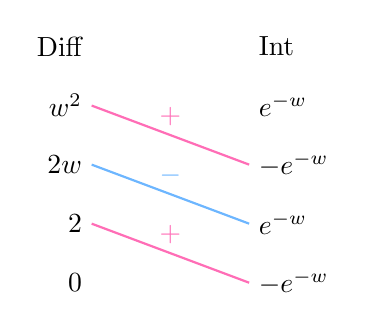
\begin{tikzpicture}[yscale=0.75]
      \draw (-1, 1) node[left]{Diff};
      \draw (1,  1) node[right]{Int};
      \draw (-1, -0) node[left]{$w^2$};
      \draw (1,  -0) node[right]{$e^{-w}$};
      \draw (-1, -1) node[left]{$2w$};
      \draw (-1, -2) node[left]{$2$};
      \draw (-1, -3) node[left]{$0$};
      \draw (1,  -1) node[right]{$-e^{-w}$};
      \draw (1,  -2) node[right]{$e^{-w}$};
      \draw (1,  -3) node[right]{$-e^{-w}$};
      \draw[thick, M4, -] (-1, -0)--(1, -1); \draw[M4] (0, -0.5) node[above]{$+$};
      \draw[thick, C4, -] (-1, -1)--(1, -2); \draw[C4] (0, -1.5) node[above]{$-$};
      \draw[thick, M4, -] (-1, -2)--(1, -3); \draw[M4] (0, -2.5) node[above]{$+$};
    \end{tikzpicture}
  \end{minipage}
  \hspace{5mm}
  \begin{minipage}{0.8\textwidth}
    \begin{align*}
      \int w^2 e^{-w}\,\text{d}w = -w^2\,e^{-w} - 2w\,e^{-w} - 2\,e^{-w} = -e^{-w}(w^2 + 2w + 2)
    \end{align*}
  \end{minipage}
\item 令 $\ds w = \sqrt{x}$, 則 $\ds w^2 = x$, $\ds\text{d}x = 2w\,\text{d}w$, 故 $\ds\int x e^{\sqrt{x}}\,\text{d}x = \int w^2 e^w\cdot 2w\,\text{d}w = 2\int w^3 e^w\,\text{d}w = 2\,e^w(w^3 - 3w^2 + 6w - 6) = 2\,e^{\sqrt{x}}\,(x\sqrt{x} - 3 x + 6\sqrt{x} - 6) + c$ \\ 
  \begin{minipage}{0.15\textwidth}
    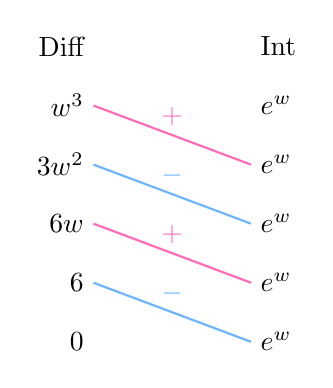
\begin{tikzpicture}[yscale=0.75]
      \draw (-1, 1) node[left]{Diff};
      \draw (1,  1) node[right]{Int};
      \draw (-1, -0) node[left]{$w^3$};
      \draw (1,  -0) node[right]{$e^w$};
      \draw (-1, -1) node[left]{$3w^2$};
      \draw (-1, -2) node[left]{$6w$};
      \draw (-1, -3) node[left]{$6$};
      \draw (-1, -4) node[left]{$0$};
      \draw (1,  -1) node[right]{$e^w$};
      \draw (1,  -2) node[right]{$e^w$};
      \draw (1,  -3) node[right]{$e^w$};
      \draw (1,  -4) node[right]{$e^w$};
      \draw[thick, M4, -] (-1, -0)--(1, -1); \draw[M4] (0, -0.5) node[above]{$+$};
      \draw[thick, C4, -] (-1, -1)--(1, -2); \draw[C4] (0, -1.5) node[above]{$-$};
      \draw[thick, M4, -] (-1, -2)--(1, -3); \draw[M4] (0, -2.5) node[above]{$+$};
      \draw[thick, C4, -] (-1, -3)--(1, -4); \draw[C4] (0, -3.5) node[above]{$-$};
    \end{tikzpicture}
  \end{minipage}
  \hspace{5mm}
  \begin{minipage}{0.8\textwidth}
    \begin{align*}
      \int w^3\,e^w\,\text{d}w = w^3\,e^w - 3w^2\,e^w + 6w\,e^w - 6\,e^w = e^w(w^3 - 3w^2 + 6w - 6)
    \end{align*}
  \end{minipage}
    %\item 令 $\ds u = (\sin^{-1} x)^2$, 則 $\ds\text{d}u = 2\sin^{-1}x\frac{1}{\sqrt{1 - x^2}}\,\text{d}x$; $\ds\text{d}v = \text{d}x$, 則 $\ds v = x$.  故 $\ds\int(\sin^{-1} x)^2\,\text{d}x = (\sin^{-1} x)^2\cdot x - \int x\cdot 2\sin^{-1}x\frac{1}{\sqrt{1 - x^2}}\,\text{d}x = (\sin^{-1} x)^2\cdot x + 2\int\!\sin^{-1}x\cdot\frac{-x}{\sqrt{1 - x^2}}\,\text{d}x$. 令 $\ds u = \sin^{-1} x$, 則 $\ds\text{d}u = \frac{1}{\sqrt{1 - x^2}}\,\text{d}x$; $\ds\text{d}v = \frac{-x}{\sqrt{1 - x^2}}\,\text{d}x$, 則 $\ds v = \sqrt{1 - x^2}$.  故 $\ds\int\!\sin^{-1}x\cdot\frac{-x}{\sqrt{1 - x^2}}\,\text{d}x = \sin^{-1}x\cdot\sqrt{1 - x^2} - \int\!\sqrt{1 - x^2}\cdot\frac{1}{\sqrt{1 - x^2}}\,\text{d}x = \sin^{-1}x\cdot\sqrt{1 - x^2} - \int 1\,\text{d}x = \sin^{-1}x\cdot\sqrt{1 - x^2} - x$. 以上, $\ds\int(\sin^{-1} x)^2\,\text{d}x = (\sin^{-1} x)^2\cdot x + 2\,(\sin^{-1}x\cdot\sqrt{1 - x^2} - x) = x\,(\sin^{-1} x)^2 + 2\sqrt{1 - x^2}\,\sin^{-1}x - 2x + c$
    \item $\ds\int(2x^2 + 1)\,e^{x^2}\,\text{d}x = \int\!2x^2\,e^{x^2}\,\text{d}x + \int\!e^{x^2}\,\text{d}x$. 令 $\ds u = x$, 則 $\ds\text{d}u = \text{d}x$; $\ds\text{d}v = 2x\,e^{x^2}\,\text{d}x$, 則 $\ds v = e^{x^2}$. 故 $\ds\int\!2x^2\,e^{x^2}\,\text{d}x = x\cdot e^{x^2} - \int\!e^{x^2}\text{d}x$; 原式 $\ds\int\!2x^2\,e^{x^2}\,\text{d}x + \int\!e^{x^2}\,\text{d}x = x\cdot e^{x^2} - \int\!e^{x^2}\text{d}x + \int\!e^{x^2}\,\text{d}x = xe^{x^2}$
    \item 令 $\ds w = \ln x$, 則 $\ds e^w = x$, $\ds\text{d}x = e^w\,\text{d}w$, 故 $\ds\int\!\sin(\ln x)\,\text{d}x = \int\!\sin w\cdot e^w\,\text{d}w = \int e^w\,\sin w\,\text{d}w = \frac{e^w(\sin w - \cos w)}{2} = \frac{x\,(\sin(\ln x) - \cos(\ln x))}{2} + c$ \\
      \begin{minipage}{0.15\textwidth}
        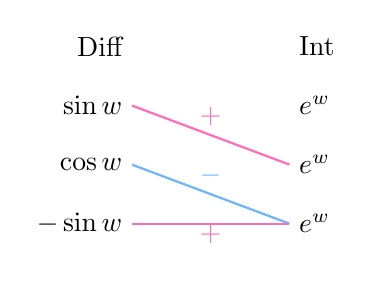
\begin{tikzpicture}[yscale=0.75]
          \draw (-1, 1) node[left]{Diff};
          \draw (1,  1) node[right]{Int};
          \draw (-1, -0) node[left]{$\sin w$};
          \draw (1,  -0) node[right]{$e^w$};
          \draw (-1, -1) node[left]{$\cos w$};
          \draw (-1, -2) node[left]{$-\sin w$};
          \draw (1,  -1) node[right]{$e^w$};
          \draw (1,  -2) node[right]{$e^w$};
          \draw[thick, M4, -] (-1, -0)--(1, -1); \draw[M4] (0, -0.5) node[above]{$+$};
          \draw[thick, C4, -] (-1, -1)--(1, -2); \draw[C4] (0, -1.5) node[above]{$-$};
          \draw[thick, M4, -] (-1, -2)--(1, -2); \draw[M4] (0, -2.5) node[above]{$+$};
        \end{tikzpicture}
      \end{minipage}
      \hspace{5mm}
      \begin{minipage}{0.8\textwidth}
        \begin{align*}
          &\int e^w\sin w\,\text{d}w = e^{w}\sin w - e^w\cos w - \int e^w\sin w\,\text{d}w\\ 
          &\ie\int e^w\sin w\,\text{d}w = \frac{e^w(\sin w - \cos w)}{2}
        \end{align*}
      \end{minipage}

    \item 令 $\ds u = \ln\frac{1 - x}{1 + x}$, 則 $\ds\text{d}u = \frac{1 + x}{1 - x}\cdot\Big(\frac{1 - x}{1 + x}\Big)'\,\text{d}x = \frac{1 + x}{1 - x}\cdot\frac{(1 + x)\cdot(-1)-(1 - x)}{(1 + x)^2}\,\text{d}x = \frac{2}{x^2 - 1}\,\text{d}x$; $\ds\text{d}v = x^2\,\text{d}x$, 則 $\ds v = \frac{x^3}{3}$. 故 $\ds\int\!x^2\ln\frac{1 - x}{1 + x}\,\text{d}x = \ln\frac{1 - x}{1 + x}\cdot\frac{x^3}{3} - \int\frac{x^3}{3}\cdot\frac{2}{x^2 - 1}\,\text{d}x$. 又 $\ds\int\frac{x^3}{3}\cdot\frac{2}{x^2 - 1}\,\text{d}x = \frac{2}{3}\int\!\frac{x^3}{x^2 - 1}\,\text{d}x = \frac{2}{3}\int\!\Big(x + \frac{x}{x^2 - 1}\Big)\,\text{d}x = \frac{x^2}{3} + \frac{2}{3}\int\!\frac{x}{x^2 - 1}\,\text{d}x$. 令 $\ds w = x^2 - 1$, 則 $\ds\text{d}w = 2x\,\text{d}x\ie x\,\text{d}x = \frac{1}{2}\,\text{d}w$, 故 $\ds\int\!\frac{x}{x^2 - 1}\,\text{d}x = \int\!\frac{1}{x^2 - 1}\cdot x\,\text{d}x = \int\!\frac{1}{w}\cdot\frac{1}{2}\,\text{d}w = \frac{1}{2}\ln w + c = \frac{1}{2}\ln(x^2 - 1) + c$. 以上, $\ds\int x^2\ln\frac{1 - x}{1 + x}\,\text{d}x = \frac{1 + x}{1 - x}\cdot\frac{x^3}{3} - \int\!\frac{x^3}{3}\cdot\frac{1}{x^2 - 1}\,\text{d}x = \ln\frac{1 - x}{1 + x}\cdot\frac{x^3}{3} - \frac{x^2 + \ln(x^2 - 1)}{3} + c$. 
    \item 令 $\ds u = \ln x$, 則 $\ds\text{d}u = \frac{1}{x}\,\text{d}x$; $\ds\text{d}v = \frac{1}{\sqrt{1 + x}}\,\text{d}x$, 則 $\ds v = 2\sqrt{1 + x}$. 故 $\ds\int\!\frac{\ln x}{\sqrt{1 + x}}\,\text{d}x = \ln x\cdot 2\sqrt{1 + x} - 2 \int\!\frac{\sqrt{1 + x}}{x}\,\text{d}x$. 令 $\ds w = \sqrt{1 + x}$, 則 $\ds w^2 = 1 + x \ie x= w^2 - 1$, $\ds 2w\,\text{d}w = \text{d}x$, 故 $\ds\int\!\frac{\sqrt{1 + x}}{x}\,\text{d}x = \int\!\frac{w}{w^2 - 1}\cdot 2w\,\text{d}w = 2\int\!\frac{w^2}{w^2 - 1}\,\text{d}w = 2\int\!\frac{(w^2 - 1) + 1}{w^2 - 1}\,\text{d}w = 2 w + 2\int\!\frac{1}{w^2 - 1}\,\text{d}w = 2\sqrt{1 + x} + 2\int\!\frac{1}{w^2 -1}\,\text{d}w$. 由 $\ds\frac{1}{w^2 - 1} = \frac{1}{2}\,\bigg(\frac{1}{w - 1} - \frac{1}{w + 1}\bigg)$, $\ds\int\!\frac{1}{w^2 - 1}\,\text{d}w = \frac{1}{2}\int\!\Big(\frac{1}{w - 1} - \frac{1}{w + 1}\Big)\,\text{d}w =\frac{1}{2}\,\big(\ln|w - 1| - \ln|w + 1|\big) = \frac{1}{2}\,\big(\ln|\sqrt{1 + x} - 1| - \ln|\sqrt{1 + x} + 1|\big)$. 以上, $\ds\int\!\frac{\ln x}{\sqrt{1 + x}}\,\text{d}x = \ln x\cdot 2\sqrt{1 + x} - 2\,\big(2\sqrt{1+x} + 2\,\big(\frac{1}{2}\,\big(\ln|\sqrt{1 + x} - 1| - \ln|\sqrt{1 + x} + 1|\big)\big)\big) = \ln x\cdot 2\sqrt{1 + x} - 4\sqrt{1 + x} - 2\ln|\sqrt{1 + x} - 1| + 2\ln|\sqrt{1 + x} + 1| + c$. 
  \end{enumerate}
\end{sol}

\myline

\section*{4.2 定積分}

定積分 $\approx$  (帶符號) 面積: $x$ 軸上方為正, 下方為負. 

\begin{dfn}
  給定 $f:[a,\,b]\to\mathbb{R}$. 
  \begin{itemize}\setlength{\itemsep}{0pt}
    \item $[a,\,b]$ 分割 $\ds\mathbb{P}: a = x_0 < x_1 < x_2 < \cdots < x_n = b$
    \item $\ds\Delta x_k=x_k - x_{k-1}$, $k=1,\,2,\,\ldots,\,n$; $\ds\|\mathbb{P}\| = \max\{\,|\Delta x_k|\;|\;1\leqslant k\leqslant n\}$
    \item 樣本點 $\ds\xi_k$: $\ds x_{k-1} \leqslant \xi_k \leqslant x_k$, $k=1,\,2,\,\ldots,\,n$
    \item $\ds u_k = \sup\left\{\,f(x)\;|\;x_{k-1}\leqslant x\leqslant x_k\right\}$, $l_k = \inf\left\{\,f(x)\;|\;x_{k-1}\leqslant x\leqslant x_k\right\}$, $k=1,\,2,\,\ldots,\,n$
    \item $\ds R(f,\mathbb{P}) = \sum_{k=1}^n f(\xi_k)\,\Delta x_k$, $\ds U(f,\mathbb{P}) = \sum_{k=1}^n u_k\,\Delta x_k$, $\ds L(f,\mathbb{P}) = \sum_{k=1}^n l_k\,\Delta x_k$; \\顯然 $\ds L(f,\mathbb{P})\leqslant R(f,\mathbb{P})\leqslant U(f, \mathbb{P})$. 
    %\item $\ds\int_a^b f(x)\,\text{d}x\equiv\lim_{\substack{n\to\infty \\ \|\mathbb{P}\|\to 0}} R(f,\mathbb{P})$; 若對不同分割此極限存在且相等, 稱 $f$ 在 $[a, b]$ 可積 (分) . 
    \item 求 $\ds\lim_{\|\mathbb{P}\|\to 0} R(f,\mathbb{P})$. 若對不同分割與樣本點選取此極限均存在且相等, 稱 $f$ 在 $[a, b]$ 可積 (分) ; $f(x)$ 在 $[a,\,b]$ 的定積分 $\ds\int_a^b f(x)\,\text{d}x \equiv \lim_{\|\mathbb{P}\|\to 0} R(f,\mathbb{P})$
  \end{itemize}
\end{dfn}

\begin{rmk}
  \begin{itemize}\setlength{\itemsep}{0pt}
    \item[]
    \item 在 $\ds\int_a^b f(x)\,\text{d}x$ 中, $a$ 為\emph{積分下限} (lower limit of integration) , $b$ 為\emph{積分上限} (upper limit of integration) , $f(x)$ 為\emph{被積分式} (integrand) , $x$ 為\emph{積分變數} (variable of integration) . 
    \item $\ds\int_a^b f(x)\,\text{d}x = \int_a^b f(t)\,\text{d}t = \int_a^b f(u)\,\text{d}u$  (定積分數值與積分變數無關) 
  \end{itemize}
\end{rmk}

\begin{fact}
  若 $f$ 在 $[a,\,b]$ 連續, 則 $f$ 在 $[a,\,b]$ 可積. 
\end{fact}

\begin{figure}[!htbp]
  \centering
  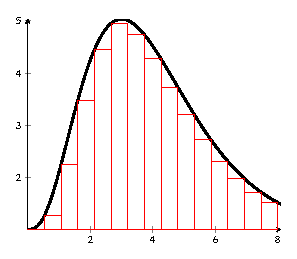
\includegraphics[scale=1,page=1]{lu}
  \hspace{2cm}
  \includegraphics[scale=1,page=2]{lu}
\end{figure}

\begin{prp}%[定積分基本性質]
  令 $f$, $g$ 在包含 $a$, $b$, $c$ 之區間為可積, $\alpha$, $\beta\in\mathbb{R}$. 則
  \begin{enumerate}\setlength{\itemsep}{0pt}
    \item $\ds\int_a^a f(x)\,\text{d}x = 0$
    \item $\ds\int_a^b f(x)\,\text{d}x = -\int_b^a f(x)\,\text{d}x$
    \item $\ds\int_a^b \big(\alpha\,f(x) + \beta\,g(x)\big)\,\text{d}x = \alpha\int_a^b f(x)\,\text{d}x + \beta\int_a^b g(x)\,\text{d}x$
    \item $\ds\int_a^b f(x)\,\text{d}x + \int_b^c f(x)\,\text{d}x = \int_a^c f(x)\,\text{d}x$
    \item $\ds\int_a^b f(x)\,\text{d}x\leqslant\int_a^b g(x)\,\text{d}x$, 若 $f(x)\leqslant g(x)\;\forall\,x\in[a, b],\;a\leqslant b$
    \item $\ds\left|\,\int_a^b f(x)\,\text{d}x\,\right|\leqslant \int_a^b \left|\,f(x)\,\right|\,\text{d}x, \quad a\leqslant b$ 
    \item $f(x)$ 為奇函數: $\ds\int_{-a}^a f(x)\,\text{d}x = 0$
    \item $f(x)$ 為偶函數: $\ds\int_{-a}^a f(x)\,\text{d}x = 2\int_0^a f(x)\,\text{d}x$
  \end{enumerate}
\end{prp}

\begin{ex}
  \begin{enumerate}\setlength{\itemsep}{0pt}
    \item[]
    \item $\ds\int_{-\sqrt{2}}^{\sqrt{2}} \sqrt{2 - x^2}\,\text{d}x = \pi\quad$(半徑 $\sqrt{2}$ 之半圓面積) 
    \item 定義 $\ds\sgn(x)=\begin{cases} 1 & x > 0 \\ -1 & x < 0\end{cases}$, 則 $\ds\int_{-1}^2 \sgn(x)\,\text{d}x = 2\cdot 1 - 1\cdot 1 = 1$
    \item $\ds\int_{-\pi}^{\pi} \sin(x^7-5x^3)\,\text{d}x = 0\quad$($\sin(x^7-5x^3)$ 為奇函數) 
    \item $\ds\int_{-6}^{6} e^{-x^4}\sin(\sin x)\,\text{d}x = 0\quad$($e^{-x^4}\sin(\sin x)$ 為奇函數) 
    \item $\ds\int_{-4}^{4} \big(e^{x} - e^{-x}\big)\,\text{d}x = 0\quad$($e^{x} - e^{-x}$ 為奇函數) 
    \item $\ds\int_{-2024}^{2024} \big(e^{9x^5-2x^7} - e^{-9x^5 + 2x^7}\big)\,\text{d}x = 0\quad$($e^{9x^5-2x^7} - e^{-9x^5 + 2x^7}$ 為奇函數)  
    \item $\ds\int_{-a}^a |x|\,\text{d}x = 2\int_0^a |x|\,\text{d}x = a^2\quad$($|x|$ 為偶函數; 兩 $a\times a$ 等腰直角三角形面積) 
    \item 定義 $\ds\int_1^x\frac{1}{\tau}\,\text{d}\tau = \ln x$, 則 $\ds\int_{\frac{1}{4}}^3\frac{1}{x}\,\text{d}x = \int_{\frac{1}{4}}^1 \frac{1}{x}\,\text{d}x + \int_1^3 \frac{1}{x}\,\text{d}x = -\int_1^{\frac{1}{4}}\frac{1}{x}\,\text{d}x + \int_1^3\frac{1}{x}\,\text{d}x = \ln 12$
    \item $\ds\int_0^2 \sqrt{4 - x^2}\cdot\sgn(1 - x)\,\text{d}x = \int_0^1\sqrt{4 - x^2}\,\text{d}x - \int_1^2\sqrt{4 - x^2}\,\text{d}x = \Big(\frac{4\pi}{12} + \frac{\sqrt{3}}{2}\Big) - \Big(\frac{4\pi}{6} - \frac{\sqrt{3}}{2}\Big) = \sqrt{3} - \frac{\pi}{3}$ 
    \item $\ds\forall\,n\in\mathbb{N},\;\int_n^{n+1}\floor{x}\,\text{d}x = n$ 
  \end{enumerate}
\end{ex}

\subsection*{以極限定義求定積分}

\begin{fact}
  $\ds\sum_{k = 1}^n k^2 = \frac{n(n + 1)(2n + 1)}{6}$. 
\end{fact}

\begin{prf}
  由 $\ds k(k + 1) = \frac{k(k + 1)(k + 2) - (k - 1)k(k + 1)}{3}$, $\ds\sum_{k = 1}^n k(k + 1) = \frac{n(n+1)(n+2)}{3}$. 又 $\ds k^2 = k(k + 1) - k$, $\ds\sum_{k = 1}^n k^2 = \sum_{k = 1}^n \big(k(k + 1) - k\big) = \frac{n(n + 1)(n + 2)}{3} - \frac{n(n + 1)}{2} = \frac{n(n + 1)(2n + 1)}{6}$.  
\end{prf}

\begin{ex}
  求 $\ds\int_0^1 x^2\,\text{d}x$. 
\end{ex}

\begin{sol}
  建立 $\ds [0,\,1]$ 分割 $\ds\mathbb{P}: \Big\{0, \frac{1}{n}, \frac{2}{n}, \ldots, \frac{n}{n}\Big\}$, 則 $\ds\Delta x_k = \frac{1}{n}\;\forall\,k=1,2,\ldots,n$ 且 $\ds\|P\|\to 0$ 當 $n\to\infty$. $f(x) = x^2$ 且 $f$ 在 $[0,\,1]$ 嚴格遞增, $\ds U(f,\mathbb{P}) = \sum_{k=1}^n u_k\,\Delta x_k = \sum_{k=1}^n\frac{k^2}{n^2}\cdot\frac{1}{n} = \frac{1}{n^3}\sum_{k = 1}^n k^2$, $\ds L(f,\mathbb{P}) = \sum_{k=1}^n l_k\,\Delta x_k = \sum_{k=1}^n\frac{(k - 1)^2}{n^2}\cdot\frac{1}{n} = \frac{1}{n^3}\sum_{k = 1}^{n-1}k^2$, $\ds L(f,\mathbb{P})\leqslant R(f,\mathbb{P})\leqslant U(f, \mathbb{P})$. 由 $\ds\sum_{k = 1}^n k^2 = \frac{n(n + 1)(2n + 1)}{6}$, $\ds\lim_{n\to\infty} U(f,\mathbb{P}) = \lim_{n\to\infty}\frac{1}{n^3}\sum_{k = 1}^n k^2 = \lim_{n\to\infty}\frac{n(n + 1)(2 n + 1)}{6n^3} = \frac{1}{3}$, $\ds\lim_{n\to\infty} L(f,\mathbb{P}) = \lim_{n\to\infty}\frac{1}{n^3}\sum_{k = 1}^{n - 1} k^2 = \lim_{n\to\infty}\frac{(n - 1)n(2 n - 1)}{6n^3} = \frac{1}{3}$, 故由夾擊定理 $\ds\lim_{n\to\infty} R(f,\mathbb{P}) = \frac{1}{3}$. 
\end{sol}

\begin{fact}
  若 $r\in\mathbb{R}$, $\ds\sum_{k = 0}^n r^k = \frac{r^{n+1} - 1}{r - 1}$. 
\end{fact}

\begin{prf}
  令 $\ds s = \sum_{k = 0}^n r^k$, 則 $\ds r\,s = \sum_{k = 1}^{n + 1} r^k$; $\ds r\,s - s = r^{n + 1} - 1\ie s = \frac{r^{n + 1} - 1}{r - 1}$.  
\end{prf}

\begin{ex}
  求 $\ds\int_0^1 e^x\,\text{d}x$. 
\end{ex}

\begin{sol}
  建立 $\ds [0,\,1]$ 分割 $\ds\mathbb{P}: \Big\{0, \frac{1}{n}, \frac{2}{n}, \ldots, \frac{n}{n}\Big\}$, 則 $\ds\Delta x_k = \frac{1}{n}\;\forall\,k=1,2,\ldots,n$ 且 $\ds\|P\|\to 0$ 當 $n\to\infty$. $f(x) = e^x$ 且 $f$ 在 $[0,\,1]$ 嚴格遞增, $\ds U(f,\mathbb{P}) = \sum_{k=1}^n u_k\,\Delta x_k = \sum_{k=1}^n e^{\frac{k}{n}}\cdot\frac{1}{n} = \frac{1}{n}\frac{e^{\frac{1}{n}}\big(e^{\frac{n}{n}} - 1\big)}{e^{\frac{1}{n}} - 1} = \frac{e - 1}{n}\frac{e^{\frac{1}{n}}}{e^{\frac{1}{n}} - 1}$, $\ds L(f,\mathbb{P}) = \sum_{k=1}^n l_k\,\Delta x_k = \sum_{k=1}^n e^{\frac{k - 1}{n}}\cdot\frac{1}{n} = \frac{1}{n}\frac{e^0\big(e^{\frac{n}{n}} - 1\big)}{e^{\frac{1}{n}} - 1} = \frac{e - 1}{n}\frac{1}{e^{\frac{1}{n}} - 1}$, $\ds L(f,\mathbb{P})\leqslant R(f,\mathbb{P})\leqslant U(f, \mathbb{P})$. $\ds\lim_{n\to\infty} U(f,\mathbb{P}) = \lim_{n\to\infty}\frac{e - 1}{n}\frac{e^{\frac{1}{n}}}{e^{\frac{1}{n}} - 1} = (e - 1)\lim_{x\to 0+}\frac{x e^x}{e^x - 1} = (e - 1)\lim_{x\to 0+}\frac{e^x + x e^x}{e^x} = e - 1$, $\ds\lim_{n\to\infty} L(f,\mathbb{P}) = \lim_{n\to\infty}\frac{e - 1}{n}\frac{1}{e^{\frac{1}{n}} - 1} = (e - 1)\lim_{x\to 0+}\frac{x}{e^x - 1} = (e - 1)\lim_{x\to 0+}\frac{1}{e^x} = e - 1$, 故由夾擊定理 $\ds\lim_{n\to\infty} R(f,\mathbb{P}) = e - 1$. 
\end{sol}

\begin{fact}
  $\ds\sum_{k = 1}^n \cos kx = \frac{1}{2}\bigg(\frac{\sin\big(n+\frac{1}{2}\big)x}{\sin\frac{x}{2}}-1\bigg)$
\end{fact}

\begin{prf}
  考慮 $\ds\sum_{k = 1}^{n} e^{ikx} = \frac{e^{ix}(1 - e^{inx})}{1 - e^{ix}}$, 則 $\ds\sum_{k = 1}^{n} \cos kx = \Re\Big\{\sum_{k = 1}^n e^{ikx}\Big\} = \Re\Big\{\frac{e^{ix}(1 - e^{inx})}{1 - e^{ix}}\Big\} = \Re\bigg\{\frac{e^{ix}\,e^{\frac{inx}{2}}\big(e^{-\frac{inx}{2}} - e^{\frac{inx}{2}}\big)}{e^{\frac{ix}{2}}\big(e^{-\frac{ix}{2}} - e^{\frac{ix}{2}}\big)}\bigg\} = \frac{\cos\frac{(n+1)x}{2}\,\sin\frac{nx}{2}}{\sin\frac{x}{2}} = \frac{\sin\big(\frac{nx}{2} + \frac{(n + 1)x}{2}\big) + \sin\big(\frac{nx}{2} + \frac{(n + 1)x}{2}\big)}{2\,\sin\frac{x}{2}} = \frac{\sin\big(n+\frac{1}{2}\big)x - \sin\frac{x}{2}}{2\,\sin\frac{x}{2}} = \frac{1}{2}\bigg(\frac{\sin\big(n+\frac{1}{2}\big)x}{\sin\frac{x}{2}}-1\bigg)$.  
\end{prf}

\begin{ex}
  求 $\ds\int_0^{\frac{\pi}{2}}\cos x\,\text{d}x$. 
\end{ex}

\begin{sol}
  建立 $\ds \big[0,\,\frac{\pi}{2}\big]$ 分割 $\ds\mathbb{P}: \Big\{0, \frac{\pi}{2n}, \frac{2\pi}{2n}, \ldots, \frac{n\pi}{2n}\Big\}$, 則 $\ds\Delta x_k = \frac{\pi}{2n}\;\forall\,k=1,2,\ldots,n$ 且 $\ds\|P\|\to 0$ 當 $n\to\infty$, 則積分為 $\ds\lim_{n\to\infty} R(f,\mathbb{P}) = \sum_{k=1}^n f(\xi_k)\,\Delta x_k = \lim_{n\to\infty}\sum_{k=1}^n\cos\frac{k\pi}{2n}\cdot\frac{\pi}{2n}  = \lim_{n\to\infty}\sum_{k=1}^n\cos\Big(k\,\big(\frac{\pi}{2n}\big)\Big)\cdot\frac{\pi}{2n} = \\ \lim_{n\to\infty}\frac{1}{2}\bigg(\frac{\sin\big(\big(n+\frac{1}{2}\big)\cdot\frac{\pi}{2n}\big)}{\sin\big(\frac{1}{2}\cdot\frac{\pi}{2n}\big)}-1\bigg)\cdot\frac{\pi}{2n} = \lim_{n\to\infty}\frac{\sin\big(\big(n+\frac{1}{2}\big)\frac{\pi}{2n}\big)\frac{1}{2}\cdot\frac{\pi}{2n}}{\sin\big(\frac{1}{2}\cdot\frac{\pi}{2n}\big)} = \lim_{n\to\infty}\sin\Big(\frac{1}{2} + \frac{1}{4n}\Big)\pi\cdot\lim_{n\to\infty}\frac{\frac{1}{2}\cdot\frac{\pi}{2n}}{\sin\big(\frac{1}{2}\cdot\frac{\pi}{2n}\big)} = \sin\frac{\pi}{2}\cdot 1 = 1$.
\end{sol}

\subsection*{微積分基本定理}

\begin{thm}[微積分基本定理 (Fundamental Theorem of Calculus, FTC) ]
  \begin{enumerate}\setlength{\itemsep}{0pt}
    \item[]
    \item 若 $f$ 在 $[a,\,b]$ 連續, 令 $\ds F(x) = \int_a^x f(\tau)\,\text{d}\tau$ 且 $a\leqslant x\leqslant b$, 則 $\ds F'(x) = f(x)\;\forall\,x\in[a,\,b]$. 
    \item 若 $\ds G'(x) = f(x)\;\forall\,x\in[a,\,b]$, 則 $\ds\int_a^b f(x)\,\text{d}x = G(b) - G(a) \equiv G(x)\,\Big|_a^b$. 
  \end{enumerate}
\end{thm}
\begin{rmk}
  由 FTC, $\ds\int_a^b f(x)\,\text{d}x$ 可由 $f$ 的反導函數 (不定積分) 得出, 不需繁複極限計算!
\end{rmk}

\begin{prf}
  \begin{enumerate}\setlength{\itemsep}{0pt}
    \item[]
    \item WLOG 令 $h > 0$. 則 $\ds\Bigg|\,\frac{F(x + h) - F(x)}{h} - f(x)\,\Bigg| = \Bigg|\,\frac{1}{h}\int_x^{x + h}(f(\tau) - f(x))\,\text{d}\tau\,\Bigg| \leqslant\frac{1}{h}\int_x^{x + h}\big|\,f(\tau) - f(x)\big|\,\text{d}\tau \leqslant\max_{x\leqslant\tau\leqslant x+h}\big|\,f(\tau) - f(x)\big|\to 0$, 當 $h\to 0$ 且 $f$ 為連續. 
    \item $\ds(G(x) - F(x))' = f(x) - f(x) = 0\;\forall\,x\in[a, b]$, 故 $\ds G(x) - F(x)$ 在 $[a, b]$ 為常數 $\ds\ie G(a) - F(a) = G(b) - F(b) \ie G(b) - G(a) = F(b) - F(a) = \int_a^b f(x)\,\text{d}x$. 
  \end{enumerate}
\end{prf}

\begin{ex}[以 FTC 求定積分]
  \begin{enumerate}\setlength{\itemsep}{0pt}
    \item[]
    \item $\ds x^2$ 之反導函數為 $\ds\frac{x^3}{3}$, 故 $\ds\int_0^1 x^2\,\text{d}x = \frac{1^3}{3} - \frac{0^3}{3} = \frac{1}{3}$. 
    \item $\ds e^x$ 之反導函數為 $\ds e^x$, 故 $\ds\int_0^1 e^x\,\text{d}x = e^1 - e^0 = e - 1$. 
    \item $\cos x$ 之反導函數為 $\sin x$, 故 $\ds\int_0^{\frac{\pi}{2}}\cos x\,\text{d}x = \sin\frac{\pi}{2} - \sin 0 = 1$. 
  \end{enumerate}
\end{ex}

\begin{fact}[定積分變數變換]
  \begin{itemize}\setlength{\itemsep}{0pt}
    \item[]
    \item 求反導函數後代入: $\ds\int_a^b f'(g(x))\,g'(x)\,\text{d}x = f(g(x))\,\Big|_{x = a}^{x = b} = f(g(b)) - f(g(a))$
    \item 變數變換並改變積分範圍: $\ds\int_a^b f'(g(x))\,g'(x)\,\text{d}x = \int_a^b f'(g(x))\,\text{d}g(x) =\int_{g(a)}^{g(b)} f'(u)\,\text{d}u = f(u)\,\Big|_{u = g(a)}^{u = g(b)} = f(g(b)) - f(g(a))$
  \end{itemize}
\end{fact}

\begin{ex}
  求 $\ds\int_0^1 x^3(1 + x^4)^3\,\text{d}x$. 
\end{ex}

\begin{sol}
  \begin{itemize}\setlength{\itemsep}{0pt}
    \item[]
    \item 求反導函數後代入: 令 $\ds u = 1 + x^4$, 則 $\ds\text{d}u = 4 x^3\,\text{d}x\ie x^3\,\text{d}x = \frac{\text{d}u}{4}$, 故 $\ds\int x^3(1 + x^4)^3\,\text{d}x = \int (1 + x^4)^3\,x^3\,\text{d}x = \int u^3\,\frac{\text{d}u}{4} = \frac{u^4}{16} + c = \frac{(1 + x^4)^4}{16} + c$. 故 $\ds\int_0^1 x^3(1 + x^4)^3\,\text{d}x = \frac{(1 + x^4)^4}{16}\,\Big|_{x = 0}^{x = 1} = \frac{(1 + 1^4)^4 - (1 + 0^4)^4}{16} = \frac{15}{16}$. 
    \item 變數變換並改變積分範圍: 令 $\ds u = 1 + x^4$, 則 $\ds\text{d}u = 4 x^3\,\text{d}x\ie x^3\,\text{d}x = \frac{\text{d}u}{4}$. 積分範圍 $x$ 由 $0$ 至 $1$, 則變數變換後 $u$ 由 $\ds 1 + 0^4 = 1$ 至 $\ds1 + 1^4 = 2$, 故 $\ds\int_0^1 x^3(1 + x^4)^3\,\text{d}x = \int_0^1 (1 + x^4)^3\,x^3\,\text{d}x = \int_1^2 u^3\,\frac{\text{d}u}{4} = \frac{1}{4}\int_1^2 u^3\,\text{d}u = \frac{1}{16} u^4\,\Big|_{u = 1}^{u = 2} = \frac{2^4 - 1^4}{16} = \frac{15}{16}$. 
  \end{itemize}
\end{sol}

\begin{ex}
  求 $\ds\int_0^{\sqrt{3}}\!\frac{4x}{\sqrt{1 + x^2}}\,\text{d}x$. 
\end{ex}

\begin{sol}
  \begin{itemize}\setlength{\itemsep}{0pt}
    \item[]
    \item 求反導函數後代入: 令 $\ds u = 1 + x^2$, 則 $\ds\text{d}u = 2 x\,\text{d}x\ie 4x\,\text{d}x = 2\,\text{d}u$, 故 $\ds\int\!\frac{4x}{\sqrt{1 + x^2}}\,\text{d}x = \int\!\frac{2}{\sqrt{u}}\,\text{d}u = 4\sqrt{u} + c = 4\sqrt{1 + x^2} + c$. 故 $\ds\int_0^{\sqrt{3}}\frac{4x}{\sqrt{1 + x^2}}\,\text{d}x = 4\sqrt{1 + x^2}\,\Big|_{x = 0}^{x = \sqrt{3}} = 4\sqrt{1 + 3} - 4\sqrt{1} = 4$. 
    \item 變數變換並改變積分範圍: 令 $\ds u = 1 + x^2$, 則 $\ds\text{d}u = 2 x\,\text{d}x\ie 4x\,\text{d}x = 2\,\text{d}u$. 積分範圍 $x$ 由 $0$ 至 $\sqrt{3}$, 則變數變換後 $u$ 由 $\ds1 + 0^2 = 1$ 至 $\ds1 + (\sqrt{3})^2 = 4$, 故 $\ds\int_0^{\sqrt{3}}\frac{4x}{\sqrt{1 + x^2}}\,\text{d}x = \int_1^4 \frac{2}{\sqrt{u}}\,\text{d}u = 4\sqrt{u}\,\Big|_{u = 1}^{u = 4} = 4\,(\sqrt{4} - \sqrt{1}) = 4$. 
  \end{itemize}
\end{sol}

\begin{ex}
  求 $\ds\int_0^{\pi}3\cos^2 x\sin x\,\text{d}x$. 
\end{ex}

\begin{sol}
  \begin{itemize}\setlength{\itemsep}{0pt}
    \item[]
    \item 求反導函數後代入: 令 $\ds u = \cos x$, 則 $\ds\text{d}u = -\sin x\,\text{d}x\ie \sin x\,\text{d}x = -\text{d}u$, 故 $\ds\int3\cos^2 x\sin x\,\text{d}x = -3\int u^2\,\text{d}u = -u^3 + c = -\cos^3 x + c$. 故 $\ds\int_0^{\pi}3\cos^2 x\sin x\,\text{d}x = -\cos^3 x\,\Big|_{x = 0}^{x = \pi} = -(\cos^3\pi - \cos^3 0) = -((-1)^3 - 1^3) = 2$. 
    \item 變數變換並改變積分範圍: 令 $\ds u = \cos x$, 則 $\ds\text{d}u = -\sin x\,\text{d}x\ie \sin x\,\text{d}x = -\text{d}u$. 積分範圍 $x$ 由 $0$ 至 $\pi$, 則變數變換後 $u$ 由 $\ds\cos 0 = 1$ 至 $\ds\cos\pi= -1$, 故 $\ds\int_0^{\pi}3\cos^2 x\sin x\,\text{d}x = -\int_{1}^{-1}3u^2\,\text{d}u = -u^3\,\Big|_{u = 1}^{u = -1} = -((-1)^3 - 1^3) = 2$. 
  \end{itemize}
\end{sol}

\begin{ex}
  若 $f$ 在 $[a, b]$ 二次可微且 $f(a) = f(b) = 0$, 證明 $\ds\int_a^b\!(x-a)(b-x)\,f''(x)\,\text{d}x = -2\int_a^b\!f(x)\,\text{d}x$.
\end{ex}

\begin{sol}
  $\ds\int_a^b\!(x-a)(b-x)\,f''(x)\,\text{d}x = \big((x - a)(b - x)\,f'(x) - (a + b - 2 x)\,f(x)\big)\,\Big|_a^b - 2\int_a^b f(x)\,\text{d}x = \big((b - a)(b - b)\,f'(b) - (a + b - 2 b)\,f(b)\big) - \big((a - a)(b - a)\,f'(a) - (a + b - 2 a)\,f(a)\big) - 2\int_a^b f(x)\,\text{d}x = -2\int_a^b f(x)\,\text{d}x$. 

  \begin{minipage}{0.35\textwidth}
    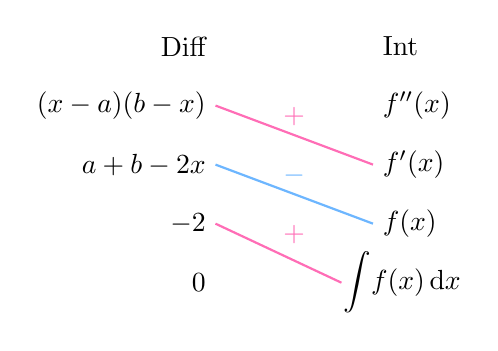
\begin{tikzpicture}[yscale=0.75]
      \draw (-1, 1) node[left]{Diff};
      \draw (1,  1) node[right]{Int};
      \draw (-1, -0) node[left]{$(x - a)(b - x)$};
      \draw (1,  -0) node[right]{$f''(x)$};
      \draw (-1, -1) node[left]{$a + b - 2x$};
      \draw (-1, -2) node[left]{$-2$};
      \draw (-1, -3) node[left]{$0$};
      \draw (1,  -1) node[right]{$f'(x)$};
      \draw (1,  -2) node[right]{$f(x)$};
      \draw (0.5,  -3) node[right]{$\ds\int\!f(x)\,\text{d}x$};
      \draw[thick, M4, -] (-1, -0)--(1, -1); \draw[M4] (0, -0.5) node[above]{$+$};
      \draw[thick, C4, -] (-1, -1)--(1, -2); \draw[C4] (0, -1.5) node[above]{$-$};
      \draw[thick, M4, -] (-1, -2)--(0.6, -3); \draw[M4] (0, -2.5) node[above]{$+$};
    \end{tikzpicture}
  \end{minipage}
  \hspace{5mm}
  \begin{minipage}{0.65\textwidth}
    $\ds\int(x-a)(b-x)\,f''(x)\,\text{d}x \\= \big((x - a)(b - x)\,f'(x) - (a + b - 2 x)\,f(x)\big) - 2\int\!f(x)\,\text{d}x$
  \end{minipage}
\end{sol}

\begin{prp}
  令 $\ds F(x) = \int_{v(x)}^{u(x)}\!f(\tau)\,\text{d}\tau$, 則 $\ds F'(x) = f(u(x))\cdot u'(x) - f(v(x))\cdot v'(x)$. 
\end{prp}

\begin{prf}
  令 $a\in\mathbb{R}$, $\ds F(x) = \int_{v(x)}^{u(x)}\!f(\tau)\,\text{d}\tau = \int_{a}^{u(x)}\!f(\tau)\,\text{d}\tau - \int_{a}^{v(x)}\!f(\tau)\,\text{d}\tau$. 令 $\ds G(x)\equiv\int_a^x f(\tau)\,\text{d}\tau$, 則 $\ds G'(x) = f(x)$, $\ds F(x) = \int_{a}^{u(x)} f(\tau)\,\text{d}\tau - \int_{a}^{v(x)} f(\tau)\,\text{d}\tau = G(u(x)) - G(v(x))$; 故 $\ds F'(x) = (G(u(x)) - G(v(x)))' = G'(u(x))\cdot u'(x) - G'(v(x))\cdot v'(x) = f(u(x))\cdot u'(x) - f(v(x))\cdot v'(x)$.   
\end{prf}

\begin{ex} 
  \begin{enumerate}\setlength{\itemsep}{0pt}
    \item[]
    \item $\ds F(x) = \int_1^x\!\frac{1}{1 + \tau^4}\,\text{d}\tau \ie F'(x) = \frac{1}{1 + x^4}$ 
    \item $\ds F(x) = \int_2^{\sqrt{x}}\!\sin\tau\,\text{d}\tau \ie F'(x) = \sin\sqrt{x}\cdot\frac{1}{2\sqrt{x}}$
    \item $\ds F(x) = \int_{x}^{2x}\!\tau^3\,\text{d}\tau \ie F'(x) = (2x)^3\cdot 2 - x^3\cdot 1 = 15x^3$
    \item $\ds F(x) = \int_{\sin x}^{\tan^{-1}x}\!e^{\tau^2}\,\text{d}\tau \ie F'(x) = e^{(\tan^{-1}x)^2}\cdot\frac{1}{1 + x^2} - e^{\sin^2 x}\cdot\cos x$
  \end{enumerate}
\end{ex}

\begin{ex}
  若 $\ds g(x) = \int_0^{\cos x}\!(1 + \sin(t^2))\,\text{d}t$, $\ds f(x) = \int_0^{g(x)}\!\!\frac{1}{\sqrt{1 + t^3}}\,\text{d}t$, 求 $\ds f'\Big(\frac{\pi}{2}\Big)$. 
\end{ex}

\begin{sol}
  $\ds f'(x) = \frac{1}{\sqrt{1 + g(x)^3}}\cdot g'(x)$, $\ds g'(x) = (1 + \sin(\cos^2 x))\cdot(-\sin x)$. 代入 $\ds x=\frac{\pi}{2}$, $\ds g\Big(\frac{\pi}{2}\Big) = 0$, $\ds g'\Big(\frac{\pi}{2}\Big) = -1$, 故 $\ds f'\Big(\frac{\pi}{2}\Big) = -1$.  
\end{sol}

\begin{ex}
  若 $\ds\int_0^{x^2}\!\! f(t)\,\text{d}t = x\sin\pi x$, 求 $f'(9)$. 
\end{ex}

\begin{sol}
  $\ds\int_0^{x^2}\!\! f(t)\,\text{d}t = x\sin\pi x$ 兩邊對 $x$ 微分得 $\ds f(x^2)\cdot 2x = \sin\pi x + x\cdot\pi\cos\pi x$. 兩邊再對 $x$ 微分得 $\ds (f'(x^2)\cdot 2x)\cdot 2x + f(x^2)\cdot 2 = \pi\cos\pi x + \pi\cos\pi x - x\cdot\pi^2\sin\pi x$. 代入 $x = 3$, 則 $\ds (f'(9)\cdot 2\cdot 3)\cdot 2\cdot 3 + f(9)\cdot 2 = \pi\cos3\pi + \pi\cos3\pi - 3\cdot\pi^2\sin3\pi \ie f'(9)\cdot 36 + f(9)\cdot 2 = -2\pi$. 又 $\ds f(3^2)\cdot(2\cdot 3) = \sin 3\pi + 3\cdot\pi\cos3\pi\ie f(9) = -\frac{\pi}{2}$, 故 $\ds f'(9) = -\frac{\pi}{36}$.  
\end{sol}

\begin{ex}
  求函數 $f$ 與 $a\in\mathbb{R}$ 使 $\ds 6 + \int_a^x\frac{f(t)}{t^2}\,\text{d}t = 2\sqrt{x}$, $\forall\,x > 0$.  
\end{ex}

\begin{sol}
  $\ds 6 + \int_a^x\frac{f(t)}{t^2}\,\text{d}t = 2\sqrt{x}$ 兩邊對 $x$ 微分得 $\ds\frac{f(x)}{x^2} = \frac{1}{\sqrt{x}}\ie f(x) = x^{\frac{3}{2}}$. 代入原式得 $\ds 6 + \int_a^x\frac{t^{\frac{3}{2}}}{t^2}\,\text{d}t = 6 + \int_a^x\!\frac{1}{\sqrt{t}}\,\text{d}t = 6 + 2\sqrt{t}\,\Big|_a^x = 6 + 2\sqrt{x} - 2\sqrt{a} = 2\sqrt{x} \ie a = 9$. 
\end{sol}

\begin{ex}
  求下列極限. 
  \setlength{\columnsep}{-35mm}
  \begin{multicols}{2}
    \begin{enumerate}\setlength{\itemsep}{0pt}
      \item $\ds\lim_{x\to 0}\frac{\int_0^x(\sec t - 1)\,\text{d}t}{x^3}$
      \item $\ds\lim_{x\to\infty}\frac{\int_{x^2}^0 e^{t - x^2}(2 t^2 + 1)\,\text{d}t}{x^4}$
      \item $\ds\lim_{x\to 0}\frac{1}{x}\int_0^{\tan x}\!\!f(u)(\sin x - \cos u)\,\text{d}u$, $f$ 為連續函數
    \end{enumerate}
  \end{multicols}
\end{ex}

\begin{sol}
  \begin{enumerate}\setlength{\itemsep}{0pt}
    \item[]
    \item $\ds\lim_{x\to 0}\frac{\int_0^x(\sec t - 1)\,\text{d}t}{x^3} = \lim_{x\to 0}\frac{\sec x - 1}{3x^2} = \lim_{x\to 0}\frac{\sec x\tan x}{6x} = \lim_{x\to 0}\frac{\sec x\tan x\cdot\tan x + \sec x\cdot\sec^2 x}{6} = \frac{1}{6}$. 
    \item $\ds\lim_{x\to\infty}\frac{\int_{x^2}^0 e^{t - x^2}(2 t^2 + 1)\,\text{d}t}{x^4} = \lim_{x\to\infty}\frac{\int_{x^2}^0 e^t(2 t^2 + 1)\,\text{d}t}{e^{x^2}x^4} = \lim_{x\to\infty}\frac{-e^{x^2}(2(x^2)^2 + 1)\cdot 2x}{e^{x^2}\,2x\cdot x^4 + e^{x^2}\cdot 4x^3} = \lim_{x\to\infty}\frac{-(4x^5 + 2x)}{2x^5 + 4x^3} = -2$. 
    \item $\ds\lim_{x\to 0}\frac{1}{x}\int_0^{\tan x}\!\!f(u)(\sin x - \cos u)\,\text{d}u = \lim_{x\to 0}\frac{\int_0^{\tan x}\!f(u)(\sin x - \cos u)\,\text{d}u}{x} \\= \lim_{x\to 0}\frac{\sin x\int_0^{\tan x}\!f(u)\,\text{d}u - \int_0^{\tan x}\!f(u)\cos u\,\text{d}u}{x} \\ = \lim_{x\to 0}\frac{\cos x\int_0^{\tan x}\!f(u)\,\text{d}u + \sin x\cdot f(\tan x)\cdot\sec^2 x - f(\tan x)\cos(\tan x)\cdot\sec^2 x}{1} = -f(0)$
  \end{enumerate}
\end{sol}

\section*{4.3 面積與體積}
\subsection*{面積}
\begin{fact}
  \begin{minipage}{\textwidth}
    當 $f(x)\geqslant 0$ $\forall\,x\in [a,\,b]$, $\ds\int_a^b\!f(x)\,\text{d}x$ 為 $y = f(x)$, $x$ 軸, $x = a$, 與 $x = b$ 所圍成之面積. 
  \end{minipage}
  \begin{minipage}{\textwidth}
    \begin{center}
      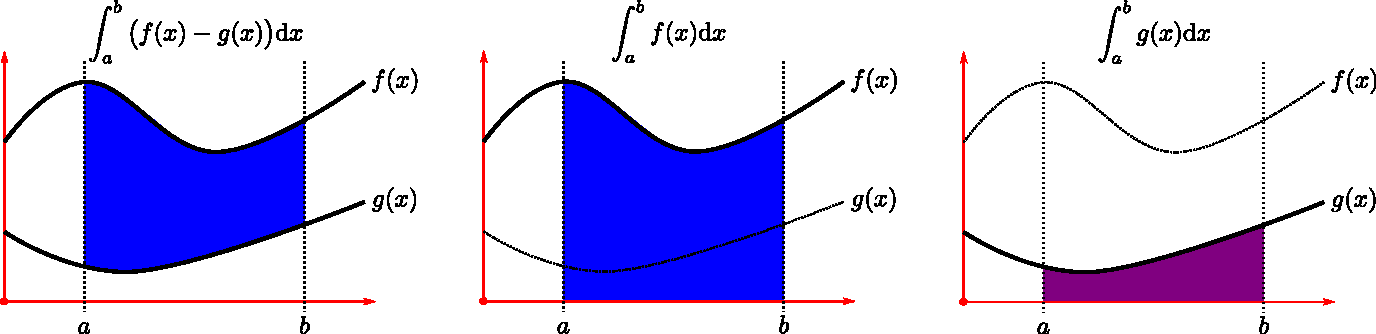
\includegraphics[width=.9\textwidth]{area_between2}
    \end{center}
  \end{minipage}
  \begin{minipage}{.42\textwidth}
    \begin{center}
      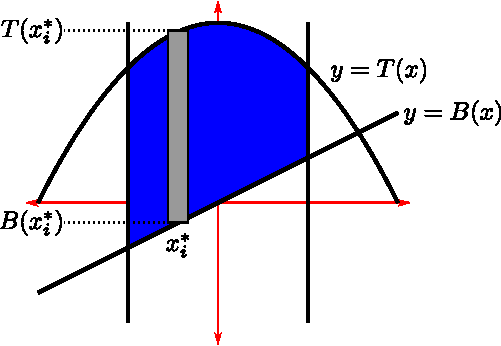
\includegraphics[scale=.7]{area_between4}
    \end{center}
  \end{minipage}
  \begin{minipage}{.58\textwidth}
    \begin{align*}
      &\text{(面積)} \,\approx\,\sum_{i=1}^n\big(T(x_i^*) - B(x_i^*)\big)\,\Delta x,\;\Delta x = \frac{b - a}{n} \\
      &\lim_{n\to\infty}\sum_{i=1}^n \big(T(x_i^*)- B(x_i^*)\big)\,\Delta x = \int_a^b \big(T(x) - B(x)\big)\,\text{d}x
    \end{align*}
  \end{minipage}
\end{fact}

\begin{ex}           
  求以 $y = 4 - x^2$, $y = x$, $x = -1$, 與 $x=1$ 圍成之區域面積.
\end{ex}

\begin{sol}
  \begin{minipage}{.4\textwidth}
    \hspace{1cm}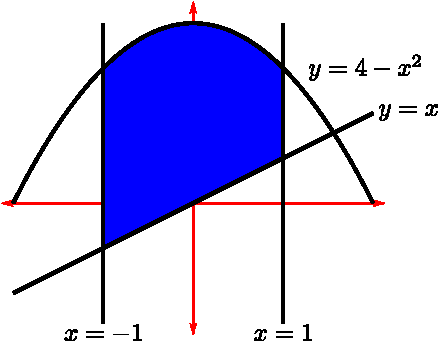
\includegraphics[scale=.7]{area_between3}
  \end{minipage}
  \begin{minipage}{.6\textwidth}
    \begin{align*}
      \text{(面積)} = \int_{-1}^1\!\big((4 - x^2) - x\big)\,\text{d}x = \frac{22}{3}
    \end{align*}
  \end{minipage}
\end{sol}

\begin{ex}
  求 $y = x^2$ 與 $y = 6x - 2x^2$ 圍成之區域面積.
\end{ex}

\begin{sol}
  \begin{minipage}{.3\textwidth}
    \hspace{5mm}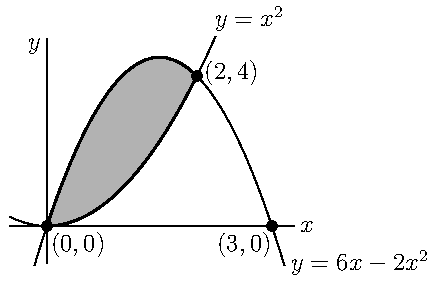
\includegraphics[scale=1]{areaSMPL}
  \end{minipage}
  \begin{minipage}{.7\textwidth}
    \begin{align*}
      \text{(面積)} = \int_0^2\!\big((6x - 2x^2) - x^2\big)\,\text{d}x = 4
    \end{align*}
  \end{minipage}
\end{sol}

\begin{ex}
  求 $\ds y = \frac{1}{\sqrt{2}}$ 與 $y = \sin x$ 在 $x$ 從 $0$ 至 $\ds\frac{\pi}{2}$ 範圍內圍成之區域面積.
\end{ex}

\begin{sol}
  \begin{minipage}{.3\textwidth}
    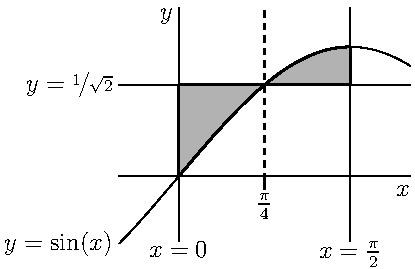
\includegraphics[scale=1]{areaCross} 
  \end{minipage}
  \begin{minipage}{.7\textwidth}
    \begin{align*}
      \text{(面積)} = \int_0^{\frac{\pi}{4}}\!\Big(\frac{1}{\sqrt{2}} - \sin x\Big)\,\text{d}x + \int_{\frac{\pi}{4}}^{\frac{\pi}{2}}\!\Big(\sin x - \frac{1}{\sqrt{2}}\Big)\,\text{d}x = \sqrt{2} - 1
    \end{align*}
  \end{minipage}
\end{sol}

\begin{ex}
  \begin{minipage}{.5\textwidth}
    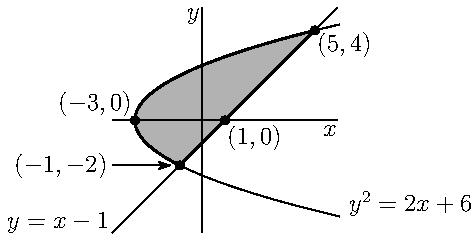
\includegraphics[scale=1]{areaY}
  \end{minipage}
  \begin{minipage}{.5\textwidth}
    求 $y^2 = 2x + 6$ 與 $y = x - 1$ 圍成之區域面積.
  \end{minipage}
\end{ex}

\begin{sol}
  \begin{minipage}{.48\textwidth}
    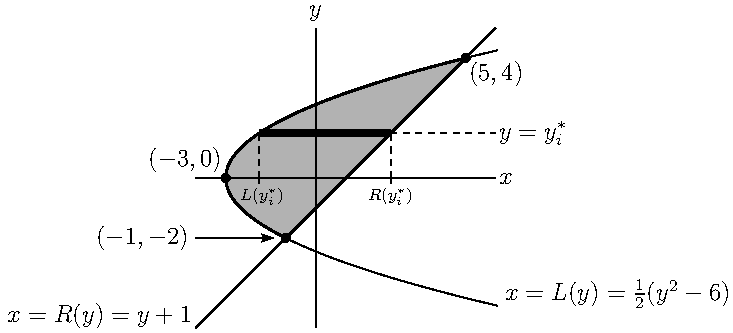
\includegraphics[scale=.8]{areaYhor}
  \end{minipage}
  \begin{minipage}{.52\textwidth}
    \begin{align*}
      \text{(面積)} = \int_{-2}^4\!\Big((y + 1) - \frac{1}{2}\,\big(y^2 - 6\big)\Big)\,\text{d}y = 18
    \end{align*}
  \end{minipage}
  \qquad
  \begin{minipage}{.4\textwidth}
    \hspace{3mm}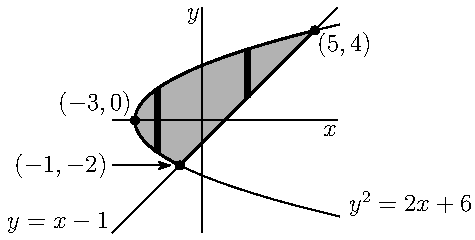
\includegraphics[scale=1]{areaYvert}
  \end{minipage}
  \begin{minipage}{.6\textwidth}
    \begin{align*}
      \text{(面積)} = \int_{-3}^{-1}\!2\sqrt{2x + 6}\,\text{d}x + \int_{-1}^5\!\big(\sqrt{2x + 6} - x + 1\big)\,\text{d}x = 18
    \end{align*}
  \end{minipage}
\end{sol}

\begin{ex}
  求高 $h$ 與底半徑 $r$ 之圓錐體體積. 
\end{ex}

\begin{sol}
  \begin{minipage}{.6\textwidth}
    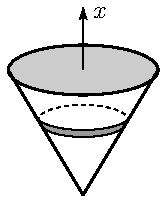
\includegraphics[scale=1.3]{cone}\;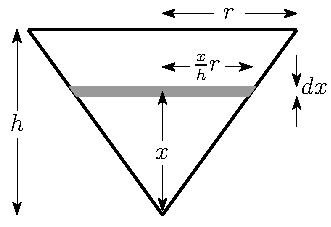
\includegraphics[scale=.9]{coneX}\;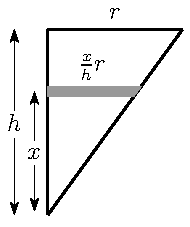
\includegraphics[scale=.9]{coneT}
  \end{minipage}
  \begin{minipage}{.35\textwidth}
    \begin{align*}
      \text{(體積)} = \int_0^h\!\pi\,\Big(\frac{x}{h}\,r\Big)^2\,\text{d}x = \frac{1}{3}\pi r^2 h
    \end{align*}
  \end{minipage}
\end{sol}

%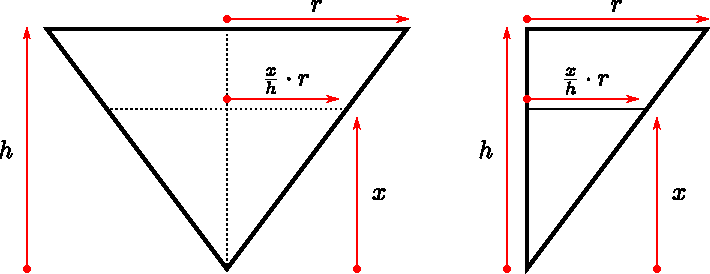
\includegraphics[width=0.7\textwidth]{cone_adr1}
%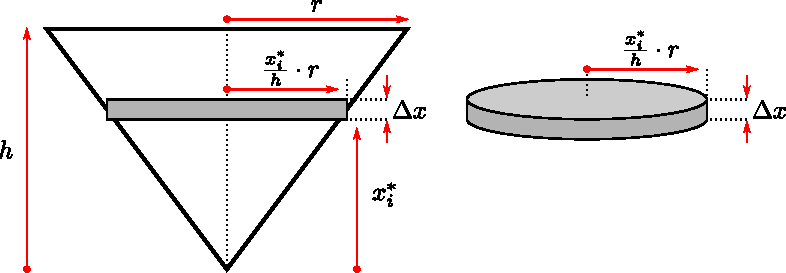
\includegraphics[width=0.85\textwidth]{cone_adr2}

\begin{ex}
  求半徑 $r$ 之三維球體體積.
\end{ex}

\begin{sol}
  \begin{minipage}{.3\textwidth}
    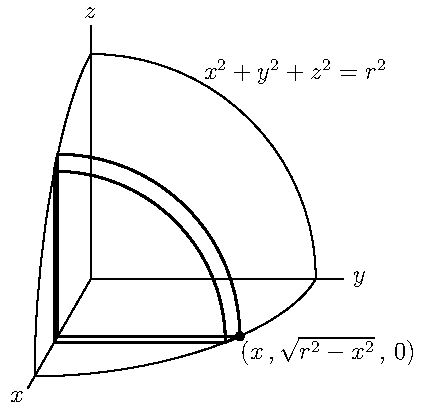
\includegraphics[scale=.7]{sphereSlice} 
  \end{minipage}
  \begin{minipage}{.65\textwidth}
    \begin{align*}
      \text{(體積)} = 8\cdot\int_0^r\!\frac{\pi}{4}\,\big(\sqrt{r^2 - x^2}\big)^2\,\text{d}x = \frac{4}{3}\pi r^3
    \end{align*}
  \end{minipage}
\end{sol}

\begin{ex}
  求以 $y = 3$, $y = 5$, $x = 0$ 與 $x = 4$ 圍成之區域繞 $y = 2$ 旋轉而成之旋轉體體積.
\end{ex}

\begin{sol}
  \begin{minipage}{.6\textwidth}
    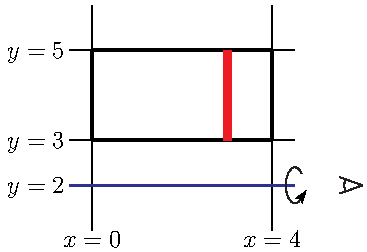
\includegraphics[scale=1]{revolveA} 
    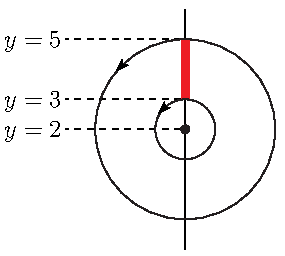
\includegraphics[scale=1]{revolveB} 
  \end{minipage}
  \begin{minipage}{.35\textwidth}
    \begin{align*}
      \text{(體積)} = \int_0^4\!\pi(3^2 - 1^2)\,\text{d}x = 32\pi
    \end{align*}
  \end{minipage}
\end{sol}

\begin{ex}
  求以 $y = \sqrt{x}$, $y = 0$, $x = 0$ 與 $x = 4$ 圍成之區域繞 (i) $y = 0$ (ii) $x = 0$ 旋轉而成之旋轉體體積.
\end{ex}

\begin{sol}
  \begin{minipage}{\textwidth}
    \hspace{5mm}
    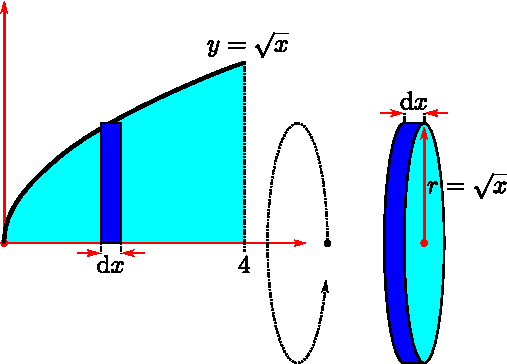
\includegraphics[scale=.8]{rot_rootx1} 
    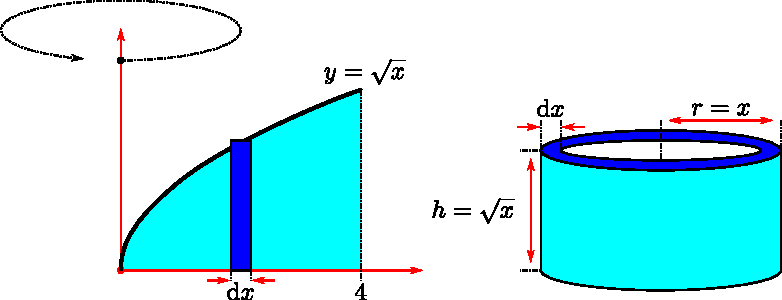
\includegraphics[scale=.8]{rot_rootx2} 
  \end{minipage}
  \begin{minipage}{.5\textwidth}
    \begin{align*}
      \text{(體積)} = \int_0^4\!\pi\,(\sqrt{x})^2\,\text{d}x = 8\pi
    \end{align*}
  \end{minipage}
  \begin{minipage}{.5\textwidth}
    \begin{align*}
      \text{(體積)} = \int_0^4\!2\pi\cdot x\cdot\sqrt{x}\,\text{d}x = \frac{128\pi}{5}
    \end{align*}
  \end{minipage}
  \begin{minipage}{.65\textwidth}
    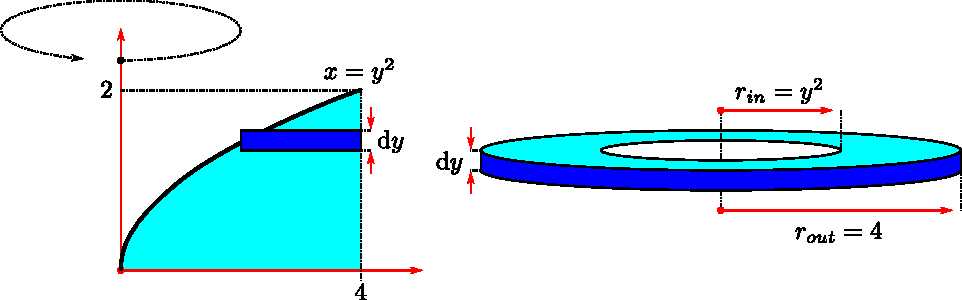
\includegraphics[scale=.75]{rot_rootx3} 
  \end{minipage}
  \begin{minipage}{.35\textwidth}
    \begin{align*}
      \text{(體積)} = \int_0^2\!\pi(4^2 - (y^2)^2)\,\text{d}y = \frac{128\pi}{5}
    \end{align*}
  \end{minipage}
\end{sol}

\begin{ex}
  求高為 $h$, 底面為邊長 $b$ 正方形之錐體體積. 
\end{ex}

\begin{sol}
  \begin{minipage}{0.5\textwidth}
    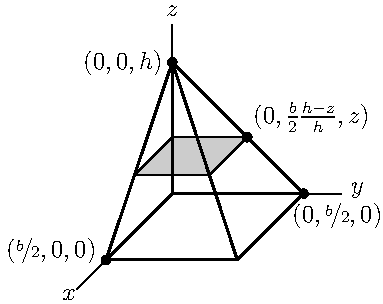
\includegraphics[scale=.8,page=1]{pyramid}
    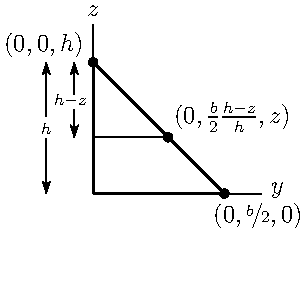
\includegraphics[scale=.8,page=1]{pyramidYZ}
  \end{minipage}
  \begin{minipage}{0.45\textwidth}
    \begin{align*}
      \text{(體積)} = \int_0^h\,\Big(b - \frac{z}{h}\,b\Big)^2\,\text{d}z = \frac{1}{3}\,b^2h
    \end{align*}
  \end{minipage}
\end{sol}

%\begin{ex}
%  Suppose you make two napkin rings by drilling holes with different diameters through two wooden balls. One ball has radius $r$ and the other radius $R$ with $r<R$. You choose the diameter of the holes so that both napkin rings have the same height, $2h$. See the figure below.
%\begin{figure}
%  \centering
%   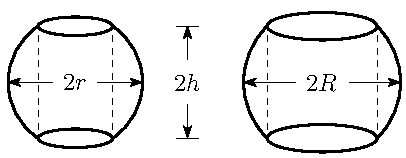
\includegraphics{napkin}
%\end{figure}
%\end{ex}
%
%\begin{sol}
%\begin{itemize}
% \item To compute the volume of the napkin ring of radius $R$, we slice it up into thin horizontal ``pancakes''. Here is a sketch of the part of the napkin ring in the first octant showing a typical pancake.
%\begin{figure}
%  \centering
%   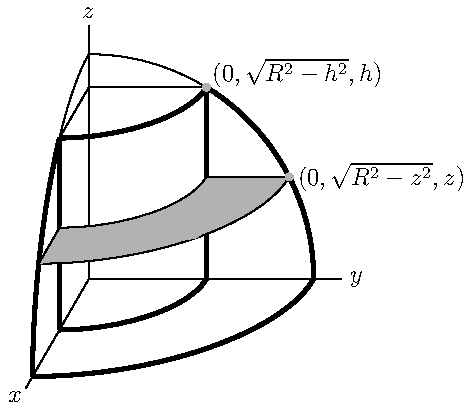
\includegraphics{napkinRing}
%\end{figure}
%\item The coordinates of the two points marked in the $yz$--plane of that figure are found by remembering that
%\begin{itemize}\itemsep1pt \parskip0pt \parsep0pt
%  \item the equation of the sphere is $x^2+y^2+z^2=R^2$.
%  \item The two points have $y>0$ and are in the $yz$--plane, so that $x=0$ for them. So $y=\sqrt{R^2-z^2}$. 
%  \item In particular, at the top of the napkin ring $z=h$, so that $y=\sqrt{R^2-h^2}$.
%\end{itemize}
%\item The pancake at height $z$, shown in the sketch, is a ``washer'' --- a circular disk with a circular hole cut in its center.
%\begin{itemize}
%  \item The outer radius of the washer is $\sqrt{R^2-z^2}$ and
%  \item the inner radius of the washer is $\sqrt{R^2-h^2}$. So the
%\item  cross--sectional area of the washer is
%\begin{align*}
%\pi\big(\sqrt{R^2-z^2}\,\big)^2-\pi\big(\sqrt{R^2-h^2}\,\big)^2
%=\pi(h^2-z^2)
%\end{align*}
%\end{itemize}
%\item The pancake at height $z$
%\begin{itemize}
%\item has thickness $dz$ and
%\item cross--sectional area $\pi(h^2-z^2)$ and hence
%\item volume $\pi(h^2-z^2)\text{d}z$.
%\end{itemize}
%\item Since $z$ runs from $-h$ to $+h$, the total volume
%of wood in the napkin ring of radius $R$ is
%\begin{align*}
%\int_{-h}^h \pi(h^2-z^2)\text{d}z
%&=\pi\Big[h^2z-\frac{z^3}{3}\Big]_{-h}^h \\
%&=\pi\Big[\Big(h^3-\frac{h^3}{3}\Big)
%          -\Big((-h)^3-\frac{(-h)^3}{3}\Big)\Big]\\
%&=\pi\Big[\frac{2}{3}h^3-\frac{2}{3}\big(-h\big)^3\Big] \\
%&=\frac{4\pi}{3}h^3
%\end{align*}
%\end{itemize}
%This volume is independent of $R$. Hence the napkin ring of radius $r$ contains precisely the same volume of wood as the napkin ring of radius $R$!
%\end{sol}

\begin{ex}
  \begin{minipage}{0.15\textwidth}
    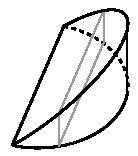
\includegraphics[scale=1,page=1]{notch2}
  \end{minipage}
  \begin{minipage}{0.8\textwidth}
    將一半徑為 $a$ 之圓柱體水平橫切, 再對其底面圓心 $45^\circ$ 角斜切, 求如圖所示結果體積。
  \end{minipage}
\end{ex}

\begin{sol}
  \vspace{3mm}
  \begin{minipage}{0.55\textwidth}
    \begin{center}
      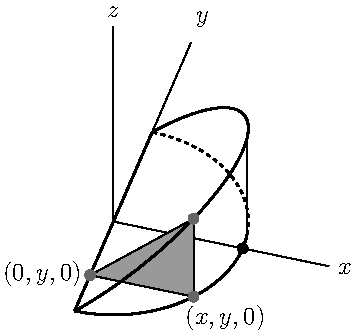
\includegraphics[scale=0.8,page=1]{notch3a}\quad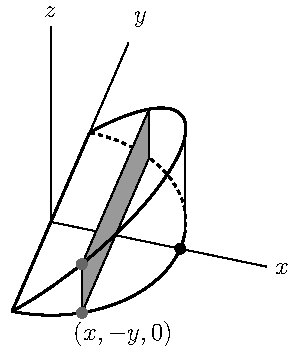
\includegraphics[scale=0.8,page=1]{notch2a}
    \end{center}
  \end{minipage}
  \begin{minipage}{0.4\textwidth}
    \begin{align*}
      \text{(體積)} = \int_{-a}^a\,\frac{1}{2}\,\big(\sqrt{a^2 - y^2}\big)^2\,\text{d}y = \frac{2}{3}\,a^3
    \end{align*}
    \begin{align*}
      \text{(體積)} = \int_0^a x\cdot 2\sqrt{a^2-x^2}\,\text{d}x = \frac{2}{3}\,a^3
    \end{align*}
  \end{minipage}
\end{sol}

\section*{4.4 積分技巧}
\subsection*{部份分式}

\begin{ex}[動機]
  若 $a\ne 0$, 求 $\ds\int\!\!\frac{1}{x^2 - a^2}\,\text{d}x$. 
\end{ex}

\begin{sol}
  由 $\ds\frac{1}{x^2 - a^2} = \frac{1}{2a}\bigg(\frac{1}{x - a} - \frac{1}{x + a}\bigg)$, $\ds\int\!\!\frac{1}{x^2 - a^2}\,\text{d}x = \int\!\frac{1}{2a}\bigg(\frac{1}{x - a} - \frac{1}{x + a}\bigg)\,\text{d}x = \frac{1}{2a}\big(\ln|x - a| - \ln|x + a|\big) = \frac{1}{2a}\ln\Big|\frac{x - a}{x + a}\Big|$
\end{sol}

\begin{fact}
  \begin{itemize}\setlength{\itemsep}{0pt}
    \item[]
    \item 實係數多項式可分解成不可約的一次及二次因式的乘積. 
    \item 有理式可寫成多項式與真分式之和. 
    \item 若 $\ds\frac{p(x)}{q(x)}$ 為一真分式, $\ds q(x) = (x + a_1)^{m_1}(x + a_2)^{m_2}\cdots(x + a_k)^{m_k}\cdot(x^2 + b_1 x + c_1)^{n_1}(x^2 + b_2 x + c_2)^{n_2}\cdots(x^2 + b_l x + c_l)^{n_l}$, 其中 $(x + a_i)$, $(x^2 + b_i x + c_i)$ 均相異, $(x^2 + b_i x + c_i)$ 為不可分解之二次式 ($b_i^2 - 4 c_i < 0$) , 則
      \begin{align*}
        \frac{p(x)}{q(x)} \;=\; &\frac{\alpha_{11}}{x + a_1} + \frac{\alpha_{12}}{(x + a_1)^2} + \cdots + \frac{\alpha_{1m_1}}{(x + a_1)^{m_1}} + \\
        & \frac{\alpha_{21}}{x + a_2} + \frac{\alpha_{22}}{(x + a_2)^2} + \cdots + \frac{\alpha_{2{m_2}}}{(x + a_2)^{m_2}} + \cdots + \\
        & \frac{\alpha_{k1}}{x + a_k} + \frac{\alpha_{k2}}{(x + a_k)^2} + \cdots + \frac{\alpha_{k{m_k}}}{(x + a_k)^{m_k}} + \\
        & \frac{\beta_{11} x + \gamma_{11}}{x^2 + b_1 x + c_1} + \frac{\beta_{12} x + \gamma_{12}}{(x^2 + b_1 x + c_1)^2} + \cdots + \frac{\beta_{1n_1} x + \gamma_{1n_1}}{(x^2 + b_1 x + c_1)^{n_1}} + \\
        & \frac{\beta_{21} x + \gamma_{21}}{x^2 + b_2 x + c_2} + \frac{\beta_{22} x + \gamma_{22}}{(x^2 + b_2 x + c_2)^2} + \cdots + \frac{\beta_{2n_2} x + \gamma_{2n_2}}{(x^2 + b_1 x + c_1)^{n_2}} + \cdots + \\
        & \frac{\beta_{l1} x + \gamma_{l1}}{x^2 + b_l x + c_l} + \frac{\beta_{l2} x + \gamma_{l2}}{(x^2 + b_l x + c_l)^2} + \cdots + \frac{\beta_{ln_l} x + \gamma_{ln_l}}{(x^2 + b_l x + c_l)^{n_l}}
      \end{align*}
      其中 $\ds\alpha_{ij}$, $\ds\beta_{ij}$, $\ds\gamma_{ij}\in\mathbb{R}$. 
    %\item 若 $\ds\frac{p(x)}{q(x)}$ 為一真分式, $\ds q(x) = (x + a_1)^{m_1}(x + a_2)^{m_2}\cdots(x + a_k)^{m_k}\cdot(x^2 + b_1 x + c_1)^{n_1}(x^2 + b_2 x + c_2)^{n_2}\cdots(x^2 + b_l x + c_l)^{n_l}$, 其中 $(x + a_i)$, $(x^2 + b_i x + c_i)$ 均相異, $(x^2 + b_i x + c_i)$ 為不可分解之二次式 ($b_i^2 - 4 c_i < 0$) , 則 $\ds\frac{p(x)}{q(x)}$ 可表示成 $\ds\frac{p(x)}{q(x)} = \frac{f_1(x)}{(x + a_1)^{m_1}} + \frac{f_2(x)}{(x + a_2)^{m_2}} + \cdots + \frac{f_k(x)}{(x + a_k)^{m_k}} + \frac{g_1(x)}{(x^2 + b_1 x + c_1)^{n_1}} + \frac{g_2(x)}{(x^2 + b_2 x + c_2)^{n_2}} + \cdots + \frac{g_l(x)}{(x^2 + b_l x + c_l)^{n_l}}$, 其中 $\ds\degr{f_i(x)} < m_i$, $\ds\degr{g_i(x)} < 2 n_i$: 
    %  \begin{itemize}\setlength{\itemsep}{0pt}
    %    \item $\ds\frac{f(x)}{(x + a)^m}$, $\degr{f(x)} < m$ 可表成 $\ds\frac{f(x)}{(x + a)^m} = \frac{\alpha_1}{x + a} + \frac{\alpha_2}{(x + a)^2} + \cdots + \frac{\alpha_m}{(x + a)^m}$, $\alpha_i\in\mathbb{R}$. 
    %    \item $\ds\frac{g(x)}{(x^2 + b x + c)^n}$, $\degr{g(x)} < 2 n$ 可表成 $\ds\frac{g(x)}{(x^2 + b x + c)^n} = \frac{\beta_1 x + \gamma_1}{x^2 + b x + c} + \frac{\beta_2 x + \gamma_2}{(x^2 + b x + c)^2} + \cdots + \frac{\beta_n x + \gamma_n}{(x^2 + b x + c)^n}$, $\beta_i,\;\gamma_i\in\mathbb{R}$. 
    %  \end{itemize}
  \end{itemize}
\end{fact}

\begin{rmk} 任一有理函數之積分可分解為多項式積分與以下兩型積分: 
  \setlength{\columnsep}{-5cm}
  \begin{multicols}{2}
    \begin{itemize}\setlength{\itemsep}{0pt}
      \item $\ds\int\!\frac{1}{(x + a)^n}\,\text{d}x$, $n\in\mathbb{N}$
      \item $\ds\int\!\frac{f(x)}{(x^2 + b x + c)^n}\,\text{d}x$, $f(x) = 1$ 或 $f(x) = x$; $b^2 - 4 c < 0$, $n\in\mathbb{N}$
    \end{itemize}
  \end{multicols}
\end{rmk}

\begin{ex}
  求 $\ds\int\!\frac{x}{x^2 - 5x + 6}\,\text{d}x$. 
\end{ex}

\begin{sol}
  $\ds\frac{x}{x^2 - 5x + 6} = \frac{x}{(x - 3)(x - 2)} = \frac{A}{x - 3} + \frac{B}{x - 2} \ie x = A\,(x - 2) + B\,(x - 3)$. 代入 $x = 3\ie 3 = A$; 代入 $x = 2\ie 2 = B(2 - 3) \ie B = -2$, 故 $\ds\frac{x}{x^2 - 5x + 6} = \frac{3}{x - 3} - \frac{2}{x - 2}$, $\ds\int\!\frac{x}{x^2 - 5x + 6}\,\text{d}x = \int\bigg(\frac{3}{x - 3} - \frac{2}{x - 2}\bigg)\,\text{d}x = 3\ln|x - 3| - 2\ln|x - 2|$
\end{sol}

\begin{ex}
  求 $\ds\int\!\frac{1}{x^3 + 1}\,\text{d}x$. 
\end{ex}

\begin{sol}
  $\ds\frac{1}{x^3 + 1} = \frac{1}{(x + 1)(x^2 - x + 1)} = \frac{A}{x + 1} + \frac{B x + C}{x^2 - x + 1} \ie 1 = A\,(x^2 - x + 1) + (B x + C)\,(x + 1)$. 代入 $\ds x = -1\ie 1 = A((-1)^2 - (-1) + 1) = 3A \ie A = \frac{1}{3}$; 代入 $\ds x = 0\ie 1 = A + C \ie C = \frac{2}{3}$;  代入 $\ds x = 1\ie 1 = A + (B + C)\cdot 2 \ie 1 = \frac{1}{3} + \Big(B + \frac{2}{3}\Big)\cdot 2 \ie B = -\frac{1}{3}$; 故 $\ds\frac{1}{x^3 + 1} = \frac{1}{3}\,\bigg(\frac{1}{x + 1} - \frac{x - 2}{x^2 - x + 1}\bigg)$, $\ds\int\!\frac{1}{x^3 + 1}\,\text{d}x = \int\!\frac{1}{3}\,\bigg(\frac{1}{x + 1} - \frac{x - 2}{x^2 - x + 1}\bigg)\,\text{d}x = \int\!\frac{1}{3}\,\bigg(\frac{1}{x + 1} - \frac{\frac{1}{2}\,(2x - 1) - \frac{3}{2}}{x^2 - x + 1}\bigg)\,\text{d}x = \frac{1}{3}\int\!\frac{1}{x + 1}\,\text{d}x - \frac{1}{6}\int\!\frac{2x - 1}{x^2 - x + 1}\,\text{d}x - \frac{1}{2}\int\!\frac{1}{x^2 - x + 1}\,\text{d}x = \frac{1}{3}\ln|x + 1| - \frac{1}{6}\ln(x^2 - x + 1) - \frac{1}{\sqrt{3}}\tan^{-1}\frac{2x - 1}{\sqrt{3}}$
\end{sol}

\begin{ex}
  求 $\ds\int\!\frac{1}{x^4 + 4}\,\text{d}x$.
\end{ex}

\begin{sol}
  由 $x^4 + 4 = (x^2 + 2)^2 - (2x)^2 = (x^2 - 2x + 2)(x^2 + 2x + 2)$, $\ds\frac{1}{x^4 + 4} = \frac{A x + B}{x^2 - 2x + 2} + \frac{C x + D}{x^2 + 2x + 2}$ $\ie$ $(A x + B)(x^2 + 2x + 2) + (Cx + D)(x^2 - 2x + 2) = 1$ $\ie$ $(A + C)x^3 + (2A + B - 2C + D)x^2 + (2A + 2B + 2C - 2D)x + (2B + 2D) = 1$ $\ie$ $A + C = 0$, $2A + B - 2C + D = 0$, $2A + 2B + 2C - 2D = 0$, $2B + 2D = 1$ $\ie$ $\ds A = -\frac{1}{8}$, $\ds B = \frac{1}{4}$, $\ds C = \frac{1}{8}$, $\ds D = \frac{1}{4}$. 故 $\ds\frac{1}{x^4 + 4} = \frac{1}{8}\,\bigg(\frac{x + 2}{x^2 + 2x + 2} - \frac{x - 2}{x^2 - 2x + 2}\bigg)$, $\ds\int\!\frac{1}{x^4 + 4}\,\text{d}x = \frac{1}{8}\int\!\bigg(\frac{x + 2}{x^2 + 2x + 2} - \frac{x - 2}{x^2 - 2x + 2}\bigg)\,\text{d}x = \frac{1}{8}\int\!\bigg(\frac{(x + 1) + 1}{(x + 1)^2 + 1} - \frac{(x - 1) - 1}{(x - 1)^2 + 1}\bigg)\,\text{d}x = \frac{1}{16}\ln\frac{x^2 + 2x + 2}{x^2 - 2x + 2} + \frac{1}{8}\big(\tan^{-1}(x + 1) - \tan^{-1}(x - 1)\big)$
\end{sol}

\begin{ex}
  求 $\ds\int\!\frac{1}{\cos^3 x}\,\text{d}x$. 
\end{ex}

\begin{sol}
  $\ds\int\!\frac{1}{\cos^3 x}\,\text{d}x = \int\!\frac{\cos x}{\cos^4 x}\,\text{d}x = \int\!\frac{\cos x}{(1 - \sin^2 x)^2}\,\text{d}x$. 令 $\ds u = \sin x$, 則 $\ds\text{d}u = \cos x\,\text{d}x$, 則 $\ds\int\!\frac{\cos x}{(1 - \sin^2 x)^2}\,\text{d}x = \int\!\frac{1}{(1 - u^2)^2}\,\text{d}u$. $\ds\frac{1}{(1 - u^2)^2} = \frac{1}{(u - 1)^2(u + 1)^2} = \frac{A}{u - 1} + \frac{B}{(u - 1)^2} + \frac{C}{u + 1} + \frac{D}{(u + 1)^2} \ie 1 = A\,(u - 1)(u + 1)^2 + B\,(u + 1)^2 + C\,(u - 1)^2(u + 1) + D\,(u - 1)^2$. 代入 $\ds u = 1\ie 1 = 4B \ie B = \frac{1}{4}$; 代入 $\ds u = -1\ie 1 = 4D \ie D = \frac{1}{4}$; 代入 $\ds u = 0 \ie 1 = -A + B + C + D \ie 1 = -A + \frac{1}{4} + C + \frac{1}{4} \ie \frac{1}{2} = - A + C$; 代入 $\ds u = 2\ie 1 = 9A + 9B + 3C + D \ie 1 = 9A + \frac{9}{4} + 3C + \frac{1}{4} \ie A = -\frac{1}{4},\;C = \frac{1}{4}$; 則 $\ds\ds\frac{1}{(1 - u^2)^2} = \frac{1}{4}\,\bigg(\frac{-1}{u - 1} + \frac{1}{(u - 1)^2} + \frac{1}{u + 1} + \frac{1}{(u + 1)^2}\bigg)$, $\ds\int\!\frac{1}{(1 - u^2)^2}\,\text{d}u = \int\!\frac{1}{4}\,\bigg(\frac{-1}{u - 1} + \frac{1}{(u - 1)^2} + \frac{1}{u + 1} + \frac{1}{(u + 1)^2}\bigg)\,\text{d}x = \frac{1}{4}\,\bigg(-\ln|u - 1| - \frac{1}{u - 1} + \ln|u + 1| - \frac{1}{u + 1}\bigg) = \frac{1}{4}\,\bigg(-\ln|\sin x - 1| - \frac{1}{\sin x - 1} + \ln|\sin x + 1| - \frac{1}{\sin x + 1}\bigg)$. 

\noindent 部份分式另解: $\ds\frac{1}{(1 - u^2)^2} = \bigg(\frac{1}{u^2 - 1}\bigg)^2 = \bigg(\frac{1}{(u - 1)(u + 1)}\bigg)^2 = \frac{1}{4}\,\bigg(\frac{1}{u - 1} - \frac{1}{u + 1}\bigg)^2 = \frac{1}{4}\,\bigg(\frac{1}{(u - 1)^2} - \frac{2}{(u - 1)(u + 1)} + \frac{1}{(u + 1)^2}\bigg) = \frac{1}{4}\,\bigg(\frac{1}{(u - 1)^2} - \bigg(\frac{1}{u - 1} - \frac{1}{u + 1}\bigg) + \frac{1}{(u + 1)^2}\bigg) = \frac{1}{4}\,\bigg(\frac{-1}{u - 1} + \frac{1}{(u - 1)^2} + \frac{1}{u + 1} + \frac{1}{(u + 1)^2}\bigg)$.  
\end{sol}

\subsection*{三角函數代換}

\begin{fact}
  \begin{itemize}\setlength{\itemsep}{0pt}
    \item[]
    \item 遇 $\ds\sqrt{a^2 - x^2}$, 考慮 $\ds x = a\sin\theta \ie \theta = \sin^{-1}\frac{x}{a}$, $\ds\text{d}x = a\cos\theta\,\text{d}\theta$ 
    \item 遇 $\ds\sqrt{a^2 + x^2}$, 考慮 $\ds x = a\tan\theta \ie \theta = \tan^{-1}\frac{x}{a}$, $\ds\text{d}x = a\sec^2\theta\,\text{d}\theta$
    \item 遇 $\ds\sqrt{x^2 - a^2}$, 考慮 $\ds x = a\sec\theta \ie \theta = \sec^{-1}\frac{x}{a}$, $\ds\text{d}x = a\sec\theta\,\tan\theta\,\text{d}\theta$
    \item 遇 $\ds\sin x$, $\ds\cos x$ 之有理式, 考慮 $\ds u = \tan\frac{x}{2}$, 由以下化為 $u$ 之有理式: 
      \begin{itemize}\setlength{\itemsep}{0pt}
        \item $\ds\sin x = 2\sin\frac{x}{2}\cos\frac{x}{2} = 2\frac{u}{\sqrt{1 + u^2}}\frac{1}{\sqrt{1 + u^2}} = \frac{2 u}{1 + u^2}$
        \item $\ds\cos x = 2\cos^2\frac{x}{2} - 1 = 2\cdot\frac{1}{1 + u^2} - 1 = \frac{1 - u^2}{1 + u^2}$
        \item $\ds\text{d}u = \frac{1}{2}\,\sec^2\frac{x}{2}\,\text{d}x \ie \text{d}x = \frac{2}{1 + u^2}\,\text{d}u$
      \end{itemize}
  \end{itemize}
\end{fact}

\begin{ex} 若 $a\ne 0$, 求下列不定積分. 
  %\setlength{\columnsep}{-4mm}
  \begin{multicols}{3}
    \begin{enumerate}\setlength{\itemsep}{0pt}
      \item $\ds\int\!\sqrt{a^2 - x^2}\,\text{d}x$
      %\item $\ds\int\!\frac{1}{x^2 - a^2}\,\text{d}x$
      \item $\ds\int\!\sqrt{x^2 + a^2}\,\text{d}x$
      \item $\ds\int\!x^2\sqrt{x^2 + a^2}\,\text{d}x$
      \item $\ds\int\!\frac{1}{\sqrt{x^2 + a^2}}\,\text{d}x$
      \item $\ds\int\!\frac{1}{x^2\sqrt{x^2 + a^2}}\,\text{d}x$
      \item $\ds\int\!\sqrt{x^2 - a^2}\,\text{d}x$
      \item $\ds\int\!\frac{1}{\sqrt{x^2 - a^2}}\,\text{d}x$
      %\item $\ds\int\!x^2\sqrt{x^2 + a^2}\,\text{d}x$
      \item $\ds\int\!\frac{1}{\tan x + \sin x}\,\text{d}x$
      \item $\ds\int\!\frac{1}{a + \sin x}\,\text{d}x$, $a > 1$
    \end{enumerate}
  \end{multicols}
\end{ex}

\begin{sol}
  \begin{enumerate}\setlength{\itemsep}{0pt}
    \item[]
    \item 令 $\ds x = a\sin\theta$, 則 $\ds\int\!\sqrt{a^2 - x^2}\,\text{d}x = \int\!\sqrt{a^2 - a^2\sin^2\theta}\,a\cos\theta\,\text{d}\theta = a^2\int\!\cos^2\theta\,\text{d}\theta = a^2\int\!\frac{1 + \cos2\theta}{2}\,\text{d}\theta \\ = \frac{a^2}{2}\theta + \frac{a^2}{4}\sin2\theta = \frac{a^2}{2}\sin^{-1}\frac{x}{a} + \frac{a^2}{2}\frac{x}{a}\cdot\frac{\sqrt{a^2 - x^2}}{a} = \frac{a^2}{2}\sin^{-1}\frac{x}{a} + \frac{x}{2}\sqrt{a^2 - x^2}$. 
      %另解: 令 $\ds u = \sqrt{a^2- x^2}$, 則 $\ds\text{d}u = -\frac{x}{\sqrt{a^2 - x^2}}\,\text{d}x$; 令 $\ds\text{d}v = \text{d}x$, 則 $v = x$. 故 \\ $\ds\int\!\sqrt{a^2 - x^2}\,\text{d}x = x\sqrt{a^2 - x^2} + \int x\cdot\frac{x}{\sqrt{a^2 - x^2}}\,\text{d}x = x\sqrt{a^2 - x^2} + \int\!\frac{(x^2 - a^2) + a^2}{\sqrt{a^2 - x^2}}\,\text{d}x \\= x\sqrt{a^2 - x^2} - \int\!\sqrt{a^2 - x^2}\,\text{d}x + \int\!\frac{a^2}{\sqrt{a^2 - x^2}}\,\text{d}x = x\sqrt{a^2 - x^2} - \int\!\sqrt{a^2 - x^2}\,\text{d}x + a^2\sin^{-1}\frac{x}{a}$; 移項得 $\ds\int\!\sqrt{a^2 - x^2}\,\text{d}x = \frac{x}{2}\sqrt{a^2 - x^2} + \frac{a^2}{2}\sin^{-1}\frac{x}{a} + c$. 
    %\item 令 $\ds x = a\sec\theta$, 則 $\ds\int\!\frac{1}{x^2 - a^2}\,\text{d}x = \int\!\frac{a\sec\theta\tan\theta}{a^2\tan^2\theta}\,\text{d}\theta = \frac{1}{a}\int\!\frac{1}{\sin\theta}\,\text{d}\theta = \frac{1}{a}\int\!\csc\theta\,\text{d}\theta \\= \frac{1}{a}\int\!\csc\theta\,\frac{\csc\theta + \cot\theta}{\csc\theta + \cot\theta}\,\text{d}\theta = -\frac{1}{a}\int\!\frac{\text{d}(\csc\theta + \cot\theta)}{\csc\theta + \cot\theta} = -\frac{1}{a}\,\ln|\csc\theta + \cot\theta| = -\frac{1}{a}\,\ln\bigg|\frac{x}{\sqrt{x^2 - a^2}} + \frac{a}{\sqrt{x^2 - a^2}}\bigg| = -\frac{1}{a}\ln\bigg|\frac{\sqrt{x + a}}{\sqrt{x - a}}\bigg| = \frac{1}{2a}\ln\bigg|\frac{x - a}{x + a}\bigg|$. 
    \item 令 $\ds x = a\tan\theta$, 則 $\ds\int\!\sqrt{x^2 + a^2}\,\text{d}x = \int\!a\sec\theta\cdot a\sec^2\theta\,\text{d}\theta = a^2\!\int\!\sec^3\theta\,\text{d}\theta = \frac{a^2}{2}\,\big(\sec\theta\cdot\tan\theta + \ln|\sec\theta + \tan\theta|\big) = \frac{a^2}{2}\,\bigg(\frac{x}{a}\cdot\frac{\sqrt{x^2 + a^2}}{a} + \ln\Big|\frac{\sqrt{x^2 + a^2}}{a} + \frac{x}{a}\Big|\bigg) = \frac{x\sqrt{x^2 + a^2}}{2} + \frac{a^2}{2}\ln\big|\sqrt{x^2 + a^2} + x\big| - \frac{a^2}{2}\ln|a|$
    \item 令 $\ds x = a\tan\theta$, 則 $\ds\int\!x^2\sqrt{x^2 + a^2}\,\text{d}x = \int\!a\sec^2\theta\cdot a^2\tan^2\!\theta\cdot a\sec\theta\,\text{d}\theta = a^4\!\!\int\!\sec^3\!\theta\tan^2\!\theta\,\text{d}\theta \\= a^4\!\!\int\!\sec^3\!\theta\,(\sec^2\!\theta - 1)\,\text{d}\theta = a^4\!\!\int\!(\sec^5\!\theta - \sec^3\!\theta)\,\text{d}\theta = \frac{a^4}{4}\,\Big(\sec^3\!\theta\tan\theta - \frac{1}{2}\,\big(\sec\theta\tan\theta + \ln|\sec\theta + \tan\theta|\big)\Big) \\= \frac{a^4}{4}\,\Big(\sec^3\!\theta\tan\theta - \frac{1}{2}\,\big(\sec\theta\tan\theta + \ln|\sec\theta + \tan\theta|\big)\Big) = \frac{x(x^2 + a^2)^{\frac{3}{2}}}{4} - \frac{a^2x\sqrt{x^2 + a^2}}{8} - \frac{a^4\ln|\sqrt{x^2 + a^2} + x|}{8} + \frac{a^4\ln|a|}{8}$.
    \item 令 $\ds x = a\tan\theta$, 則 $\ds\int\!\frac{1}{\sqrt{x^2 + a^2}}\,\text{d}x = \int\!\frac{1}{a\sec\theta}\cdot a\sec^2\theta\,\text{d}\theta = \!\int\!\sec\theta\,\text{d}\theta = \ln|\sec\theta + \tan\theta| \\= \ln\Big|\frac{\sqrt{x^2 + a^2}}{a} + \frac{x}{a}\Big| = \ln|\sqrt{x^2 + a^2} + x| - \ln|a|$.
    \item 令 $\ds x = a\tan\theta$, 則 $\ds\int\!\frac{1}{x^2\sqrt{x^2 + a^2}}\,\text{d}x = \int\!\frac{a\sec^2\!\theta}{a^2\tan^2\!\theta\cdot a\sec\theta}\,\text{d}\theta = \int\!\frac{\sec\theta}{a^2\tan^2\!\theta}\,\text{d}\theta = \int\!\frac{\cos\theta}{a^2\sin^2\!\theta}\,\text{d}\theta \\= -\frac{1}{a^2\sin\theta} = -\frac{\sqrt{x^2 + a^2}}{a^2 x}$. 
    \item 令 $\ds x = a\sec\theta$, 則 $\ds\int\!\sqrt{x^2 - a^2}\,\text{d}x = \int\!a\tan\theta\cdot a\sec\theta\tan\theta\,\text{d}\theta = a^2\int\!\sec\theta\tan^2\!\theta\,\text{d}\theta = a^2\int\!\sec\theta\,(\sec^2\!\theta - 1)\,\text{d}\theta = a^2\bigg(\int\!\sec^3\!\theta\,\text{d}\theta - \int\!\sec\theta\,\text{d}\theta\bigg) = \frac{a^2}{2}\bigg(\sec\theta\cdot\tan\theta + \int\!\sec\theta\,\text{d}\theta - 2\int\!\sec\theta\,\text{d}\theta\bigg) = \frac{a^2}{2}\bigg(\sec\theta\cdot\tan\theta - \int\!\sec\theta\,\text{d}\theta\bigg) = \frac{a^2}{2}\big(\sec\theta\cdot\tan\theta - \ln|\sec\theta + \tan\theta|\big) = \frac{a^2}{2}\bigg(\frac{x}{a}\cdot\frac{\sqrt{x^2-a^2}}{a} - \ln\bigg|\frac{x}{a} + \frac{\sqrt{x^2 - a^2}}{a}\bigg|\bigg) = \frac{x\sqrt{x^2-a^2}}{2} - \frac{a^2}{2}\ln\bigg|\frac{x}{a} + \frac{\sqrt{x^2 - a^2}}{a}\bigg| = \frac{x\sqrt{x^2 - a^2}}{2} - \frac{a^2}{2}\ln\big|\sqrt{x^2 - a^2} + x\big| + \frac{a^2}{2}\ln|a|$.
    \item 令 $\ds x = a\sec\theta$, 則 $\ds\int\!\frac{1}{\sqrt{x^2 - a^2}}\,\text{d}x = \int\!\frac{a\sec\theta\tan\theta}{a\tan\theta}\,\text{d}\theta = \int\!\sec\theta\,\text{d}\theta = \ln|\sec\theta + \tan\theta| \\ = \ln\bigg|\frac{x}{a} + \frac{\sqrt{x^2 - a^2}}{a}\bigg| = \ln|\sqrt{x^2 - a^2} + x| - \ln|a|$.
    %\item 令 $\ds x = a\tan\theta$, 則 $\ds\int\!x^2\sqrt{x^2 + a^2}\,\text{d}x = \int\!a^2\tan^2 x\cdot a\sec\theta\cdot a\sec^2\theta\,\text{d}\theta = a^4\int\!\tan^2\!\theta\sec^3\!\theta\,\text{d}\theta$. 
    \item 令 $\ds u = \tan\frac{x}{2}$, 則 $\ds\int\!\frac{1}{\tan x + \sin x}\,\text{d}x =\int\!\frac{1}{\frac{2u}{1 - u^2} + \frac{2u}{1 + u^2}}\frac{2}{1 + u^2}\,\text{d}u = \int\!\frac{1 - u^2}{2u}\,\text{d}u = \frac{\ln|u|}{2} - \frac{u^2}{4} = \frac{\ln|\tan\frac{x}{2}|}{2} - \frac{\tan^2\!\frac{x}{2}}{4}$
    \item 令 $\ds u = \tan\frac{x}{2}$, 則 $\ds\int\!\frac{1}{a + \sin x}\,\text{d}x = \int\!\frac{1}{a + \frac{2 u}{1 + u^2}}\,\frac{2}{1 + u^2}\,\text{d}u = 2\int\!\frac{1}{a u^2 + 2 u + a}\,\text{d}u = \frac{2}{a\sqrt{\frac{a^2 - 1}{a^2}}}\tan^{-1}\frac{{u + \frac{1}{a}}}{\sqrt{\frac{a^2 - 1}{a^2}}} \\ = \frac{2}{\sqrt{a^2 - 1}}\tan^{-1}\frac{a u + 1}{\sqrt{a^2 - 1}} = \frac{2}{\sqrt{a^2 - 1}}\tan^{-1}\frac{a\tan\frac{x}{2} + 1}{\sqrt{a^2 - 1}}$. 
  \end{enumerate}
\end{sol}

\section*{4.5 瑕積分}

\begin{dfn}[瑕積分 (improper integral) ]
  \begin{itemize}\setlength{\itemsep}{0pt}
    \item[]
    \item 無限區間 (第一型) 瑕積分
      \begin{itemize}\setlength{\itemsep}{-1pt}
        \item 若 $f(x)$ 在 $\ds[a,\,\infty)$ 連續, 則 $\ds\int_a^\infty f(x)\,\text{d}x = \lim_{b\to\infty}\int_a^b f(x)\,\text{d}x$. 
        \item 若 $f(x)$ 在 $\ds(-\infty,\,b]$ 連續, 則 $\ds\int_{-\infty}^b f(x)\,\text{d}x = \lim_{a\to-\infty}\int_a^b f(x)\,\text{d}x$. 
        \item 若 $f(x)$ 在 $\ds(-\infty,\,\infty)$ 連續, 則任取 $c\in\mathbb{R}$, $\ds\int_{-\infty}^\infty f(x)\,\text{d}x = \int_{-\infty}^c f(x)\,\text{d}x + \int_c^{\infty} f(x)\,\text{d}x$. 
        %\item $\ds\int_{-\infty}^{\infty} f(x)\,\text{d}x = \lim_{\substack{a\to-\infty \\ b\to\infty}}\int_a^b f(x)\,\text{d}x$. 
      \end{itemize}
    \item 不連續點 (第二型) 瑕積分
      \begin{itemize}\setlength{\itemsep}{-1pt}
        \item 若 $f(x)$ 在 $\ds(a,\,b]$ 連續, 則 $\ds\int_a^b f(x)\,\text{d}x = \lim_{c\to a+}\int_c^b f(x)\,\text{d}x$. 
        \item 若 $f(x)$ 在 $\ds[a,\,b)$ 連續, 則 $\ds\int_a^b f(x)\,\text{d}x = \lim_{c\to b-}\int_a^c f(x)\,\text{d}x$. 
        \item 令 $\ds c\in(a,\,b)$. 若 $f(x)$ 在 $\ds[a,\,c)\cup(c, b]$ 連續且在 $x = c$ 不連續, 則 $\ds\int_a^b f(x)\,\text{d}x = \int_{a}^c f(x)\,\text{d}x + \int_c^{b} f(x)\,\text{d}x$. 
      \end{itemize}
  \end{itemize}
\end{dfn}

\begin{ex} 
  %\setlength{\columnsep}{-2mm}
  \begin{multicols}{3}
    \begin{enumerate}\setlength{\itemsep}{0pt}
      \item $\ds\int_{-\infty}^{\infty}\!\frac{1}{1 + x^2}\,\text{d}x$. 
      \item $\ds\int_{1}^{\infty}\!\frac{1}{x^2}\,\text{d}x$.
      \item $\ds\int_0^1\!\frac{1}{\sqrt{x}}\,\text{d}x$. 
    \end{enumerate}
  \end{multicols}
\end{ex}

\begin{sol}\leavevmode
  \begin{enumerate}\setlength{\itemsep}{0pt}
    \item $\ds\int_{-\infty}^{\infty}\!\frac{1}{1 + x^2}\,\text{d}x = 2\int_0^\infty\!\frac{1}{1 + x^2}\,\text{d}x = 2\lim_{b\to\infty}\int_0^b\!\frac{1}{1 + x^2}\,\text{d}x = 2\lim_{b\to\infty}\tan^{-1} b = 2\cdot\frac{\pi}{2} = \pi$. 
    \item $\ds\int_{1}^{\infty}\!\frac{1}{x^2}\,\text{d}x = \lim_{b\to\infty}\int_1^b\!\frac{1}{x^2}\,\text{d}x = \lim_{b\to\infty}\Big(-\frac{1}{b} + 1\Big) = 1$
    \item $\ds\int_0^1\!\frac{1}{\sqrt{x}}\,\text{d}x = \lim_{c\to0+}\int_c^1\!\frac{1}{\sqrt{x}}\,\text{d}x = \lim_{c\to0+}2\sqrt{x}\,\Big|^1_c = \lim_{c\to0+}(2-2\sqrt{c}) = 2$
  \end{enumerate}
\end{sol}

\begin{ex}
  證明 $\forall\,n\in\mathbb{N}$, $\ds\int_0^1(\ln x)^n\,\text{d}x = (-1)^n n!$.
\end{ex}

\begin{sol}
  使用數學歸納法: $n = 1$ 時 $\ds\int_0^1\ln x\,\text{d}x = (x\ln x - x)\,\Big|_0^1 = -1 - \lim_{x\to 0+}x\ln x = -1 + \lim_{x\to 0+}\frac{\ln\frac{1}{x}}{\frac{1}{x}} = -1 + \lim_{y\to\infty}\frac{\ln y}{y} = -1 = (-1)^1\,1!$. 令等式在 $n - 1$ 成立: $\ds\int_0^1(\ln x)^{n - 1}\,\text{d}x = (-1)^{n - 1} (n - 1)!$, 則 $\ds\int_0^1(\ln x)^n\,\text{d}x = x\,(\ln x)^n\,\Big|_0^1 - n\int_0^1\!x\cdot(\ln x)^{n - 1}\cdot\frac{1}{x}\,\text{d}x = 0 - \lim_{x\to0+}x\,(\ln x)^n + (-1)\cdot n\cdot(-1)^{n - 1}(n - 1)! = -\lim_{x\to0+}x\,(\ln x)^n + (-1)^n n!$. \\ 反覆使用 L'H\^opital 法則得 $\ds\lim_{x\to0+}x\,(\ln x)^n = (-1)^n\cdot\lim_{x\to0+}\frac{(\ln\frac{1}{x})^n}{\frac{1}{x}} = (-1)^n\lim_{y\to\infty}\frac{(\ln y)^n}{y} = (-1)^n\cdot n\lim_{y\to\infty}\frac{(\ln y)^{n - 1}}{y} = (-1)^n\cdot n(n - 1)\lim_{y\to\infty}\frac{(\ln y)^{n - 2}}{y} = \cdots = (-1)^n\,n!\lim_{y\to\infty}\frac{1}{y} = 0$, 故 $\ds\int_0^1(\ln x)^n\,\text{d}x = (-1)^n n!$ 成立. 
\end{sol}

\begin{thm} 給定 $\ds 0 < a < \infty$. 
  \begin{itemize}\setlength{\itemsep}{0pt}
    \item $\ds\int_a^\infty\!\frac{1}{x^p}\,\text{d}x$ 當 $p > 1$ 收斂至 $\ds\frac{a^{1-p}}{p - 1}$, 當 $\ds p\leqslant 1$ 發散至 $\infty$. 
    \item $\ds\int_0^{a}\!\frac{1}{x^p}\,\text{d}x$ 當 $p < 1$ 收斂至 $\ds\frac{a^{1-p}}{1 - p}$, 當 $p\geqslant 1$ 發散至 $\infty$. 
  \end{itemize}
\end{thm}

\begin{thm}
  令 $\ds -\infty\leqslant a < b \leqslant\infty$, $f$, $g$ 在 $(a, b)$ 連續, 且 $0\leqslant f(x)\leqslant g(x)\;\forall\,x$. 
  \begin{multicols}{2}
    \begin{itemize}\setlength{\itemsep}{0pt}
      \item 若 $\ds\int_a^b g(x)\,\text{d}x$ 收斂, $\ds\int_a^b f(x)\,\text{d}x$ 收斂. 
      \item 若 $\ds\int_a^b f(x)\,\text{d}x$ 發散, $\ds\int_a^b g(x)\,\text{d}x$ 發散. 
    \end{itemize}
  \end{multicols}
\end{thm}

\begin{thm}
  令 $f$, $g$ 在 $[a,\,\infty)$, $a\in\mathbb{R}$ 連續, 均為正值, 且 $\ds\lim_{x\to\infty}\frac{f(x)}{g(x)}$ 存在, 則 $\ds\int_a^\infty\!f(x)\,\text{d}x$ 與 $\ds\int_a^\infty\!g(x)\,\text{d}x$ 同斂散. 
\end{thm}

\begin{ex}
  證明 $\ds\int_0^\infty\!e^{-x^2}\,\text{d}x$ 收斂. 
\end{ex}

\begin{sol}
  由 $\ds e^{-x^2}\leqslant 1\;\forall\,0 \leqslant x < 1$ 及 $\ds e^{-x^2}\leqslant e^{-x}\;\forall\,x\geqslant 1$, $\ds\int_0^\infty\!e^{-x^2}\,\text{d}x = \int_0^1\!e^{-x^2}\,\text{d}x + \int_1^\infty\!e^{-x^2}\,\text{d}x\leqslant\int_0^1\!1\,\text{d}x + \int_1^\infty\!e^{-x}\,\text{d}x = 1 + \frac{1}{e}$, 故 $\ds\int_0^\infty\!e^{-x^2}\,\text{d}x$ 收斂. 
\end{sol}

\begin{ex}%[$\Gamma$ 函數] 
  定義 $\Gamma$ 函數 $\ds\Gamma(x)\equiv\int_0^\infty\!t^{x - 1}e^{-t}\,\text{d}t$; 已知 $\ds\int_0^\infty\!e^{-t^2}\,\text{d}t = \frac{\sqrt{\pi}}{2}$. 
  \setlength{\columnsep}{-2mm}
  \begin{multicols}{2}
    \begin{enumerate}\setlength{\itemsep}{0pt}
      \item 證明 $\ds\Gamma(x)$ 收斂, $\ds\forall\,x > 0$. 
      \item 證明 $\ds\Gamma(x + 1) = x\,\Gamma(x)$, $\ds\forall\,x > 0$. 
      \item 證明 $\ds\Gamma(n + 1) = n!$, $\ds\forall\,n\in\mathbb{N}$. 
      \item 求 $\ds\Gamma\Big(\frac{1}{2}\Big)$ 與 $\ds\Gamma\Big(\frac{3}{2}\Big)$. 
      %\item 求 $\ds\int_0^\infty\!t\,e^{-\alpha\,t^2}\,\text{d}t$ 與 $\ds\int_0^\infty\!t^2\,e^{-\alpha\,t^2}\,\text{d}t$, $\alpha > 0$. 
    \end{enumerate}
  \end{multicols}
\end{ex}

\begin{sol}
  \begin{enumerate}\setlength{\itemsep}{0pt}
    \item[]
    \item (證一)  由 $\ds\lim_{t\to\infty}t^{x-1}e^{-\frac{t}{2}} = 0$, $\ds\exists\,T > 0$ 使 $\ds t^{x-1}e^{-\frac{t}{2}}\leqslant 1\;\forall\,t\geqslant T$. $\ds\int_0^\infty\!t^{x-1}e^{-t}\,\text{d}t = \int_0^T\!t^{x-1}e^{-t}\,\text{d}t + \int_T^\infty\!t^{x-1}e^{-t}\,\text{d}t\leqslant\int_0^T\!t^{x - 1}\,\text{d}t + \int_T^\infty 1\cdot e^{-\frac{t}{2}}\,\text{d}t = \frac{T^x}{x} + 2\,e^{-\frac{T}{2}}$. 故 $\forall\,x > 0$, $\ds\int_0^\infty\!t^{x-1}e^{-t}\,\text{d}t$ 收斂. 

      (證二) $\ds\int_0^\infty\!t^{x-1}e^{-t}\,\text{d}t = \int_0^1\!t^{x - 1}e^{-t}\,\text{d}t + \int_1^\infty\!t^{x - 1}e^{-t}\,\text{d}t$. $\ds\int_1^\infty\!t^{x - 1}e^{-t}\,\text{d}t$ 收斂, 因為  
      \begin{itemize}\setlength{\itemsep}{0pt}
        \item $\ds\int_0^1\!t^{x - 1}e^{-t}\,\text{d}t\leqslant\int_0^1\!t^{x - 1}\,\text{d}t = \frac{t^x}{x}\,\bigg|_{x = 0}^{x = 1} = \frac{1}{x}$, $\ds\int_0^1\!t^{x - 1}e^{-t}\,\text{d}t$ 收斂. 
        \item $\ds\int_1^\infty\!\frac{1}{t^2}\,\text{d}t$ 收斂, $\ds\lim_{t\to\infty}\frac{t^{x - 1}e^{-t}}{\frac{1}{t^2}} = \lim_{t\to\infty}\frac{t^{x + 1}}{e^t} = 0$, $\ds\int_1^\infty\!t^{x - 1}e^{-t}\,\text{d}t$ 收斂. 
      \end{itemize}
    \item $\ds\Gamma(x + 1) = \int_0^\infty\!t^x e^{-t}\,\text{d}t = \lim_{\substack{a\to0+ \\ b\to\infty}}\int_a^b\!t^{x}e^{-t}\,\text{d}t$. 令 $\ds u = t^x$, 則 $\ds\text{d}u = xt^{x-1}\,\text{d}t$. 令 $\ds\text{d}v = e^{-t}\,\text{d}t$, 則 $\ds v = -e^{-t}$. 故 $\ds\lim_{\substack{a\to0+\\b\to\infty}}\int_a^b\!t^{x}e^{-t}\,\text{d}t = \lim_{\substack{a\to0+\\b\to\infty}}\Big(-t^x e^{-t}\,\Big|_a^b + \int_a^b\!e^{-t}\cdot xt^{x-1}\,\text{d}t\Big) = 0 + x\int_0^\infty\!t^{x-1}e^{-t}\,\text{d}t =x\,\Gamma(x)$. 
    \item 由上 $\ds\Gamma(n + 1) = n\,\Gamma(n) = n(n - 1)\,\Gamma(n - 2) = \cdots = n(n - 1)\cdots 2\,\Gamma(1)$, 又 $\ds\Gamma(1) = \lim_{b\to\infty}\int_0^b\!e^{-t}\,\text{d}t = \lim_{b\to\infty}-e^{-t}\,\Big|_0^b = \lim_{b\to\infty} 1 - e^{-b} = 1$, 得證. 
    \item 
      \begin{enumerate}\setlength{\itemsep}{0pt}
        \item $\ds\Gamma\Big(\frac{1}{2}\Big)=\int_{0}^{\infty} t^{-\frac{1}{2}} e^{-t}\,\text{d}t = \int_{0}^{\infty}\frac{e^{-t}}{\sqrt{t}}\,\text{d}t$. 令 $\ds u = \sqrt{t}$, 則 $\ds t = u^2$, $\ds\text{d}u = \frac{1}{2\sqrt{t}}\,\text{d}t \ie \frac{1}{\sqrt{t}}\,\text{d}t = 2\,\text{d}u$. 積分範圍 $t$ 由 $0$ 至 $\infty$, 則變數變換後 $u$ 由 $\ds\sqrt{0} = 0$ 至 $\ds\sqrt{\infty} = \infty$, 故 $\ds\Gamma\Big(\frac{1}{2}\Big) = \int_{0}^{\infty}\!\frac{e^{-t}}{\sqrt{t}}\,\text{d}t = 2\int_0^\infty\!\!e^{-u^2}\,\text{d}u = 2\cdot\frac{\sqrt{\pi}}{2} = \sqrt{\pi}$. 
        \item 由 $\ds\Gamma(x + 1) = x\,\Gamma(x)$, $\ds\Gamma\Big(\frac{3}{2}\Big) = \Gamma\Big(\frac{1}{2} + 1\Big) = \frac{1}{2}\,\Gamma\Big(\frac{1}{2}\Big) = \frac{1}{2}\,\sqrt{\pi}$. 
      \end{enumerate}
    %\item
    %  \begin{enumerate}\setlength{\itemsep}{0pt}
    %    \item 令 $\ds u = \alpha\,t^2$, 則 $\ds\text{d}u = 2\,\alpha\,t\,\text{d}t \ie t\,\text{d}t = \frac{\text{d}u}{2\alpha}$. 積分範圍 $t$ 由 $0$ 至 $\infty$, 則變數變換後 $u$ 由 $\ds\alpha\cdot0^2 = 0$ 至 $\ds\alpha\cdot\infty^2 = \infty$, 故 $\ds\int_0^\infty t\,e^{-\alpha\,t^2}\,\text{d}t = \int_0^\infty\!e^{-u}\,\frac{\text{d}u}{2\,\alpha} = \frac{1}{2\,\alpha}\int_0^\infty\!e^{-u}\,\text{d}u = \frac{1}{2\,\alpha}\,\Big(-e^{-u}\,\Big|_0^\infty\Big) = \frac{1}{2\,\alpha}$. 
    %    \item 令 $\ds u = \alpha\,t^2$, 則 $\ds t = \frac{\sqrt{u}}{\sqrt{\alpha}}$, $\ds\text{d}u = 2\,\alpha\,t\,\text{d}t \ie t\,\text{d}t = \frac{\text{d}u}{2\,\alpha}$. 積分範圍 $t$ 由 $0$ 至 $\infty$, 則變數變換後 $u$ 由 $\ds\alpha\cdot0^2 = 0$ 至 $\ds\alpha\cdot\infty^2 = \infty$, 故 $\ds\int_0^\infty\!t^2\,e^{-\alpha\,t^2}\,\text{d}t = \int_0^\infty\!t\,e^{-\alpha\,t^2}\,t\,\text{d}t = \int_0^\infty\!\frac{\sqrt{u}}{\sqrt{\alpha}}\,e^{-u}\,\frac{\text{d}u}{2\,\alpha} = \frac{1}{2\,\alpha^{\frac{3}{2}}}\int_0^\infty\!u^{\frac{1}{2}}\,e^{-u}\,\text{d}u = \frac{1}{2\,\alpha^{\frac{3}{2}}}\cdot\Gamma\Big(\frac{3}{2}\Big) = \frac{1}{2\,\alpha^{\frac{3}{2}}}\cdot\frac{1}{2}\sqrt{\pi} = \frac{\sqrt{\pi}}{4\,\alpha^{\frac{3}{2}}}$. 
      %\end{enumerate}
  \end{enumerate}
\end{sol}

\end{document}

